\emph{{\bfseries Экономика, бизнес и услуги}}\newpage
{\bfseries IRSTI 06.71.57}

{\bfseries LOCAL COMMUNITIES' PARTICIPATION IN SUSTAINABLE TOURISM
DEVELOPMENT: MANGYSTAU REGION CASE STUDY}

{\bfseries B.M. Pazylkhaiyr}

Al-Farabi Kazakh National University, Almaty, Kazakhstan

{\bfseries \textsuperscript{🖂}}Correspondent-author:
bauyrzhan.pazylkhaiyr@gmail.com

This study examines the vital role of local community involvement in
promoting sustainable tourism development in
Kazakhstan\textquotesingle s Mangystau region. By applying a SWOT
(strengths, weaknesses, opportunities, threats) analysis, the research
evaluates the effects of community participation on tourism efforts,
highlighting both the challenges and potential advantages. The study
concludes that active engagement by local communities enriches the
authenticity of the tourism experience, helps preserve cultural
heritage, and ensures fair economic distribution. However, the region
encounters significant challenges such as inadequate infrastructure,
limited marketing capabilities, and a shortage of tourism-related skills
among residents. The results underscore the importance of strategic
planning, capacity building, and cooperation among government agencies,
local communities, and private entities to advance sustainable tourism
in Mangystau. This strategy is essential for balancing economic growth
with environmental and cultural conservation, ultimately positioning
Mangystau as a prominent destination for sustainable and cultural
tourism in Central Asia.

{\bfseries Key words:} Mangystau, sustainable tourism, local communities,
Kazakhstan, tourism

{\bfseries ТУРИЗМНІҢ ТҰРАҚТЫ ДАМУЫНА ЖЕРГІЛІКТІ ҚОҒАМДАСТЫҚТАРДЫҢ ҚАТЫСУЫ:
МАҢҒЫСТАУ ОБЛЫСЫНЫҢ МЫСАЛЫНДА}

{\bfseries Б.М. Пазылхайыр}

Әл-Фараби атындағы Қазақ ұлттық университеті, Алматы, Қазақстан,

e-mail: bauyrzhan.pazylkhaiyr@gmail.com

Бұл зерттеуде Қазақстанның Маңғыстау облысында туризмнің тұрақты дамуына
жәрдемдесуде жергілікті қауымдастықтардың қатысуының маңызды рөлі
қарастырылады. SWOT талдауының көмегімен (күшті және әлсіз жақтары,
мүмкіндіктері мен қауіптері) зерттеу жергілікті қауымдастықтардың
қатысуының туристік қызметке әсерін бағалайды, проблемалар да, ықтимал
артықшылықтар да ерекшеленеді. Мақала жергілікті қауымдастықтардың
белсенді қатысуы туристік тәжірибені байытады, мәдени мұраны сақтауға
көмектеседі және әділ экономикалық бөлуді қамтамасыз етеді деген
қорытындыға келді. Алайда, аймақ инфрақұрылымның жеткіліксіздігі,
маркетингтің шектеулі мүмкіндіктері және жергілікті тұрғындар арасында
туризмге байланысты дағдылардың жетіспеушілігі сияқты маңызды
қиындықтарға тап болады. Нәтижесінде, Маңғыстауда тұрақты туризмді
ілгерілету үшін стратегиялық жоспарлаудың, әлеуетті арттырудың және
мемлекеттік мекемелер, жергілікті қауымдастықтар мен жеке құрылымдар
арасындағы ынтымақтастықтың маңыздылығын көрсетеді. Бұл стратегия
экономикалық өсу мен қоршаған орта мен мәдениетті сақтау арасындағы
тепе-теңдікті қамтамасыз ету үшін қажет, бұл сайып келгенде Маңғыстауды
Орталық Азиядағы тұрақты және мәдени туризмнің көрнекті бағыты ретінде
көрсетеді.

{\bfseries Түйін сөздер:} Маңғыстау, тұрақты туризм, жергілікті
қауымдастықтар, Қазақстан, туризм

{\bfseries УЧАСТИЕ МЕСТНЫХ СООБЩЕСТВ В УСТОЙЧИВОМ РАЗВИТИИ ТУРИЗМА: НА
ПРИМЕРЕ МАНГИСТАУСКОЙ ОБЛАСТИ}

{\bfseries Б.М. Пазылхайыр}

Казахский национальный университет им. аль-Фараби, Алматы, Казахстан,

e-mail: bauyrzhan.pazylkhaiyr@gmail.com

В данном исследовании рассматривается важная роль участия местных
сообществ в содействии устойчивому развитию туризма в Мангистауской
области Казахстана. С помощью SWOT-анализа (сильные и слабые стороны,
возможности и угрозы) в исследовании оценивается влияние участия местных
сообществ на туристическую деятельность, выделяются как проблемы, так и
потенциальные преимущества. В исследовании делается вывод о том, что
активное участие местных сообществ обогащает туристический опыт,
помогает сохранить культурное наследие и обеспечивает справедливое
экономическое распределение. Однако регион сталкивается со значительными
проблемами, такими как неразвития инфраструктура, ограниченные
маркетинговые возможности и нехватка навыков, связанных с туризмом,
среди местных жителей. Результаты подчеркивают важность стратегического
планирования, наращивания потенциала и сотрудничества между
государственными учреждениями, местными сообществами и частными
структурами для продвижения устойчивого туризма в Мангистау. Эта
стратегия необходима для обеспечения баланса между экономическим ростом
и сохранением окружающей среды и культуры, что в конечном итоге
позиционирует Мангистау как выдающееся направление устойчивого и
культурного туризма в Центральной Азии.

{\bfseries Ключевые слова:} Мангистау, устойчивый туризм, местные
сообщества, Казахстан, туризм

{\bfseries Introduction.} Sustainable tourism development focuses on
ensuring that tourism\textquotesingle s benefits are fairly distributed
among all stakeholders while minimizing its adverse effects on the
environment, culture, and society. In emerging tourism areas like
Mangystau, Kazakhstan, the active involvement of local communities is
crucial to meet sustainable tourism goals. This article delves into the
role of local communities in the sustainable tourism development of
Mangystau, utilizing a SWOT (Strengths, Weaknesses, Opportunities,
Threats) analysis to thoroughly explore their participation and
potential outcomes {[}1-3{]}.

Situated in southwestern Kazakhstan, the Mangystau region is a place of
striking natural beauty, rich historical significance, and unique
cultural heritage. Renowned for its vast deserts, dramatic landscapes,
and ancient monuments, the region holds significant potential for
tourism development. However, with the growing global emphasis on
environmental sustainability, it is essential that the
region\textquotesingle s tourism growth aligns with sustainable
principles. This article delves into the challenges and opportunities
associated with fostering sustainable tourism in Mangystau {[}4,5{]}.

Achieving sustainable development requires a balanced approach across
economic, environmental, and social dimensions, though different
societies and communities may have varying perspectives on how to
achieve this. The World Tourism Organization, for instance, has set
guidelines that aim to balance the needs of the tourism sector with
environmental protection and cultural heritage preservation. These
guidelines promote sustainability principles, such as making tourist
attractions accessible to all and assigning responsibility for their
upkeep to local governments and communities. Additionally, a portion of
tourism revenue should be reinvested in maintaining and improving these
sites. Tourism strategies should also focus not only on immediate
financial returns but also on long-term plans for protecting cultural
heritage {[}6,7{]}.

However, achieving this balance in practice is often difficult. Many
small businesses in the tourism industry focus on short-term profits at
the expense of environmental and cultural preservation. At the same
time, politicians may implement environmental regulations to maintain
their political standing, yet still permit tourism developments that
damage the environment and local culture. Therefore, it is crucial for
stakeholders in the tourism sector---such as businesses, agencies, NGOs,
and local communities---to participate in the development process. While
this collaboration is challenging, if these groups can agree on a common
vision, they can move toward sustainable tourism that maintains balance
across all elements. Nonetheless, involving local communities in the
long-term planning of tourism is difficult, as they often face negative
impacts from business activities. Reaching a consensus that ensures
fairness across all aspects of sustainable tourism remains a significant
challenge {[}6,8{]}.

Sustainable tourism is often viewed as a more considerate approach to
tourism, characterized by small-scale operations that are sensitive to
the natural environment. This concept emphasizes the importance of
minimizing tourism\textquotesingle s impact on both culture and the
environment, while also ensuring that the local community is actively
involved, particularly in decision-making processes. As the strategies
for park protection have evolved, it has become increasingly important
to address sustainable tourism development. In many academic
discussions, sustainable development models frequently highlight the
need for stakeholder collaboration, with a particular focus on involving
local communities from the early development stages {[}9, 10{]}.

Kazakhstan is actively pursuing sustainable development across three
main areas: social, economic, environmental. The country has outlined
specific actions for these initiatives to the international community
and played a significant role in the United Nations summit in 2015.
Kazakhstan has established a comprehensive legal framework for
environmental protection, which includes over 200 additional regulatory
documents and around ten laws. The introduction of the Ecological Code
in 2007 led to the repeal of several earlier laws, such as "On
Environmental Protection," "On Atmospheric Air Protection," and "On
Ecological Expertise." Nevertheless, current executive activities still
rely on previously established bylaws. Additionally, there is a notable
lack of legislation requiring environmental audits, waste management for
production and consumption, or mandatory environmental insurance
{[}11-12{]}.

{\bfseries Materials and methods.} This research examines the role of
active community involvement in the sustainable tourism development of
the Mangystau region, with a focus on the key factors that either
facilitate or obstruct this process. The hypothesis posits that local
community participation is essential for achieving sustainable tourism,
as it enhances the authenticity of the tourism experience, preserves
cultural heritage, and ensures fair distribution of economic benefits.
However, the process is hindered by challenges such as inadequate
infrastructure, limited marketing resources, and a lack of
tourism-related skills among community members.

To tackle these challenges, the research will follow a multi-stage
approach, starting with an in-depth literature review on sustainable
tourism, community participation, and the specific conditions in the
Mangystau region to identify relevant theories and frameworks. This will
be followed by a SWOT analysis to assess the internal strengths and
weaknesses, along with the external opportunities and threats related to
local community participation in tourism development. The final stage
will synthesize the findings to draw conclusions on the role of local
communities in sustainable tourism, resulting in a comprehensive report
that includes the SWOT analysis, key insights, and strategic
recommendations. Several authors, as Huang and Wei (2024) Cankül et al.
(2024) Uchiyama and Kohsaka (2021) have used SWOT analysis method in
their work {[}1-3{]}.

The study is expected to demonstrate that local community participation
is a critical component of sustainable tourism in the Mangystau region.
Anticipated findings include identifying strengths, such as the region's
rich cultural heritage and community knowledge that contribute to
authentic and sustainable tourism experiences; recognizing weaknesses,
like insufficient infrastructure and limited marketing capabilities,
that hinder tourism growth; identifying significant opportunities in
niche tourism markets like eco-tourism and cultural tourism that align
with global trends and benefit the community; and understanding
potential threats, such as environmental degradation and cultural
erosion, which could jeopardize the sustainability of tourism in the
region. These insights will help develop strategic recommendations to
enhance local community participation, address current challenges, and
ensure sustainable tourism development in the Mangystau region. The
author developed a conceptual framework for the research to achieve the
study\textquotesingle s outcome (Fig.1).

\begin{figure}[H]
	\centering
	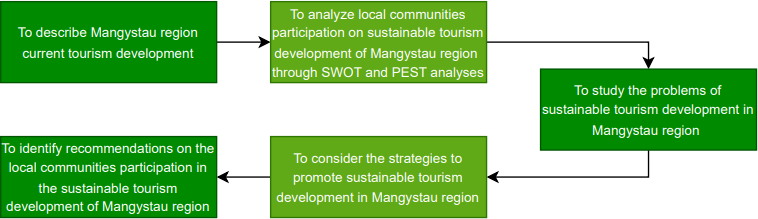
\includegraphics[width=0.8\textwidth]{assets/337}
	\caption*{}
\end{figure}

{\bfseries Fig. 1 - Research conceptual framework}

\emph{Study field.} Mangystau is located in the southwestern part of
Kazakhstan (Fig. 2), and a region renowned for its rich history,
cultural significance, and natural beauty. The landscape is marked by
vast deserts, unique rock formations, underground mosques, and the
Caspian Sea coastline. Historically, Mangystau served as a critical
crossroads for traders and travelers, leaving behind a rich array of
cultural and archaeological treasures. Despite these natural and
cultural assets, Mangystau remains relatively unknown as a tourist
destination in Kazakhstan, presenting both challenges and opportunities
for sustainable tourism development {[}4,5,13{]}.

\begin{figure}[H]
	\centering
	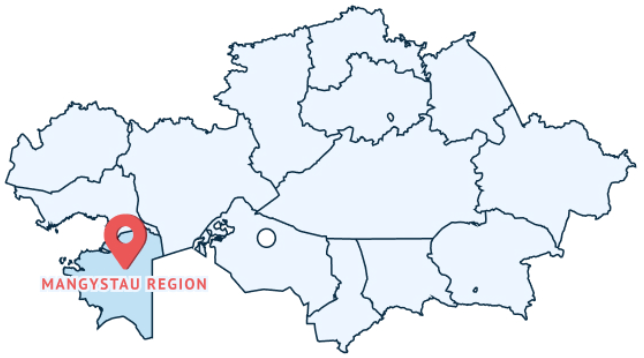
\includegraphics[width=0.8\textwidth]{assets/338}
	\caption*{}
\end{figure}

{\bfseries Fig. 2 -- The location of Mangystau region {[}13{]}}

The region is home to a diverse population with communities that have
maintained their traditions, languages, and customs for generations.
These communities play a pivotal role in Mangystau's sustainable tourism
strategy, as their participation can significantly enhance the
authenticity and sustainability of tourism initiatives. To maximize this
potential, it is essential to assess the strengths, weaknesses,
opportunities, and threats associated with local community involvement
in tourism.

Table 1 outlines the protected natural areas in the Mangystau region,
highlighting their size, location, and the government bodies responsible
for their management.

{\bfseries Table 1 -- Mangystau region's specially protected natural areas
{[}14{]}}

\begin{longtable}[]{@{}
  >{\raggedright\arraybackslash}p{(\columnwidth - 8\tabcolsep) * \real{0.0795}}
  >{\raggedright\arraybackslash}p{(\columnwidth - 8\tabcolsep) * \real{0.2502}}
  >{\raggedright\arraybackslash}p{(\columnwidth - 8\tabcolsep) * \real{0.1446}}
  >{\raggedright\arraybackslash}p{(\columnwidth - 8\tabcolsep) * \real{0.1539}}
  >{\raggedright\arraybackslash}p{(\columnwidth - 8\tabcolsep) * \real{0.3719}}@{}}
\toprule\noalign{}
\begin{minipage}[b]{\linewidth}\raggedright
№
\end{minipage} & \begin{minipage}[b]{\linewidth}\raggedright
The name of specially protected natural areas
\end{minipage} & \begin{minipage}[b]{\linewidth}\raggedright
Area, hectare
\end{minipage} & \begin{minipage}[b]{\linewidth}\raggedright
Location
\end{minipage} & \begin{minipage}[b]{\linewidth}\raggedright
Authority
\end{minipage} \\
\midrule\noalign{}
\endhead
\bottomrule\noalign{}
\endlastfoot
1 & Ustyurt State Nature Reserve & 223342 & Karakiyansky district &
Forestry and Wildlife Committee Ministry of Ecology, Geology and Natural
Resources of the Republic of Kazakhstan \\
2 & Aktau-Buzachinsky State Nature Reserve (zoological) & 170000 &
Tupkaragan district & Forestry and Wildlife Committee Ministry of
Ecology, Geology and Natural Resources of the Republic of Kazakhstan \\
3 & Karakiya-Karakol State Nature Reserve (zoological) & 137500 &
Karakiyansky district & Forestry and Wildlife Committee Ministry of
Ecology, Geology and Natural Resources of the Republic of Kazakhstan \\
4 & Kenderli-Kayasan State Protected Area & 1230290 & Karakiyansky
district & Forestry and Wildlife Committee Ministry of Ecology, Geology
and Natural Resources of the Republic of Kazakhstan \\
5 & Mangyshlak Experimental Botanical Garden & 39 & Aktau city & Science
Committee of the Ministry of Science and Higher Education of the
Republic of Kazakhstan \\
\end{longtable}

{\bfseries Results and discussion.} By utilizing the SWOT framework, the
research will systematically evaluate the internal and external factors
affecting sustainable tourism in the Mangystau region. Additionally,
existing data from government reports, academic journals, and industry
publications will be analyzed to support the primary data findings.

Fig. 3 offers a SWOT analysis of tourism development, emphasizing
strengths such as government backing and cultural richness, while also
noting weaknesses like limited training and infrastructure. It outlines
opportunities in sustainable tourism and community-driven initiatives,
and recognizes threats including environmental damage and cultural loss.
This analysis provides a strategic perspective on factors affecting
tourism development {[}15{]}.

\begin{figure}[H]
	\centering
	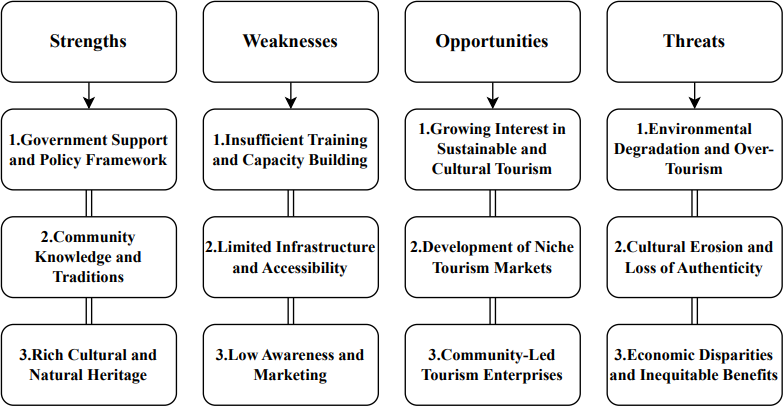
\includegraphics[width=0.8\textwidth]{assets/339}
	\caption*{}
\end{figure}

{\bfseries Fig. 3 -- SWOT analysis result {[}2{]}}

\emph{Strengths.} The Kazakh government prioritizes tourism for economic
diversification and has implemented policies to promote sustainable
tourism, including investments in infrastructure and eco-friendly
practices. Mangystau is rich in cultural landmarks, including the
Beket-Ata Underground Mosque, Shakpak-Ata Necropolis, and ancient
petroglyphs. These sites provide a deep insight into the
region\textquotesingle s history and identity, forming a strong
foundation for cultural tourism. The region\textquotesingle s natural
landscapes, such as deserts, cliffs, and the Caspian Sea coastline, are
home to rare species, making it an ideal spot for eco-tourism. Landmarks
like the Karagiye Depression and Ustyurt Plateau attract adventure
tourists and nature enthusiasts. Local communities maintain a rich
cultural heritage through traditional crafts, music, dance, and oral
histories, which can be integrated into tourism to offer visitors an
authentic experience and support local economies. Indigenous knowledge
of the region's natural and cultural resources is crucial for
sustainable tourism. Local guides can share insights into historical
sites, traditional uses of plants, and the spiritual significance of
natural landmarks. Mangystau region has specially protected natural
areas (Table 2), which can be popular places for the tourists.

\emph{Weaknesses.} The region\textquotesingle s vast distances between
attractions, underdeveloped road networks, and lack of public
transportation make it challenging for tourists to explore. The scarcity
of diverse accommodations and essential services like restaurants and
visitor centers further limits tourism growth. Mangystau is not widely
recognized as a tourist destination, and local communities often lack
the resources and expertise for effective marketing. This hinders the
region's ability to attract tourists and generate revenue. Many locals
have limited experience in tourism, particularly in hospitality and
foreign languages. Although some training programs exist, ongoing
education is needed to meet industry standards and support sustainable
tourism development.

\emph{Opportunities.} With increasing global interest in sustainable and
cultural tourism, Mangystau's rich heritage and diverse ecosystems
position it well to attract tourists seeking authentic and eco-friendly
experiences. The region\textquotesingle s rugged landscapes are ideal
for adventure tourism, while its religious sites can draw pilgrims.
There is also potential for health and wellness tourism, leveraging
natural hot springs and tranquil environments. Empowering local
communities through tourism enterprises ensures that the economic
benefits are shared equitably. Social enterprises and cooperatives can
create jobs for marginalized groups and reinvest profits into community
development.

\emph{Threats.} Without careful management, tourism growth could lead to
environmental degradation, over-tourism, and strain on infrastructure.
Waste and pollution are particular concerns, especially in remote areas
with limited infrastructure. The commercialization of cultural practices
for tourism can lead to a loss of authenticity and cultural erosion. It
is essential to preserve the region's cultural identity while promoting
tourism. Over-reliance on tourism as a primary economic driver can make
local communities vulnerable to external shocks, such as economic
downturns or natural disasters. Diversifying the economy and developing
resilience strategies are necessary for long-term stability.

\emph{Problems in Developing Sustainable Tourism.} The environment of
Mangystau is defined by fragile desert ecosystems that are highly
vulnerable to damage. The region\textquotesingle s arid climate and
limited water resources make it especially susceptible to the impacts of
tourism. Unregulated tourism activities can result in pollution, habitat
destruction, and the depletion of these scarce natural resources.
Achieving a balance between tourism development and the preservation of
these sensitive ecosystems is a major challenge {[}16{]}.

Mangystau currently lacks the infrastructure needed to support a
significant increase in tourist numbers. The region\textquotesingle s
roads, public transportation, accommodations, and waste management
systems are underdeveloped, making it challenging to meet the needs of
both tourists and local residents. Developing this infrastructure in a
sustainable way requires substantial investment and careful planning to
ensure it meets regional needs without exacerbating environmental issues
{[}17-18{]}.

Developing sustainable tourism requires a solid understanding of
environmental conservation and community involvement. In Mangystau,
there is a lack of local expertise in sustainable tourism practices,
which can hinder the effective implementation of such initiatives.
Additionally, without proper education and training, local communities
may not fully benefit from tourism or might unintentionally contribute
to environmental degradation.

While sustainable tourism seeks to balance economic development with
environmental and cultural preservation, this balance can be difficult
to achieve. The initial costs of creating sustainable infrastructure and
training programs can be high and the financial returns may not be
immediate. Moreover, ensuring that tourism generates sufficient income
to support local communities without overexploiting resources requires
careful management.

Mangystau is home to a rich cultural heritage with deep-rooted
traditions and customs. If not managed carefully, the influx of tourists
can lead to the erosion of these cultural values and practices. There is
a risk that tourism could commercialize or exploit cultural elements,
resulting in a loss of authenticity. It is crucial to ensure that
tourism development respects and preserves local culture for sustainable
growth {[}16,18{]}.

\emph{Strategic Framework for Sustainable Tourism Development.}
Sustainable tourism in Mangystau is a powerful tool for environmental
protection, economic development, and cultural preservation, with local
communities playing a central and indispensable role in its success. The
enhancement of infrastructure, such as roads and eco-lodges, not only
makes the region more accessible and comfortable for tourists but
directly benefits local communities, who are crucial to the development
process. By actively participating in promoting cultural heritage
through festivals and the preservation of historic sites, local
residents are empowered to take pride in their traditions, sharing them
with visitors while safeguarding these cultural elements from
disappearing (Table 2).

{\bfseries Table 2 -- Strategic Framework for Sustainable Tourism
Development in Mangystau}

\begin{longtable}[]{@{}
  >{\raggedright\arraybackslash}p{(\columnwidth - 6\tabcolsep) * \real{0.1905}}
  >{\raggedright\arraybackslash}p{(\columnwidth - 6\tabcolsep) * \real{0.3174}}
  >{\raggedright\arraybackslash}p{(\columnwidth - 6\tabcolsep) * \real{0.2539}}
  >{\raggedright\arraybackslash}p{(\columnwidth - 6\tabcolsep) * \real{0.2382}}@{}}
\toprule\noalign{}
\begin{minipage}[b]{\linewidth}\raggedright
Strategic Objective
\end{minipage} & \begin{minipage}[b]{\linewidth}\raggedright
Action Steps
\end{minipage} & \begin{minipage}[b]{\linewidth}\raggedright
Expected Outcome
\end{minipage} & \begin{minipage}[b]{\linewidth}\raggedright
Key Stakeholders
\end{minipage} \\
\midrule\noalign{}
\endhead
\bottomrule\noalign{}
\endlastfoot
Enhance Infrastructure & Upgrade roads, develop eco-lodges, improve
public transportation & Increased accessibility and comfort for tourists
& Government, private sector, local communities \\
Promote Cultural Heritage & Create and promote cultural festivals,
invest in preserving historic sites & Increased tourist interest in
cultural sites, preservation of traditions & Government, local
communities, NGOs \\
Develop Niche Markets & Identify and promote adventure tourism, health
and wellness tourism, and religious tourism & Diversification of tourism
offerings, attraction of niche markets & Tourism operators, local
entrepreneurs, international marketing partners \\
Foster Community-Led Enterprises & Provide training and financial
support for community-run guesthouses, craft cooperatives, and guided
tours & Increased community empowerment, equitable distribution of
tourism benefits & Local communities, NGOs, microfinance institutions \\
Ensure Environmental Sustainability & Implement strict waste management
protocols, limit visitor numbers in sensitive areas, promote
eco-friendly tourism activities & Preservation of natural resources,
reduction of tourism-related degradation & Environmental agencies, local
communities, eco-tourism organizations \\
Marketing and Global Awareness & Develop a comprehensive digital
marketing strategy, engage with international travel bloggers, and
partner with global eco-tourism organizations & Improved global and
domestic recognition of Mangystau as a tourist destination & Government,
digital marketing firms, international tourism bodies \\
\end{longtable}

The development of niche markets, including adventure, wellness, and
religious tourism, provides local entrepreneurs with unique
opportunities to create and offer experiences that are deeply rooted in
the region\textquotesingle s distinct characteristics. Community-led
enterprises, such as guesthouses, craft cooperatives, and guided tours,
ensure that the economic benefits of tourism are distributed equitably
among residents, enhancing community empowerment and fostering a strong
sense of ownership over Mangystau's natural and cultural resources.

Environmental sustainability is another critical pillar, with local
communities playing a vital role in implementing eco-friendly practices
like strict waste management and controlling visitor numbers in
sensitive areas. This collaboration helps preserve
Mangystau\textquotesingle s unique landscapes and biodiversity,
attracting environmentally conscious tourists and contributing to
long-term economic stability that benefits the community.

A comprehensive digital marketing strategy, involving local communities
and connecting with international travel bloggers and global eco-tourism
organizations, can significantly boost Mangystau's recognition as a
premier tourist destination. This not only stimulates the local economy
but also ensures that tourism development aligns with the values and
needs of the residents. By involving local communities in every aspect
of tourism planning and development, sustainable tourism in Mangystau
guarantees that economic growth, cultural preservation, and
environmental protection are achieved in a way that prioritizes the
well-being of current residents and secures a thriving future for
generations to come. This community-centered approach helps prevent the
adverse effects of over-tourism, such as environmental degradation and
cultural erosion, and supports the creation of a resilient tourism
industry that meets the long-term needs of the region and its people.

{\bfseries Conclusion.} The Mangystau region of Kazakhstan offers a unique
opportunity for sustainable tourism development, where the active
participation of local communities is both vital and necessary. The SWOT
analysis reveals that while the region has considerable strengths in its
cultural and natural heritage, it also faces significant challenges
related to infrastructure, marketing, and capacity building.

Sustainable tourism involves the planning and management of tourism
activities in a way that ensures the long-term preservation of the
environment, promotes social equity, and supports economic
sustainability. It focuses on reducing negative impacts on the
environment and local communities while maximizing benefits for all
involved. In Mangystau, sustainable tourism would mean protecting the
region\textquotesingle s natural and cultural assets while promoting
economic development and enhancing the well-being of local residents.

The tourism industry in Mangystau is still in its early stages. The
region is home to attractions like the Ustyurt Plateau, the coastline of
the Caspian Sea, the Karagiye Depression, and various historical sites
such as the underground mosques of Beket-Ata and Shakpak-Ata. Despite
these attractions, the region has yet to emerge as a prominent tourist
destination, primarily due to inadequate infrastructure, accessibility
challenges, and limited promotional efforts.

The sustainable development of tourism in Mangystau hinges on active
local participation, as the region faces numerous environmental,
cultural, and economic challenges. The delicate desert ecosystems are
particularly vulnerable to the adverse effects of uncontrolled tourism,
which can lead to pollution, habitat destruction, and resource
depletion. Addressing these issues requires thoughtful investment in
sustainable infrastructure, such as eco-friendly accommodations and
efficient waste management systems.

\begin{itemize}
\item
  Cultural preservation is also paramount, given
  Mangystau\textquotesingle s rich heritage. By involving local
  communities in tourism planning, the region can ensure that
  development respects and promotes its cultural traditions.
  Community-based tourism can empower residents by providing alternative
  sources of income and fostering cultural exchange.
\item
  Eco-tourism and cultural tourism present significant opportunities for
  Mangystau, attracting visitors who value environmental conservation
  and cultural appreciation. The Kazakhstan government, in collaboration
  with the private sector, can support these initiatives by enacting
  policies that promote sustainability and by providing incentives for
  eco-friendly businesses.
\item
  Public-private cooperation is crucial for financing infrastructure
  projects and ensuring equitable distribution of tourism benefits.
  Additionally, raising awareness about sustainable tourism practices
  among tourists, local communities, and businesses is essential for
  fostering a culture of sustainability.
\item
  Finally, ongoing research and monitoring are necessary to track the
  impact of tourism on the environment and local communities, enabling
  data-driven decision-making to address emerging challenges.
\end{itemize}

Local participation is key to ensuring that tourism development in
Mangystau is not only economically beneficial but also environmentally
and culturally sustainable.

To achieve sustainable tourism development, it is crucial to address
these weaknesses and threats through strategic planning, capacity
building, and active community involvement. Empowering local communities
to take ownership of tourism initiatives, providing them with the
necessary skills and resources, and ensuring that tourism development
aligns with their cultural values and environmental concerns are vital
steps toward a sustainable and inclusive tourism future for Mangystau.

By leveraging the region's strengths and capitalizing on new
opportunities, Mangystau can establish itself as a leading destination
for sustainable and cultural tourism in Central Asia. However, this will
require a collaborative effort between local communities, government
agencies, and international partners to create a tourism model that not
only attracts visitors but also preserves the region's cultural and
natural heritage for future generations. The success of sustainable
tourism in Mangystau ultimately hinges on the ability of all
stakeholders to work together toward shared goals, ensuring that tourism
benefits are equitably distributed and that the region\textquotesingle s
unique cultural and environmental assets are protected and celebrated.

The development of sustainable tourism in the Mangystau region presents
significant challenges as well as promising opportunities. Although the
region faces environmental, infrastructural, and cultural obstacles, the
potential benefits of sustainable tourism---including environmental
protection, economic growth, cultural preservation, community
empowerment, and long-term sustainability---are substantial. By
addressing these challenges and leveraging the advantages, Mangystau can
create a tourism industry that not only attracts visitors but also
preserves the region\textquotesingle s heritage.

Developing sustainable tourism in the Mangystau region presents a
promising opportunity for economic growth, environmental protection, and
cultural preservation. By adopting a comprehensive approach, that
balances the needs of tourists, local communities, and the environment,
Mangystau has the potential to become a leading example of sustainable
tourism in Kazakhstan and beyond. With the right strategies and
investments, the region can attract international visitors while
safeguarding its unique heritage for future generations.

\emph{{\bfseries Financing.} This research was funded by the Science
Committee of the Ministry of Science and Higher Education of the
Republic of Kazakhstan (Grant No. BR21882122 ``Sustainable Development
of Natural-Industrial and Socio-Economic Systems of the West Kazakhstan
Region in the Context of Green Growth: A Comprehensive Analysis,
Concept, Forecast Estimates and Scenarios'').}

{\bfseries References}

\begin{enumerate}
\def\labelenumi{\arabic{enumi}.}
\item
  Huang T., Wei J. Management strategies for museum night opening in
  China: a SWOT-TOWS analysis of Shanghai museums // Cogent Social
  Sciences. -2024. -Vol. 10(1). DOI:10.1080/23311886.2024.2327857
\item
  Cankül D., Cankül I., Aktepe B. Meal sharing economy: evaluation with
  SWOT analysis from host and local food tourists perspectives //
  Journal of Foodservice Business Research. -2024. -P. 1--22. DOI:
  10.1080/15378020.2024.2387388
\item
  Uchiyama Y., Kohsaka R. Strategies of Destination Management
  Organizations in Urban and Rural Areas: Using Text Analysis Method for
  SWOT Descriptions at Meta-level // International Journal of
  Hospitality \& Tourism Administration. -2021. -Vol. 24(1). -P.
  123-141. DOI:10.1080/15256480.2021.1953422
\item
  Ämırbaeva A.A., Ryskulov S.K., Ahmetova K.A. Qazaqstannyñ Mañğystau
  oblysynyñ auyldyq turizmınıñ äleuettı resurstary.~Agrarlyq naryq
  problemalary. -2023. --Vol. 2.
  -P.71-80.~https://doi.org/10.46666/2023-2.2708-9991.07 {[}in Kazakh{]}
\item
  Sabirova R.K., Andabaeva G.K., Mahanova A.N. Mañğystau öñirinde turizm
  türlerin damytu jäne onyñ auyldyq aumaqtardy damytuğa äseri.~Central
  Asian Economic Review. -2022(5), -P.142-154.
  https://doi.org/10.52821/2789-4401-2022-5-142-154 {[}in Kazakh{]}
\item
  Morea, J. P. Environmental justice, well-being and sustainable tourism
  in protected area management. Journal of Ecotourism. -2021. -Vol.
  20(3). -P. 250-269. DOI:10.1080/14724049.2021.1876072
\item
  Prayitno G. et al. Social capital for sustainable tourism development
  in Indonesia // Cogent Social Sciences. -2023. -Vol. 10(1).
  DOI:10.1080/23311886.2023.2293310
\item
  Nyiwul L. et al. Adoption of tools for sustainable tourism
  development: role of environmental vulnerability // Journal of Policy
  Research in Tourism Leisure and Events. -2024. -P. 1--23.
  https://doi.org/10.1080/19407963.2024.2317908
\item
  Hossain M.I., Kumar J., Islam Md.T. Antecedents of Sustainable Tourism
  Development in Sundarbans, Bangladesh with the Moderation of Political
  Instability and Mediation of Destination Resilience // Tourism
  Planning \& Development. -2024. -P. 1--29.
  DOI:10.1080/21568316.2024.2347222
\item
  Gani, A., Khairil, A., Mohamad, A., Samdin, Z. Attributes of
  successful public participation in planning for sustainable tourism in
  protected areas: A modified delphi study. -2015. --Vol. 23. --P.
  49-64.
\item
  Altaibayeva, Z., Pfeifer N., Shelomentseva V. \& Khamzina Sh.
  Assessment of the attractiveness and problems of the Territorial
  Natural Recreational Systems of North-East Kazakhstan by the
  population // Bulletin of the Karaganda University. Economy series.
  -2021. -Vol. 4(104), -P. 4-12. DOI:
  https://doi.org/10.31489/2021ec4/4-12
\item
  Pazylkhaiyr B., Assipova Zh.M., Bertocchi D. Development of tourism
  environmental management in Kazakhstan based on successful
  international experience // Bulletin of the Karaganda university
  economy series. -2023. -Vol. -110(2). -P. 79--89. DOI
  10.31489/2023Ec2/79-89
\item
  Welcome.kz. Unknown Mangystau Off-Road Tour -2024. {[}Online{]}.
  Available:
  https://welcome.kz/en/adventure/off-road-tours/unknown-mangystau-off-road
  {[}Accessed: Aug. 24, 2024{]}.
\item
  Adilet. Ob utverjdenii perechnya osobo ohranyaemih prirodnih
  territorii respublikanskogo znacheniya. -2017. {[}Online{]}.
  Available: https://adilet.zan.kz/rus/docs/P1700000593 {[}Accessed:
  Aug. 24, 2024{]}.
\item
  Font-Barnet A., Andreu M.N.-L. Research on tourism, well-being, and
  nature: a bibliometric analysis // Anatolia an International Journal
  of Tourism and Hospitality/Anatolia an International Journal of
  Tourism and Hospitality Research. -2021. -Vol. 34, -№ 2. -P. 163--175.
  DOI:10.1080/13032917.2021.2002699
\item
  Harish P., Rao Y.V. Research on sustainable tourism and biodiversity:
  a bibliometric analysis // Anatolia. -2024. -P. 1--21.
\item
  Kusumawardhani Y. et al. Smart tourism practice in the scope of
  sustainable tourism in emerging markets: a systematic literature
  review // Cogent Social Sciences. -2024. -Vol. 10(1).
  DOI:10.1080/23311886.2024.2384193
\item
  Niewiadomski P., Mellon V. Transitioning towards sustainable tourism
  in the Outer Hebrides: an evolutionary investigation // Tourism
  Geographies. -2023. -Vol. 26(2). -P. 214--236. DOI
  10.1080/14616688.2023.2283730
\end{enumerate}

\emph{{\bfseries Information about the author}}

Pazylkhaiyr B.M. -- Senior teacher of Department of Recreation geography
and tourism, Research Fellow, Al-Farabi Kazakh National University,
Almaty, Kazakhstan, e-mail: bauyrzhan.pazylkhaiyr@gmail.com.

\emph{{\bfseries Сведения об авторах}}

Пазылхайыр Б.М. -- старший преподаватель кафедры рекреационной географии
и туризма, научный сотрудник, Казахский национальный университет им.
аль-Фараби, Алматы, Казахстан, e-mail: bauyrzhan.pazylkhaiyr@gmail.com.\newpage
{\bfseries МРНТИ 06.52.35}

{\bfseries INDUSTRIAL AND INNOVATIVE DEVELOPMENT: CHALLENGES AND PROSPECTS
FOR KAZAKHSTAN}

{\bfseries \textsuperscript{1}A.S. Baktymbet, \textsuperscript{2}S.S.
Baktymbet, \textsuperscript{3}M.M. Idrisov, \textsuperscript{4}A.
Serikkyzy\textsuperscript{🖂}}

\textsuperscript{1}Kazakh University of Technology and Business, Astana,
Kazakhstan,

\textsuperscript{2}Academy of Political Management, Astana, Kazakhstan,

\textsuperscript{3}Institute of Industrial Development, Almaty,
Kazakhstan,

\textsuperscript{4}ALMAU, Almaty, Kazakhstan

{\bfseries \textsuperscript{🖂}}Corresponding author:
a.serikkyzy@almau.edu.kz

This paper explores the dynamics of industrial and innovative
development with a focus on Kazakhstan. It begins by examining the
principles guiding industrial and innovative strategies in foreign
countries, setting a comparative backdrop. The analysis then shifts to
Kazakhstan, detailing the major challenges confronting its manufacturing
industry, including structural inefficiencies and market constraints.
Further, the paper delves into the complexities and risks within
Kazakhstan\textquotesingle s oil and gas sector, highlighting both the
obstacles and potential growth areas. Finally, it assesses the prospects
and threats facing the country's mining and metallurgical complex,
offering insights into future trends and strategic recommendations. This
comprehensive review provides a nuanced understanding of
Kazakhstan\textquotesingle s industrial landscape and offers a framework
for navigating its evolving economic environment.

{\bfseries Key words:} industrial development, innovative strategies,
manufacturing challenges, economy growth, risks, prospects.

{\bfseries РАЗВИТИЕ ПРОМЫШЛЕННОСТИ И ИННОВАЦИЙ: ВЫЗОВЫ И}

{\bfseries ПЕРСПЕКТИВЫ ДЛЯ КАЗАХСТАНА}

{\bfseries \textsuperscript{1}А.С. Бактымбет, \textsuperscript{2}С.С.
Бақтымбет, \textsuperscript{3}М.М. Идрисов, \textsuperscript{4}Серікқызы
А.\textsuperscript{🖂}}

\textsuperscript{1}Казахский университет технологии и бизнеса им.
К.Кулажанова, г. Астана, Казахстан,

\textsuperscript{2}Академия политического менеджмента, г. Астана,
Казахстан,

\textsuperscript{3}Институт развития промышленности, г.Алматы,
Казахстан,

\textsuperscript{4}Университет ALMAU, Алматы, Казахстан,

e-mail: a.serikkyzy@almau.edu.kz

В данной статье рассматриваются динамика промышленного и инновационного
развития с акцентом на Казахстан. Сначала анализируются принципы,
руководствующие промышленными и инновационными стратегиями в зарубежных
странах, что создает сравнительный контекст. Затем внимание
переключается на Казахстан, где подробно рассматриваются основные
проблемы, с которыми сталкивается его производственный сектор, включая
структурные неэффективности и рыночные ограничения. В дальнейшем статья
исследует сложные вопросы и риски в нефтегазовом секторе Казахстана,
подчеркивая как препятствия, так и потенциальные области для роста.
Наконец, оцениваются перспективы и угрозы, с которыми сталкивается
горнодобывающий и металлургический комплекс страны, предлагаются
рекомендации по стратегии и прогнозирование будущих тенденций. Этот
всесторонний обзор предоставляет глубокое понимание промышленного
ландшафта Казахстана и предлагает основу для навигации в его
развивающейся экономической среде.

{\bfseries Ключевые слова:} промышленное развитие, инновационные стратегии,
проблемы производства, экономический рост, риски, перспективы.

{\bfseries ӨНЕРКӘСІП ЖӘНЕ ИННОВАЦИЯНЫҢ ДАМУЫ: ҚАЗАҚСТАННЫҢ}

{\bfseries ҚАУІПТІЛЕРІ МЕН БОЛАШАҒЫ}

{\bfseries \textsuperscript{1}Ә.С. Бақтымбет, , \textsuperscript{2}С. С.
Бақтымбет., \textsuperscript{3}М. М. Ыдырысов.,
\textsuperscript{4}А.Серікқызы\textsuperscript{🖂}}

\textsuperscript{1}Қ.Құлажанов атындағы Қазақ технология және бизнес
университеті, Астана қ, Қазақстан,

\textsuperscript{2}Саяси менеджмент академиясы, Астана қ, Қазақстан,

\textsuperscript{3}Өнеркәсіптік даму институты, Алматы қ, Қазақстан,

\textsuperscript{4}Алматы менеджмент университеті, Алматы қ, Қазақстан,

e-mail: a.serikkyzy@almau.edu.kz

Бұл мақалада Қазақстанға баса назар аудара отырып, өнеркәсіптік және
инновациялық даму динамикасы қарастырылады. Алдымен шет елдердегі
өнеркәсіптік және инновациялық стратегияларды басқаратын принциптер
талданады, бұл салыстырмалы контекст жасайды. Содан кейін назар
Қазақстанға ауысады, онда құрылымдық тиімсіздіктер мен нарықтық
шектеулерді қоса алғанда, оның өндірістік секторының алдында тұрған
негізгі проблемалар егжей-тегжейлі қарастырылады. Одан әрі мақала
Қазақстанның мұнай-газ секторындағы күрделі мәселелер мен тәуекелдерді
зерттеп, кедергілерді де, өсу үшін әлеуетті салаларды да атап көрсетеді.
Ақырында, елдің тау-кен және металлургия кешенінің болашағы мен
қауіптері бағаланады, стратегия бойынша ұсыныстар және болашақ
тенденцияларды болжау ұсынылады. Бұл жан-жақты шолу Қазақстанның
өнеркәсіптік ландшафтын терең түсінуге мүмкіндік береді және оның дамып
келе жатқан экономикалық ортасында навигация үшін негіз ұсынады.

{\bfseries Түйін сөздер:} Өнеркәсіптік даму, инновациялық стратегиялар,
өндіріс проблемалары, экономикалық өсу, тәуекелдер,
перспективалар{\bfseries .}

{\bfseries Introduction}. The global landscape of industrial and innovative
development is continuously evolving, influenced by varying national
strategies and economic conditions. As nations adapt to shifting
technological advancements and market demands, understanding these
dynamics becomes crucial for assessing their own industrial policies and
growth trajectories. This paper provides an in-depth examination of
industrial and innovative development principles, contrasting them with
the unique challenges and opportunities faced by Kazakhstan.

Beginning with an overview of successful industrial strategies employed
by foreign states, the study sets the stage for a comparative analysis.
It then shifts focus to Kazakhstan, exploring the significant hurdles
encountered by its manufacturing sector, which include structural
inefficiencies and competitive pressures. The paper further investigates
the complex landscape of Kazakhstan's oil and gas industry, identifying
key risks and potential growth avenues. Additionally, it assesses the
prospects and existing threats within the mining and metallurgical
complex, offering a comprehensive view of the sector's evolving
landscape.

By integrating international perspectives with a detailed analysis of
Kazakhstan\textquotesingle s industrial environment, this paper aims to
provide valuable insights for policymakers, industry leaders, and
researchers interested in understanding and shaping Kazakhstan's
economic future.

{\bfseries Methods. Principles of industrial-innovative development in
foreign states.} If we look at international experience, we can identify
common principles and approaches for organizing and implementing state
policies in industrial-innovative development.

1. System of industrial-innovative development management.

Industrial countries generally have a similar organizational structure
for state management of industrial development. The main elements of
this structure are:

1) Clear legislative regulation of industrial policy, which allows for
centralized and balanced industrial policy throughout the country,
systematizes and focuses the process and conditions of state support for
industry.

2) A central government body responsible for industrial development
policy, related services, and their promotion in international markets
(its tasks include formulating industrial-innovative development policy
considering the state's strategic priorities, creating a comprehensive
system of incentives and support measures for industrial-innovative
projects and industrial clusters, conducting trade policy aimed at
creating opportunities for expanding existing and new productions).

3) A coordinated system of institutions supporting industrial-innovative
development, including industrial development funds or agencies.

4) Large state or national private companies, specifically designated by
the state, with powers to attract investments and implement large
industrial projects and establish production in new sectors.

5) A unified scientific, technological, and innovation policy, directed
by plans, strategies, and programs of sectoral ministries and agencies.

2. Focus on high-value-added exports rather than commodities.

The experience of countries (Ireland, Canada, Vietnam, Botswana, Saudi
Arabia, Morocco) that have successfully diversified their economies
shows that state support is often complemented by a comprehensive
export-oriented industrial policy, focused on high-value-added
manufacturing sectors and products, through investments in productivity,
human capital, transportation-logistics infrastructure, and technology
transfer.

In Ireland, the export growth of manufacturing products between 2010 and
2016 was 174 {[}1{]}. This was supported by a state policy focused on
business development. For instance, the country has established a
favorable tax regime and provides financial assistance for the creation
of companies and their entry into international markets.

Another example is Vietnam, where the government has introduced a new
economic development model since 2010, involving restructuring of
industry and services, with an emphasis on supporting the production of
high-tech goods {[}1{]}. This led to the formation of a favorable
investment regime, significantly increasing foreign direct investment
and creating 135 industrial and export zones {[}1{]}.

Canada has developed a state support system for exporters with key
elements including {[}2{]}:

- Consulting services for Canadian companies on research and target
market selection abroad (export preparation, market potential
assessment, network identification, and problem-solving).

- The MY TCS online platform -- access to market information and
business opportunities.

- The Can Export program -- financial support for a wide range of export
operations to increase the competitiveness of Canadian companies,
providing up to 50 million dollars over 5 years in direct financial
support for small and medium-sized exporters, funding companies from any
sector, covering 50\% of expenses.

- Financial support for business associations to create or expand
international cooperation.

- Business Women in International Trade -- providing targeted products
and services for women entrepreneurs aiming to enter global markets.

Canadian Technology Accelerators -- supporting high-growth Canadian
companies ready to enter global ICT and clean technology markets
{[}2{]}.

Thus, the key driver for export diversification is the private sector,
and states support their enterprises to develop and expand their export
capabilities through increased access to external markets beyond their
small domestic economies. In many countries, industrial growth is linked
to creating favorable conditions for access to large developed markets
(e.g., export subsidies, tax breaks, and easier financing).
High-value-added exports stimulate the production of quality goods,
work, and services, accelerates economic development, attracts foreign
capital into the manufacturing sector, and helps diversify revenue
sources in unstable global commodity markets.

3. International cooperation through integration into global value
chains.

Global value chains (GVCs) refer to the sequence of operations in which
products and services, undergoing various stages of development and
processing in different countries due to the global nature of the
economy, gain value (from the consumer's perspective).

Almost all countries aim to integrate into global value chains, which
enables technology transfer and enhances the country\textquotesingle s
industrial potential. However, developing countries must adhere to free
market rules -- offering the best quality at minimal cost {[}3{]}.

4. Development of value chains through attracting global players in
manufacturing sectors.

Transnational companies play a crucial role in global value chains. The
acceleration of globalization and the worldwide distribution of
available raw materials, cheap labor, and potential markets have led
transnational companies to benefit from maintaining geographically
separated production facilities, research and development centers, and
markets. The primary value is created not in the physical production of
goods but in high-tech areas with a concentration of highly qualified
labor.

Conversely, concentrating highly qualified specialists, scientific
infrastructure, and engineering systems in manufacturing industries
allows countries to increase competencies in advancing in the value
chain, moving from lower to middle and upper-tier production. The main
distinctions of these product categories are the complexity of the
produced goods and their dependence on primary raw materials.

Lower-tier products typically use primary raw materials directly, whose
prices are often set on commodity exchanges and are fluctuating, leading
to variability in production volume and export depending on external
conditions. On the other hand, middle and upper-tier products have more
stable production and are less dependent on primary raw material prices,
as high technology and scientific labor constitute a larger portion of
their cost.

Therefore, developing countries focus on creating attractive offers for
transnational companies, balanced by the "price/quality" criterion. Key
aspects of integrating into global value chains include developing a
strong scientific-technological base, building a qualified workforce,
effectively using opportunities within international integration
associations, developing trade agreements with promising partners, and
implementing cluster policies to enhance value chains and
competitiveness within the country.

In Kazakhstan, further integration into global value chains is
necessary, with an expansion of cooperation with existing and new
transnational companies. Developing relationships with transnational
companies already operating in Kazakhstan should be based on mutually
beneficial cooperation considering Kazakhstan\textquotesingle s
interests. This will be achieved through expanding the range of produced
goods and deepening production to diversify and complicate the
country\textquotesingle s economy.

It should be noted that several global transnational companies (e.g.,
Arcelor Mittal, POSCO, LOTTE, Schneider Electric) are currently
operating in the country {[}1{]}. However, these companies are either
working with Kazakh enterprises in lower-tier production, outdated
products, or have just begun fruitful cooperation. Therefore, a balanced
and planned approach to cooperation with transnational companies is
needed to develop and deepen existing cooperation. A notable example of
integration into global value chains in Kazakhstan is the limited
liability partnership "POSUK Titanium," which produces titanium slabs
that are subsequently supplied to Boeing through the value chain
{[}1{]}.

Attracting new transnational companies should also align with the
state\textquotesingle s interests in achieving set goals, specifically
producing new high-value-added goods and exporting to global markets
through the distribution channels of transnational partners.

5. Implementing tools for attracting global players to integrate into
global value chains.

One of the primary tasks for attracting foreign investors should be
focusing on global leaders in manufacturing industries that have their
distribution channels in the global value chain.

Investment planning and integration into global value chains will
include implementing a unified map of priority goods and services. This
tool involves identifying a list of the most promising goods/product
groups for localization within the country, considering workforce,
technological, and raw material availability, as well as export markets.

This list of goods addresses both state and business interests. From the
state's perspective, priority goods will focus on expanding product
range, diversification, and complexity of production. For businesses,
the list can serve as a guide for creating new productions with growth
potential and entry into external markets.

\begin{figure}[H]
	\centering
	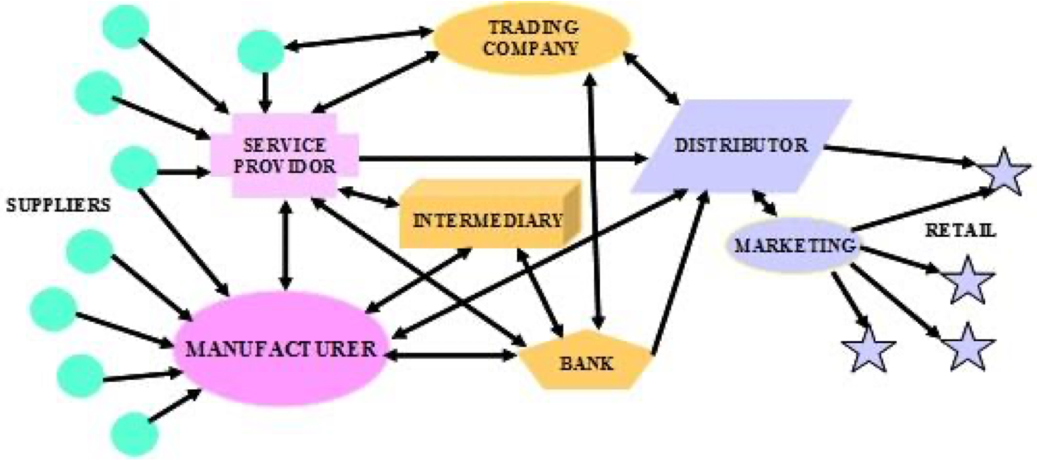
\includegraphics[width=0.8\textwidth]{assets/340}
	\caption*{}
\end{figure}

{\bfseries Figure 1 - Global value chains, commodity chains and production
networks {[}3{]}.}

6. Development of new production types for value addition in the market
and export.

The use of rare and rare-earth metals is crucial in complex industries
such as electronics, medicine, and computer manufacturing. The
development of finished products from these metals reflects the
technological advancement of the industry.

Currently, global demand for rare-earth elements is around 120,000 tons
per year {[}4{]}. However, the global market for rare-earth metals is
almost monopolized by Chinese production. Supply restrictions are
negatively impacting other countries\textquotesingle{} industries.
Consequently, major economies actively using rare-earth metals (USA,
Russia, Japan, Germany) are planning to reduce their dependency on
Chinese supplies. An example of this shift is the agreement between the
United States and Australia for joint mining and processing of minerals,
including rare-earth metals {[}5{]}.

Constant technological progress increases global demand for rare-earth
metal products. Moreover, upper-tier products, which involve high value
addition and technological complexity, are also significant.

Kazakhstan has substantial reserves and prospects for expanding its
mineral resource base of rare and rare-earth metals. The
republic\textquotesingle s production of these metals is carried out at
specialized enterprises.

Currently, the industry urgently needs investments, primarily for
improving infrastructure in mining regions. With effective use of rare
and rare-earth minerals, Kazakhstan can develop modern science and
technology sectors and market these metals globally.

{\bfseries Results}. {\bfseries Trends and challenges in Kazakhstan's
manufacturing industry.}

In 2022, the manufacturing sector\textquotesingle s output totaled 21.2
trillion tenge. The main contributors to the manufacturing industry are
metallurgy (44\% of the total sector), food production (19\%), machine
engineering (15\%), construction materials production (6\%), and
chemical industry (4\%) {[}6{]}.

Manufacturing accounts for 13.4\% of the country\textquotesingle s GDP.
In this regard, Kazakhstan remains a net importer for all categories of
goods except metallurgy. The highest net imports are observed in machine
engineering (7.6 trillion tenge), the chemical industry (1.4 trillion
tenge), and food production (0.9 trillion tenge) {[}6{]}.

The observed underutilization of production capacities indicates a low
level of competitiveness among domestic manufacturers: 70\% of
manufacturing enterprises have an average annual capacity utilization
rate of no more than 70\%, and the average annual capacity utilization
rate in the machine engineering sector has fluctuated between 25\% and
48\% in recent years. {[}6{]}.

{\bfseries Key challenges facing Kazakhstan's manufacturing industry.}

1. Low complexity of produced goods.

- Despite overall sector development, the share of raw materials in
exports remains at 66\%, while the proportion of local manufacturing
enterprises engaged in innovative activities is only 14.8\%.
Consequently, Kazakhstan has a negative economic complexity index
(-0.47) and ranks 88th out of 133 countries in this indicator, trailing
behind neighboring countries with similar economies (Russia - 53rd place
(0.19), Turkey - 40th place (0.61), and Belarus - 29th place (0.91))
{[}7{]}.

- In Kazakhstan, the depth of processing in raw material sectors is low,
with most products being exported as intermediate raw materials. For
example, 77\% of lead, 87\% of aluminum, and 99\% of copper are exported
in an unprocessed or minimally processed state {[}8{]}.

- Despite having a raw material base, Kazakhstan has not developed a
significant gas or petrochemical sector, and only in 2022 was the first
large-scale gas chemical project launched. Raw materials from Tengiz,
Kashagan, and Karachaganak contain high levels of fatty gas fractions
(ethane, propane, butane) necessary for gas chemical production.
Currently, fatty fractions are only extracted from raw materials from
the Tengiz field, which supplies polypropylene production (KPI) {[}8{]}.

Additionally, existing enterprises face raw material unavailability and
shortages: the volume of imported raw materials and components for the
manufacturing sector exceeds 50\%, which increases production costs and
creates barriers to establishing high-tech manufacturing. For instance,
imports constitute a significant portion of raw materials and components
for industrial equipment, vehicles, and agricultural machinery, while
the main output in machine engineering comprises simple assembly
operations with minimal localization.

- The insufficient level of international technology and standard
implementation in production is another factor reducing the economic
complexity index. This process requires technological upgrades and
substantial investments, which, in turn, affects the competitiveness of
domestic products.

2. Wear and low energy efficiency of production.

- The average level of wear is 41\%, with higher levels in the
production of metal products, beverages, weapons, military equipment,
and other machine engineering products exceeding 45\% {[}8{]}.

- Energy costs in Kazakhstan\textquotesingle s mining and metallurgical
complex are among the highest in the world. With energy intensity at 1.6
tons of oil equivalent per thousand USD, Kazakhstan\textquotesingle s
products lag significantly behind developing and developed markets,
where this figure ranges from 0.2 to 0.9 tons of oil equivalent per
thousand USD {[}8{]}.

{\bfseries Discussion}. {\bfseries Problems, risks, and opportunities in
Kazakhstan\textquotesingle s oil and gas sector.} Oil and gas production
continues to have a significant impact on Kazakhstan\textquotesingle s
economy: in 2022, the sector\textquotesingle s gross added value (GAV)
amounted to 11\% of GDP, with the sector\textquotesingle s share in
total goods exports exceeding 50\%, and in net investment inflow --
almost 40\% {[}8{]}.

Annually, oil production prospects in Kazakhstan fall short of
expectations. According to the current forecast, considering the
modernization of production at major fields, peak production is expected
to reach 104 million tons by 2030. Among the existing major fields, the
most significant decline in production is anticipated at Kashagan: in
2021, its expected peak production volume was reduced by 40\% compared
to the 2017 forecast {[}8{]}.

Additionally, one of the challenges is the depletion of deposits. For
instance, according to international experts\textquotesingle{}
forecasts, several major companies within KazMunayGas are expected to
see a 15-30\% decline in production by 2030. In this context,
sustainable reduction in production and the closure of depleting fields
are critical both from environmental and social perspectives. Moreover,
in the medium term, there is a risk of a shortage of oil raw materials
in addition to the expected gas deficit in 2024-2025, as local demand is
met by the KazMunayGas fields {[}8{]}.

International experts note that from 2017 to 2022, the forecast for
production at fields in the development and exploration stages also
dropped from 65 to 6 million tons {[}8{]}. The attractiveness of
exploring and developing new fields is limited by the pricing of raw
material supplies to the domestic market.

In addition to resource base constraints, the risk of raw material
shortages is exacerbated by the rapid growth in fuel consumption in
Kazakhstan. Per capita diesel fuel consumption (about 30\% of the demand
for petroleum products) significantly exceeds that of neighboring
countries. Moreover, fuel prices in Kazakhstan are among the lowest in
the region and the world, and the creation of common oil, gas, and
petroleum product markets within the EAEU in 2025 could lead to a flow
of lubricants to neighboring countries, further reducing domestic fuel
availability. According to the analytical company IHS Markit, if the
current consumption trajectory remains, by 2025, the demand for
petroleum products will reach 19 million tons of refined oil and exceed
the capacities of oil refineries {[}8{]}.

There are several opportunities for developing additional supply
corridors through the Trans-Caspian and Chinese routes. Current oil
transshipment through the Aktau port is 2.2 million tons per year with
the port\textquotesingle s technical capacity at 7 million tons per year
(available volume - 4.8 million tons). The Atasu - Alashankou pipeline
handles about 11 million tons per year, including 10 million tons of
transit. The technical capacity of this pipeline is approximately 17.5
million tons per year (available volume - 6.5 million tons) {[}8{]}.

In the gas transportation system, existing constraints mainly concern
transportation for domestic consumption. There is significant wear and
load on several key infrastructure facilities, such as the Beineu -
Bozoy - Shymkent pipeline and underground gas storage facilities.

{\bfseries Prospects and threats for Kazakhstan's mining and metallurgical
complex.}

Kazakhstan\textquotesingle s mining and metallurgical complex (MMC) is
one of the key drivers of the country\textquotesingle s economic growth:
in 2022, the total gross added value (GAV) from metal mining, coal,
lignite, and other solid minerals (SMs), as well as the metallurgical
industry, reached nearly 10\% of the economy, and over 25\% in exports.

However, the MMC faces key challenges and opportunities that will
determine its future development.

Kazakhstan is experiencing low levels of reserves prepared for
development, insufficient replenishment of reserves, a decline in
average ore content and increased complexity in processing ore bodies.
The availability of prepared copper reserves is 10-12 years; chromite
reserves suitable for open-pit mining have been depleted; the
availability of proven iron ore reserves suitable for open-pit mining is
20-25 years.

A critical factor affecting the situation is the low activity in
geological exploration. The legal reform in the mineral resource sector
has drastically changed its regulatory framework, providing more
competitive access to subsoil resources.

Currently, only 16\% of the country\textquotesingle s territory
available for exploration has been licensed. In 2022, the unit costs for
geological exploration in Kazakhstan were only \$63 per km², which is
significantly lower than the global average (\$88 per km² for metals)
and the figures for leading mining countries such as the USA, Canada,
and Australia (\$170 - \$300 per km²) {[}8{]}.

In addition to the insufficient replenishment of existing reserves, the
country has significant unrealized potential in the most rapidly growing
and promising metals used in modern batteries and electronics: nickel,
cobalt, and lithium. Another rapidly growing and unrealized category in
Kazakhstan is rare earth metals.

Another challenge for the sector is the rising cost of labor. Since
2000, the average cost per employee in the MMC has increased sevenfold,
reaching \$1,190 per month. However, wage increases have not been
accompanied by a comparable rise in labor productivity in the sector,
which remains at a relatively low level: in 2020, labor productivity in
Kazakhstan was \$62,000 per employee per year, compared to \$114,000 in
Peru and \$160,000 - \$200,000 in developed countries (Norway,
Australia, Canada, Ireland, Sweden) {[}8{]}.

Transportation and logistics constraints, such as the distance from key
markets, resulting in complex and costly logistics, as well as risks
related to the limited export transportation corridors, negatively
impact the competitiveness of Kazakhstan\textquotesingle s MMC products.

{\bfseries Conclusion.} In conclusion, the interplay between industrial and
innovative development strategies is pivotal in shaping the economic
future of nations. This paper has provided a comparative overview of
global industrial practices and analyzed the specific challenges and
opportunities faced by Kazakhstan. The examination of
Kazakhstan\textquotesingle s manufacturing sector reveals critical
inefficiencies and competitive constraints that require targeted reforms
and strategic investments. Similarly, the analysis of the oil and gas
sector highlights both significant risks and promising growth
opportunities that must be carefully managed to ensure sustainable
development.

The insights into Kazakhstan's mining and metallurgical complex
underscore the need for a balanced approach to harness its potential
while mitigating associated threats. By integrating international best
practices with a thorough understanding of local contexts, Kazakhstan
can better navigate its industrial and economic challenges.

Ultimately, the path forward for Kazakhstan involves leveraging its
existing strengths, addressing critical vulnerabilities, and adopting
innovative strategies to foster long-term growth and stability. This
comprehensive analysis serves as a foundational guide for policymakers,
industry stakeholders, and researchers dedicated to advancing
Kazakhstan's industrial capabilities and economic resilience.

\emph{{\bfseries Financing}. This work was financially supported by the
Science Committee of the Ministry of Science and Higher Education of the
Republic of Kazakhstan (grant AP1968020, 2023--2025).}

{\bfseries References}

\begin{enumerate}
\def\labelenumi{\arabic{enumi}.}
\item
  The Government of the Republic of Kazakhstan (2019). State Program for
  Industrial-Innovative Development of the Republic of Kazakhstan for
  2020-2025. URL: https://adilet.zan.kz/rus/docs/P1900001050 (date of
  application - 16.09.2024)
\item
  Grigorieva E. Supporting the Export of Agricultural Products in
  Canada. -2016. URL:
  https://cyberleninka.ru/article/n/sodeystvie-eksportu-produktsii-apk-v-kanade
  (date of application - 16.09.2024)
\item
  Todeva E., Rakhmatullin R. Industry Global Value Chains, Connectivity
  and Regional Smart Specialisation in Europe. -2016. --URL:
  http://www.bcned.co.uk/images/reports/research/JRC102801\_lfna28086enn.pdf
  (date of application - 16.09.2024)
\item
  Metal Mining The Rare Earth Metals: From Strength to Compactness.
  -2017. URL: https://metalmininginfo.kz/archives/4688 (date of
  application - 16.09.2024)
\item
  Prokhorov I. The Rare Earth Metals Market Shows Steady Growth. -2017.
  URL:
  https://www.gmprom.kz/analytics/rynok-redkozemelnyh-metallov-pokazyvaet-ustojchivyj-rost/
  (date of application - 16.09.2024)
\item
  Ministry of industry and construction of the Republic of Kazakhstan
  Growth in Kazakhstan\textquotesingle s manufacturing industry reached
  4.1\%. -2024. URL:
  https://www.gov.kz/memleket/entities/mps/press/news/details/727688?lang=en
  (date of application - 16.09.2024)
\item
  Karimov E. Economic Complexity Index: India and Kazakhstan. -2024.
  URL: https://economy.kz/?p=5210 (date of application - 16.09.2024)
\item
  The Government of the Republic of Kazakhstan The National Development
  Plan of the Republic of Kazakhstan until 2029. -2024. URL:
  https://adilet.zan.kz/rus/docs/U2400000611 (date of application -
  16.09.2024)
\end{enumerate}

\emph{{\bfseries Information about authors}}

Baktymbet A.S. - c.e.s., assistant professor at the Kazakh University of
Technology and Business, Astana, Kazakhstan, e-mail:
asembaktymbet@gmail.com;

Baktymbet S.S.-c.e.s, assistant professor, Academy of Political
Management, Astana, Kazakhstan, e-mail: saule\_sbs@mail.ru;

Idrisov M.M. - Director of the Institute of Industrial Development,
Almaty, Kazakhstan, e-mail: m.idrissov.kz@gmail.com;

Serikkyzy A .- PhD, associate professor ALMAU, Almaty, Kazakhstan,
e-mail: a.serikkyzy@almau.edu.kz

\emph{{\bfseries Сведения об авторах}}

Бактымбет Ә.С. - к.э.н., доцент Казахского университета технологий и
бизнеса, Астана, Казахстан

e-mail: asembaktymbet@gmail.com;

Бақтымбет С.С. -- к.э.н., доцент, Академия политического менеджмента,
Астана, Казахстан, e-mail: saule\_sbs@mail.ru;

Идрисов М. М. -- директор Института промышленного развития, Алматы,
Казахстан email: m.idrissov.kz@gmail.com;

Серіккызы А. - PhD, ассоциированный профессор ALMAU, Алматы, Казахстан,
e-mail: a.serikkyzy@almau.edu.kz\newpage
{\bfseries ҒТАМР 06.73.07}

{\bfseries Бағалы қағаздар нарығын мемлекеттік реттеу мәселелері}

{\bfseries Р.Қ. Елшібаев}

«Нархоз университеті» КЕАҚ, Алматы, Қазақстан

{\bfseries \textsuperscript{🖂}}Корреспондент-автор:
rakymzhan.yelshibayev@bk.ru

Елімізде қор биржасының белсенділігі айтарлықтай арта түсті. Әсіресе
жеке инвесторлар сегментінің кеңеюі байқалады. Ол елдегі экономикалық
тұрақтылыққа, инфляция деңейіне, халықтың нақты табысының өсуіне тікелей
байланысты. Сондықтан да елдегі тұрақтылық, халықтың әл-ауқатын арттыру,
экономикалық өсім, ақша-несие жүйесі, бизнес субъектілерінің
белсенділігі басты назарда болуы тиіс. Жеке тұлғалардың бағалы
қағаздарды сатып алуға қызығушылығының артуына пандемия да өзінің
ықпалын тигізді. Жеке инвесторлар банктік депозиттерге баламалы
көздерді, қосымша табыс табу жолдарын қарастыра бастады. Сонымен қатар
брокерлік қызметтерді цифрландыру барлық қызығушылық танытқандарға
инвестициялауға қол жетімділікті қамтамасыз етті.

2020жылдан бастап екінші деңгейлі банктерге брокерлік қызметті жүргізуге
рұқсат берілуі, олардың белсенділігін арттыра түсті. Қазір еліміздің
жекелеген банктері (Халық банк, Банк Центр Кредит) мобильді қосымшалары
арқылы бағалы қағаздарын сатуды іске асыра алады. Қазір тек ірі
компаниялар ғана емес шағын және орта бизнес субъектілерінің де бағалы
қағаздар нарығындағы белсенділігін жоғарылату бойынша жұмыстар жасалып
жатыр. Сондықтан да бағалы қағаздар нарығына бастапқы кезеңде
мемлекеттің араласуы, қолдау және реттеу бойынша жүйелі жұмыстар атқаруы
өте маңызды.

Мақалада елімізде қор нарығын дамытудың қажеттілігі және мемлекеттік
реттеу мәселелері қарастырылған. Бағалы қағаздар нарығын мемлекеттік
реттеудің маңызы, негізгі мақсаты және іске асыру құралдары мен негізгі
тәсілдері көрсетілген, сондай-ақ, өзекті мәселелері анықталып, оларды
шешу жолдары ұсынылған.

{\bfseries Түйін сөздер:} қор нарығы, бағалы қағаздар, эмитент, инвестор,
трейдер, брокер, диллер, мемлекеттік реттеу, Қазақстандық қор биржасы.

{\bfseries Вопросы государственного регулирования рынка ценных бумаг}

{\bfseries Р.К. Елшибаев}

НАО «Университет Нархоз», Алматы, Казахстан,

e-mail: rakymzhan.yelshibayev@bk.ru

В стране значительно возросла активность фондовой биржи. Особенно
заметно расширение сегмента частных инвесторов. Это напрямую зависит от
экономической стабильности в стране, уровня инфляции, роста реальных
доходов населения. Поэтому в центре внимания должны быть стабильность в
стране, повышение благосостояния населения, экономический рост,
денежно-кредитная система, активность субъектов бизнеса. На рост
интереса физических лиц к покупке ценных бумаг повлияла и пандемия.
Частные инвесторы начали рассматривать альтернативные источники
банковских депозитов, способы получения дополнительных доходов. Кроме
того, цифровизация брокерских услуг обеспечила всем желающим доступ к
инвестированию.

С 2020 года банки второго уровня получили разрешение на ведение
брокерской деятельности, что повысило их активность. Сейчас отдельные
банки страны (Народный банк, Банк Центр Кредит) могут осуществлять
продажу ценных бумаг через мобильные приложения. Сейчас ведется работа
по повышению активности на рынке ценных бумаг не только крупных
компаний, но и субъектов малого и среднего бизнеса. Поэтому очень важно,
чтобы государство на начальном этапе проводило системную работу по
вмешательству, поддержке и регулированию рынка ценных бумаг.

В статье рассматривается необходимость развития фондового рынка и
вопросы государственного регулирования в стране. Указаны важность,
основная цель, инструменты и методы осуществления государственного
регулирования рынка ценных бумаг, а также выявлены актуальные проблемы и
предложены пути их решения.

{\bfseries Ключевые слова:} фондовый рынок, ценные бумаги, эмитент,
инвестор, трейдер, брокер, дилер, государственное регулирование,
Казахстанская фондовая биржа.

{\bfseries ISSUES OF STATE REGULATION OF THE SECURITIES MARKET}

{\bfseries R.K. Yelshibayev}

JSC Narxoz University, Almaty, Kazakhstan,

e-mail: rakymzhan.yelshibayev@bk.ru

The activity of the stock exchange has increased significantly in the
country. The expansion of the segment of private investors is especially
noticeable. This directly depends on the economic stability in the
country, the level of inflation, and the growth of real incomes of the
population. Therefore, the focus should be on stability in the country,
improving the well-being of the population, economic growth, the
monetary system, and the activity of business entities. The pandemic
also influenced the growing interest of individuals in buying
securities. Private investors began to consider alternative sources of
bank deposits, ways to generate additional income. In addition, the
digitalization of brokerage services provided everyone with access to
investing.

Since 2020, second-tier banks have received permission to conduct
brokerage activities, which has increased their activity. Now individual
banks of the country (Halyk Bank, Bank Center Credit) can sell
securities through mobile applications. Now work is underway to increase
activity in the securities market not only of large companies, but also
of small and medium-sized businesses. Therefore, it is very important
that the state at the initial stage carries out systematic work to
intervene, support and regulate the securities market.

The article discusses the need to develop the stock market and issues of
government regulation in the country. The importance, main goal, tools
and methods of implementing state regulation of the securities market
are indicated, and current problems are identified and ways to solve
them are proposed.

{\bfseries Key words:} stock market, securities, issuer, investor, trader,
broker, dealer, state regulation, Kazakhstan Stock Exchange.

{\bfseries Кіріспе.} Елімізде бағалы қағаздар нарығын дамыту және реттеу
қаржы секторының тиімділігіне тікелей ықпал етеді. Сондықтан да бұл
мәселе мемлекет басшысының басты назарында. Қор биржасының жеткілікті
деңгейде дамымауы, халықтың қаржылық сауаттылығының төмендігі, бағалы
қағаздармен жұмыс жасауда қажетті білімдер мен дағдылардың болмауы
қарапайым халықтың алаяқтарға алдануына, қаржы пирамидасына сеніп
қалуына алып келеді. Осыған байланысты бұл бағытта
теориялық-әдістемелік, тәжірибелік, ғылыми ізденістердің қажеттілігі мен
маңыздылығы жоғары деп айтуға болады. Еліміз егемендігін алғаннан бастап
қазіргі кезге дейін бағалы қағаздар нарығына қатысты бірқатар
нормативтік-құқықтық актілер әзірленіп, жыл өткен сайын өзгерістер мен
толықтырулар енгізіліп отырды. Соның нәтижесінде бағалы қағаздарды
шығару мен айналымға енгізу бойынша экономикалық қатынастар жүйесінде
жаңа құқықтық орта қалыптастырылды. Алайда бағалы қағаздар нарығын
дамыту мен реттеудің жүйелі тәсілдерінің болмауынан бұл нарық бүгінгі
таңда өзінің инвестициялық функциясын жеткілікті деңгейде орындай алмай
отыр. Қазақстанның бағалы қағаздар нарығын дамыту мен мемлекеттік реттеу
аясындағы іргелі зерттеулердің тапшылығы мәселенің өзектілігін
көрсетеді.

{\bfseries Материалдар және әдістер.} Зерттеу жүргізу барысында
эмпирикалық, субъектілік-объектілік, жүйелік, дедуктивтік және
салыстырмалы талдау әдістері қолданылды. Бұл әдістердің әрқайсысы сәйкес
зерттеу міндеттерін шешу үшін функционалдық мүмкіндіктеріне байланысты
пайдаланылды. Бұл зерттеуде теориялық-эмпирикалық әдістерді қолдану
мемлекеттік реттеу объектісі ретінде Қазақстан Республикасы бағалы
қағаздар нарығының экономикалық мәнін неғұрлым тереңінен түсінуге
мүмкіндік берді.

Бағалы қағаздар нарығын мемлекеттік реттеу жүйесін инфрақұрылымдық
қамтамасыз етуді зерттеу кезінде ақпаратты жинау әдісі және қажетті
материалды тиімді іздеу, топтастыру, өңдеу және қорытындылау үшін
абстрактілеу әдісі ішінара қолданылды.

Нарықтың негізгі экономикалық көрсеткіштерін зерттей отырып автор
жүйелік және салыстырмалы талдау әдістерін қолданды.

Зерттеудің мақсаты -- бағалы қағаздар нарығын мемлекеттік реттеу жүйесін
жетілдіру және дамыту бағыттарын анықтау.

Зерттеу гипотезасы бағалы қағаздар нарығын реттеуді жетілдіру елімізде
қор нарығын дамыту мен тартымдылығын жоғарылатуға мүмкіндік
беретіндігімен сипатталады.

Мақаланың ғылыми жаңашылдығы бағалы қағаздар нарығын мемлекеттік реттеу
қазіргі кезге дейін қалай жүргізілді және алдағы уақытта қандай бағытта
даму қажеттілігін айқындау, нарықтағы өзекті мәселелер және оларды шешу
жолдарын ұсынуда көрініс тапқан.

Зерттеу нәтижелері. Мақаланың негізгі ғылыми нәтижесі бағалы қағаздар
нарығын мемлекеттік реттеудің өзекті мәселелері анықталып, оларды шешу
жолдары ұсынылды.

Бағалы қағаздар нарығы және оның жұмыс жасау механизмінің өзекті
мәселелерін зерттеумен көптеген ғалымдар және практик-мамандар айналысып
келеді. Зерттеу тақырыбы бойынша жарияланған еңбектердің көпшілігінде
елімізде қолайлы инвестициялық ахуалды қалыптастыру арқылы халықтың
әл-ауқатын жақсарту мәселелері қамтылған. Қор нарығын қарқынды дамытуда
және тиімді қызметін қамтамасыз етуде бағалы қағаздар нарығының рөлі,
мемлекеттің ықпал ету дәрежесі, қандай құралдар мен әдіс-тәсілдер арқылы
жоғары нәтижелерге қол жеткізуге болатындығы жеткілікті деңгейде
қарастырылмаған.

{\bfseries Нәтижелер мен талқылау.} Бағалы қағаздар нарығы осындай
қағаздардың эмиссиясы мен айналымы бойынша оның субъектілерінің
арасындағы экономикалық қатынастар жиынтығын білдіреді. Бағалы қағаздар
нарығының субъектілері ретінде эмитенттер, инвесторлар мен нарықтың
кәсіби қатысушыларын айта аламыз {[}1{]}.

Қазақстанда бағалы қағаздар нарығы екі үлкен бөлікке бөлінген:
ұйымдастырылған бағалы қағаздар нарығы және ұйымдастырылмаған бағалы
қағаздар нарығы.

Бағалы қағаздар нарығының қатысушыларын шартты түрде бірнеше топқа
бөлуге болады:

\begin{enumerate}
\def\labelenumi{\arabic{enumi}.}
\item
  Жеке және институционалдық инвесторлар.
\item
  Бағалы қағаздар шығаратын эмитенттер.
\item
  Бағалы қағаздар нарығының кәсіби қатысушылары (бағалы қағаздар
  нарығында қызметін жүзеге асыруға лицензиясы бар ұйымдар).
\item
  Сауданы ұйымдастырушылар (қор биржасы немесе орталық депозитарий)
  {[}2{]}.
\end{enumerate}

Бағалы қағаздар нарығын мемлекеттік реттеу - бұл бағалы қағаздар нарығы
қатысушыларының іс-әрекетін реттеуге бағытталған мемлекеттің
уәкілеттілік берген ұйымының іс-әрекеті.

Мемлекеттік реттеудің негізгі мақсаты -- бағалы қағаздар нарығының одан
әрі дамуы мен тиімді қызмет етуін қолдау. Ол келесілер арқылы қамтамасыз
етіледі:

\begin{itemize}
\item
  нарықтың барлық қатысушыларының жұмысына қолайлы жағдай жасау және
  реттеу;
\item
  нақты сұраныс және ұсыныс негізінде нарықтағы баға белгілеуге бақылау
  жүргізу;
\item
  нарықтағы ойыншылардың тәуекелінің сыйақысы үшін әлеуетті капиталды
  қайта бөлудің тиімді механизмін жасау;
\item
  контрагенттердің әртүрлі сипаттағы әділетсіз әрекеттерінен нарық
  қатсушыларын қорғау; Мәселен, әділетсіз бәсеке, инсайдерлік ақпаратпен
  сату, алаяқтық т.б. сақтау;
\item
  бағалы қағаздар сферасында тиімді салық салу жүйесін қалыптастыру;
\item
  жаңа нарықтарды ұйымдастыру, олардың құрылымдарын, бастамалары мен
  жаңашылдықтарын қолдау;
\item
  бағалы қағаздар нарығын дамыту кезінде қоғамдық мүдделердің бұзылуына
  жол бермеу {[}3{]}.
\end{itemize}

Бағалы қағаздар нарығын мемлекеттік реттеу тәсілдерін келесі сурет
түрінде көрсетуге болады (1-сурет).

Бағалы қағаздар нарығын мемлекеттік реттеу тәсілдері

{\bfseries 1 - сурет. Бағалы қағаздар нарығын мемлекеттік реттеу тәсілдері}

{\bfseries Ескерту -- зерттеулер негізінде автормен әзірленген}

«Бағалы қағаздар нарығы туралы» заңға сәйкес, мемлекеттік реттеу
органдары келесідей міндеттерді шешуі тиіс:

\begin{itemize}
\item
  бағалы қағаздар нарығының кәсіби қатысушыларының, эмитенттердің
  қызметіне қатысты міндетті талаптарды және оның стандарттарын
  белгілеу;
\item
  бағалы эмиссиялық қағаздар шығару мен эмиссиялар проспектісін тіркеу
  және ондағы қарастырылған шарттар мен міндеттемелерді эмитенттердің
  сақтауын бақылау;
\item
  бағалы қағаздар нарығының кәсіби қатысушыларының қызметін лицензиялау;
\item
  меншік иелерінің құқықтарын қорғау жүйесін құру және олардың
  құқықтарын қаржы нарығының кәсіби қатысушыларының және эмитенттердің
  сақтауын бақылау;
\item
  лицензиясыз кәсіпкерлік қызметпен айналысатын тұлғалардың іс-әрекетіне
  тиым салу және шектеу, сондай-ақ, бағалы қағаздар нарығы
  қатысушыларының кәсіби және білім деңгейін жоғарылатуды ұйымдастыру
  {[}4{]}.
\end{itemize}

Жоғарыда айтып өткеніміздей бағалы қағаздар нарығын реттеуді нарық
қатысушыларының өздері іске асыруы мүмкін. Ол үшін нарықтың кәсіби
қатысушылары (брокерлер мен дилерлер) коммерциялық емес ұйымдарға
бірігеді. Мұндай ұйымдардың мақсаты -- бағалы қағаздар нарығын реттеу
процесіне мемлекеттік реттеуші ұйымдармен бірге қатысу. Мұндай жағдайда
мемлекет өздерінің реттеуші функцияларының бір бөлігін береді. Алайда
мұндай ұйымдарды мемлекеттік деп атауға болмайды, оларды өзін-өзі
реттеуші ұйымдар деп атайды {[}5{]}.

Қазақстанда жалғыз толыққанды өзін-өзі реттейтін ұйым -- Қазақстандық
қор биржасы (KASE). Оның жарғысына сәйкес негізгі міндеттеріне мыналар
жатқызылады:

\begin{itemize}
\item
  бағалы қағаздар нарығында кәсіби қызметтің қолайлы шарттарын
  қамтамасыз ету;
\item
  нарықта кәсіби этика стандарттарын қолдау;
\item
  мемлекеттік реттеу органдарында кәсіби қатысушылардың мүдделерін
  қорғау;
\item
  бағалы қағаздармен операциялар жүргізудің ережелері мен стандарттарын
  белгілеу;
\item
  олардың орындалуын бақылау {[}6{]}.
\end{itemize}

KASE индексі қазақстандық бағалы қағаздар нарығының даму динамикасын
сипаттайтын негізгі индикатор болып табылады.

Қазір қазақстандық қор биржасында келесідей қаржы құралдары айналымда
жүр:

\begin{itemize}
\item
  жедел келісім-шарттар: стандартталған жеткізілмеген АҚШ долларындағы
  фьючерс;
\item
  ҚР қаржы министрлігімен берілген мемлекеттік бағалы қағаздар;
\item
  ҚР Ұлттық Банкімен берілген бағалы қағаздар;
\item
  ҚР Қаржы министрлігінің мемлекеттік мүлік және жекешелендіру
  департаментімен сатуға қойылған акциялардың мемлекеттік пакеті;
\item
  Екінші деңгейлі банктердің депозиттік сертификаттары;
\item
  Мемлекеттік емес бағалы қағаздар: облигациялар, жай, атаулы,
  артықшылығы бар акциялар.
\end{itemize}

Мемлекеттік бағалы қағаздардың табыстылығы жоғары емес, бірақ, олар
сенімділіктің жоғары дәрежесін иеленеді. Сондықтан да халықтың бір тобы
тәуекелге бармастан, өздерінің қаражаттарын осындай бағалы қағаздарға
салу дұрыс деп есептейді.

Қазақстандық қор биржасында мемлекеттік бағалы қағаздармен сауда жасау
тәсілі электрондық үздіксіз қарсы аукцион әдісі болып табылады. Ол
қойылған бағамға сәйкес ең жақсы қарсы баға бойынша жасырын контр
әріптеспен автоматты түрде мәміле жасауға негізделген. Сол себепті
абстрактілеу әдісі көзқарасы тұрғысынан мемлекеттік бағалы қағаздар
нарығының динамикасын бақылау едәуір күрделі және тиімсіз болып
көрінеді.

Автордың пікірі бойынша, нарықты реттеу мен дамыту жөнінде мемлекеттік
шаралардың тиімділігін бағалау үшін мемлекеттік емес бағалы қағаздардың
едәуір динамикалық нарығына және оның институционалдық инвесторына назар
аудару қажет. Сонымен қатар бағалы қағаздар нарығының дамуы елімізде
қаржы секторының дамуымен тікелей байланысты екендігін атап өту қажет.

Елімізде қаржы секторын дамытудың негізгі жеті бағыты анықталған. Олар
келесілер:

\begin{itemize}
\item
  қаржылық тұрақтылық және оған деген сенімді қолдау;
\item
  тұрақты дамуға көшу (инновациялар, технологиялар, бизнес-модельдер мен
  құзіреттіліктер);
\item
  қаржылық қызметті тұтынушылардың құқықтары мен мүдделерін қорғау;
\item
  экономиканы қаржыландыру және банктік сектордың дамуы;
\item
  қаржылық мүдделерді қорғау құралы ретінде сақтандыру нарығының дамуы;
\item
  экономиканы қаржыландырудың қосымша каналы ретінде бағалы қағаздар
  нарығын дамыту;
\item
  банктік емес сектор мен микроқаржыландыруды дамыту {[}7{]}.
\end{itemize}

{\bfseries Қорытынды.} Жүргізілген зерттеулер негізінде бағалы қағаздар
нарығын дамыту мен мемлекеттік реттеу жүйесіндегі мынадай өзекті
мәселелер анықталды:

\begin{itemize}
\item
  нарықтың шектеулі өтімділігі;
\item
  нарық субъектілерінің қызметін реттейтін заңдар мен басқа да
  нормативтік құжаттардағы кемшіліктер;
\item
  сапалы қаржылық құралдардың тапшылығы;
\item
  акционерлер өз кәсіпорнын қор нарығына шығарған жағдайда оны жоғалтып
  алудан қорқуы және жариялы IPO дан бас тартуы;
\item
  листингтік компаниялардың ашықтығының жеткілікті деңгейде болмауы;
\item
  инвесторлардың, әсіресе портфельдік және шағын кәсіби емес
  инвесторлардың құқытары мен мүдделерін қорғаудың нақты механизмінің
  болмауы.
\end{itemize}

Отандық бағалы қағаздар нарығын қажетті деңгейде дамыту үшін мемлекеттің
уәкілетті органы келесідей іс-шараларды жүзеге асыруы керек:

\begin{enumerate}
\def\labelenumi{\arabic{enumi}.}
\item
  Отандық қор нарығында айналымда болатын өтімді және сенімді қаржылық
  құралдардың тізімін кеңейту.
\item
  Тәуекелдерді басқару жүйесінің сапасын жоғарылата отырып, заманауи
  IT-технологиялардың көмегімен кәсіби қатысушылардың жұмыс жасау
  әдістерін жетілдіру арқылы қаржылық қызмет көрсету сапасын арттыру.
\item
  Эмитенттер мен олардың лауазымды тұлғаларының облигацияларды шығару
  мен орналастыру талаптарын бұзғаны үшін жауапкершілікті жоғарылату.
\item
  Облигацияларды ұстаушылардың өкілдерінің рөлін көтеру және
  функцияларын кеңейту;
\item
  Қазақстандық қор биржасына эмитенттер мен биржа мүшелеріне мониторинг
  жасау мақсатында қосымша функциялар беру.
\end{enumerate}

Зерттеу тақырыбы бойынша жүргізілген ізденістер, ғылыми және іскерлік
әдебиеттерді талдау мен қорытындылау нәтижесінде келесідей маңызды
міндеттерді шешуге назар аудару қажеттілігі анықталды:

\begin{itemize}
\item
  Бағалы қағаздар нарығының тұрақтылығын арттыру. Яғни, бағалы қағаздар
  нарығындағы тәуекелдердің алдын алу және төмендету бойынша іс-шаралар
  әзірлеу. Бағалы қағаздар нарығындағы инвесторлардың мүдделері мен
  құқықтарын қорғауды қамтамасыз ету.
\item
  Экономикалық интеграция жағдайында бағалы қағаздар нарығының
  тиімділігін жоғарылату. Бағалы қағаздар нарығында сұранысты
  ынталандыру мен көтеру, білікті инвесторлар институтының қызмет ету
  механизмін жетілдіру, брокерлік ұйымдардың функционалы мен
  мүмкіндіктерін кеңейту.
\item
  Инфрақұрылымды жетілдіру және бағалы қағаздар нарығын сапалы дамыту
  үшін оңтайлы жағдай жасау. Эмитенттерге қойылатын листигтік талаптар
  мен қор биржасының ресми тізімінің құрылымын реформалау.
\item
  Бағалы қағаздар нарығының әлеуетін кеңейту, соның ішінде экономиканың
  қажеттіліктеріне жауап беретін қаржылық өнімдер есебінен. Бағалы
  қағаздар нарығында ұсынысты қалыптастыру мен қолдау және эмитенттердің
  акцияларын алғашқы орналастыруға шығару.
\end{itemize}

Зерттеу тақырыбы бойынша белгілі бір шамада ғылыми ізденістердің
жасалғанына қарамастан отандық бағалы қағаздар нарығының дағдарысқа
тұрақтылығын жоғарылату және халықтың қайталама нарықтағы белсенділігін
арттыру мәселесі аз зерттелген күйінде қалып отыр. Дегенмен жүргізілген
зерттеулер мен жасалған ұсыныстар автордың келтірген гипотезасының
дұрыстығын нақтылай түседі.

{\bfseries Әдебиеттер}

\begin{enumerate}
\def\labelenumi{\arabic{enumi}.}
\item
  Magill, M., Quinzii M. Normative properties of stock market
  equilibrium with moral hazard. Journal of Mathematical Economics.
  -2011.-Vol.44(7--8).- P. 785-806.
\end{enumerate}

https://doi.org/10.1016/j.jmateco.2006.09.006

\begin{enumerate}
\def\labelenumi{\arabic{enumi}.}
\setcounter{enumi}{1}
\item
  Симинин Ю.Г. Правовое регулирование рынка ценных бумаг.
  Учебно-методическое пособие. -- Костанай: КГУ имени А. Байтурсынова,
  2012. - 92с.
\item
  Teall, J.L. Regulation of Trading and Securities Markets // Financial
  Trading and Investing. -2013.-Vol. 147. -Iss. 2. --P. 93-115.
  DOI:10.1016/B978-0-12-391880-2.00004-6
\item
  Закон Республики Казахстан «О рынке ценных бумаг» от 02.07.2003года №
  461 (обновленный с изменениями и дополнениями по состоянию на
  19.06.2024г.) URL: https://zakon.uchet.kz/rus/docs/Z03000 0461\_
\item
  Cabán-García, M. The impact of securities regulation on the earnings
  properties of European cross-listed firms. The International Journal
  of Accounting. -2011. -Vol. 44(3). - P.279-304.
  https://doi.org/10.1016/j.intacc.2009.06.005
\item
  Еркебаев, Р.К. Фондовые рынки и биржевое дело: Учебник. - Алматы:
  Принт-С., 2016. -- 395 с. ISBN 978-601-289-048-8
\item
  Как будут развивать финансовый сектор в Казахстане до 2030года. //
  Курсив 02.07.2022.
\end{enumerate}

URL:
https://kz.kursiv.media/2022-07-02/kak-budut-razvivat-v-kazahstane-finansovyj-sektor-do-2030-goda/

{\bfseries References}

1. Magill, M., Quinzii M. Normative properties of stock market
equilibrium with moral hazard. Journal of Mathematical Economics. -2011.
-Vol. 44.(7-8).- P.785-806

https://doi.org/10.1016/j.jmateco.2006.09.006

2. Siminin Ju.G. Pravovoe regulirovanie rynka cennyh bumag.
Uchebno-metodicheskoe posobie. - Kostanaj: KGU imeni A. Bajtursynova,
2012. -- 92s. {[}in Russian{]}

3. Teall, J.L. Regulation of Trading and Securities Markets // Financial
Trading and Investing. -2013.-Vol. 147(2). - P. 93-115.
DOI:10.1016/B978-0-12-391880-2.00004-6

4. Zakon Respubliki Kazahstan «O rynke cennyh bumag» ot 02.07.2003goda №
461 (obnovlennyj s izmenenijami i dopolnenijami po sostojaniju na
19.06.2024g.) URL: https://zakon.uchet.kz/rus/docs/Z03000 0461\_ {[}in
Russian{]}

5. Cabán-García, M. The impact of securities regulation on the earnings
properties of European cross-listed firms. The International Journal of
Accounting. -2011. -Vol. 44(3).- P.279-304.
https://doi.org/10.1016/j.intacc.2009.06.005

6. Erkebaev, R.K. Fondovye rynki i birzhevoe delo: Uchebnik. -- Almaty:
Print-S., 2016.-395 s. ISBN 978-601-289-048-8 {[}in Russian{]}

7. Kak budut razvivat\textquotesingle{} finansovyj sektor v Kazahstane
do 2030goda. // Kursiv 02.07.2022.

URL:
https://kz.kursiv.media/2022-07-02/kak-budut-razvivat-v-kazahstane-finansovyj-sektor-do-2030-goda/
{[}in Russian{]}

\emph{{\bfseries Автор туралы мәліметтер}}

Елшібаев Р.Қ. -- Экономика ғылымдарының кандидаты, Нархоз
университетінің профессоры, Алматы, Қазақстан, e-mail:
rakymzhan.yelshibayev@bk.ru

\emph{{\bfseries Information about the author}}

Yelshibayev R.K. -- Сandidat of Economic sciences, Professor of the
University of Narkhoz, Almaty Kazakhstan,e-mail:
rakymzhan.yelshibayev@bk.ru\newpage
{\bfseries IRSTI 06.71.57}

{\bfseries PROSPECTS FOR THE DEVELOPMENT OF ECOTOURISM IN THE EAST
KAZAKHSTAN REGION IN THE CONTEXT OF IMPLEMENTING THE CONCEPT OF
SUSTAINABLE DEVELOPMENT OF THE REPUBLIC OF KAZAKHSTAN}

{\bfseries \textsuperscript{1}Zh.T. Konurbaeva, \textsuperscript{1}S.N.
Suieubayeva, \textsuperscript{1}A.M. Zakimova, \textsuperscript{1}L.A.
Mezentseva,}

{\bfseries \textsuperscript{2}A.Zh. Turegeldinova\textsuperscript{🖂},
\textsuperscript{2}B.B. Amralinova}

\textsuperscript{1}D. Serikbayev East Kazakhstan Technical University,
Ust-Kamenogorsk, Kazakhstan,

\textsuperscript{2}Kazakh National Research Technical University named
after K.I. Satpayev, Almaty, Kazakhstan

{\bfseries \textsuperscript{🖂}}Correspondent-author:
a.turegeldinova@satbayev.university

This study is aimed at analyzing the development of ecological tourism
in the natural territories of the East Kazakhstan Region (EKR) through a
systemic approach to the implementation of the national concept of
sustainable economic development in the Republic of Kazakhstan. The
objective of the study is to conduct a comprehensive analysis and
develop a strategy for the advancement of ecological tourism in this
region. The research is based on the interrelation and influence of
factors such as natural territories and tourist infrastructure. To
achieve this objective, various research methods were employed,
including the search for scientific materials across different platforms
and a literature review on the research topic. The search for materials
was conducted over three months, from January to May 2024. The research
also incorporated both domestic and international experiences in
sustainable tourism development. Additionally, the study involved a
comparative analysis, SWOT analysis, and correlation-regression analysis
of the impact of various tourism industry indicators on the
region\textquotesingle s GDP. The research findings emphasize the
importance of preserving the natural and cultural heritage, as well as
biodiversity, during the development of ecotourism, highlighting the
significance of sustainable resource use, adherence to environmental
standards, and principles of environmental responsibility. The study
also underscores the critical role of local tour operators and the
population in the development of ecotourism to preserve cultural
heritage and ensure the sustainable development of ecological tourism in
the East Kazakhstan Region, within the framework of the implementation
of the sustainable economic development concept of the Republic of
Kazakhstan.

{\bfseries Key words:} sustainable tourism, ecotourism, destination,
natural resources, cultural heritage, tourist infrastructure.

{\bfseries ЭКОТУРИЗМНІҢ ДАМУ БОЛАШАҒЫ ШЫҒЫС ҚАЗАҚСТАН ОБЛЫСЫ ҚАЗАҚСТАН
РЕСПУБЛИКАСЫНЫҢ ТҰРАҚТЫ ДАМУ КОНЦЕПЦИЯСЫН ЖҮЗЕГЕ АСЫРУ ЖАҒДАЙЫНДА}

{\bfseries \textsuperscript{1}Ж.Т. Қоңырбаева, \textsuperscript{1}С.Н.
Сүйеубаева, \textsuperscript{1}А.М. Закимова, \textsuperscript{1}Л.А.
Мезенцева,}

{\bfseries \textsuperscript{2}А.Ж. Төрегелдинова\textsuperscript{🖂},
\textsuperscript{2}Б.Б. Амралинова}

\textsuperscript{1}Д. Серікбаев атындағы Шығыс Қазақстан техникалық
университеті, Өскемен, Қазақстан,

\textsuperscript{2}Қ.И. атындағы Қазақ ұлттық зерттеу техникалық
университеті. Сәтбаев, Алматы, Қазақстан,

e-mail: a.turegeldinova@satbayev.university

Зерттеу Шығыс Қазақстан облысының (ШҚО) табиғи аумақтарында экологиялық
туризмнің дамуын талдауға бағытталған, бұл Қазақстан Республикасының
ұлттық тұрақты экономикалық даму тұжырымдамасын жүзеге асыру үшін
жүйелік тәсілді қолдануды көздейді. Зерттеудің мақсаты -- осы аймақта
экологиялық туризмнің дамуына кешенді талдау жасау және стратегия
әзірлеу. Зерттеу табиғи аумақтар мен туристік инфрақұрылым факторларының
өзара байланысы мен әсеріне негізделген. Мақсатқа жету үшін әртүрлі
зерттеу әдістері қолданылды: ғылыми материалдарды әртүрлі
платформалардан іздеу жүргізіліп, зерттеу тақырыбы бойынша әдеби шолу
жасалды. Материалдарды іздеу үш ай бойы жүргізілді: 2024 жылдың
қаңтарынан мамырына дейін. Тұрақты туризмнің дамуына арналған
материалдарда отандық және шетелдік тәжірибе зерттелді. Сонымен қатар,
зерттеу барысында Шығыс Қазақстан облысындағы экологиялық туризмнің
дамуына салыстырмалы талдау және SWOT-талдау жүргізілді, сондай-ақ,
туристік саланың әртүрлі көрсеткіш-факторларының өңірдің ЖІӨ-не әсер
етуіне корреляциялық-регрессиялық талдау жасалды. Зерттеу нәтижелері
экотуризмді дамыту барысында табиғи-мәдени ұлттық мұраны және
биологиялық әртүрлілікті сақтауға негізделген, бұл ресурстарды тұрақты
пайдаланудың маңыздылығын, экологиялық стандарттарды сақтау және
экологиялық жауапкершілік қағидаттарын баса көрсетеді. Сондай-ақ,
экологиялық туризмді дамытуға жергілікті туроператорлар мен халықтың
қатысуы мәдени мұраны сақтауда және Шығыс Қазақстан облысында
экологиялық туризмді тұрақты дамытуда маңызды рөл атқаратыны атап
өтіледі.

{\bfseries Түйін сөздер:} тұрақты туризм, экотуризм, дестинация, табиғи
ресурстар, мәдени мұра, туристік инфрақұрылым.

{\bfseries ПЕРСПЕКТИВЫ РАЗВИТИЯ ЭКОТУРИЗМА ВОСТОЧНО-КАЗАХСТАНСКОЙ ОБЛАСТИ В
УСЛОВИЯХ РЕАЛИЗАЦИИ КОНЦЕПЦИИ УСТОЙЧИВОГО РАЗВИТИЯ РЕСПУБЛИКИ КАЗАХСТАН}

{\bfseries \textsuperscript{1}Ж.Т.Конурбаева,
\textsuperscript{1}С.Н.Суйеубаева, \textsuperscript{1}А.М.Закимова,
\textsuperscript{1}Л.А.Мезенцева,\\
\textsuperscript{2}А.Ж.Турегельдинова \textsuperscript{🖂},
\textsuperscript{2}Б.Б. Амралинова}

\textsuperscript{1}Восточно-Казахстанский технический университет им.
Д.Серикбаева, Усть-Каменогорск, Казахстан,

\textsuperscript{2}Казахский национальный исследовательский технический
университет им. К.И.Сатпаева,\\
Алматы, Казахстан

e-mail: a.turegeldinova@satbayev.university

Исследование направлено на анализ развития экологического туризма на
природных территориях Восточно-Казахстанской области (ВКО) с
использованием системного подхода для реализации национальной концепции
устойчивого развития экономики Республики Казахстан. Цель исследования
заключается в комплексном анализе и разработке стратегии развития
экологического туризма в данном регионе. Исследование основывается на
взаимосвязи и влиянии факторов: природных территорий и туристской
инфраструктуры. Для достижения цели были применены различные методы
исследования: проведён поиск научных материалов на различных платформах
и сделан литературный обзор по теме исследования. Поиск материалов
проводился в течение трёх месяцев: с января по май 2024 г. На
материалах, посвященных теме развития устойчивого туризма, был изучен
отечественный и зарубежный опыт. Также в ходе исследования был проведён
сравнительный анализ и SWOT-анализ развития экологического туризма на
территории Восточно-Казахстанской области, а также выполнен
корреляционно-регрессионный анализ влияния на ВВП региона различных
показателей-факторов из сферы туристской отрасли. Результаты
исследования основываются на сохранении природно-культурного
национального наследия и биологического разнообразия при развитии
экотуризма, которые подчеркивают важность устойчивого использования
ресурсов, соблюдения экологических стандартов и принципов экологической
ответственности. Также отмечается важная роль участия местных
туроператоров и населения в развитии экотуризма для сохранения
культурного наследия, обеспечения устойчивого развития экологического
туризма в Восточно-Казахстанской области в рамках реализации концепции
устойчивого развития экономики Республики Казахстан.

{\bfseries Ключевые слова:} устойчивый туризм, экотуризм, дестинация,
природные ресурсы, культурное наследие, туристская инфраструктура.

{\bfseries Introduction} Tourism is one of the fastest-growing and most
significant industries globally, serving as a primary source of income
for many countries. Sustainable tourism is grounded in the principle of
caring for the environment, society, and the economy. According to a
report on environmentally safe travel published by Booking.com in honor
of Earth Day 2023, 87\% of travelers worldwide expressed a desire to
travel sustainably. Sustainable tourism encompasses practices aimed at
minimizing negative impacts while maximizing positive outcomes. It
considers the needs of tourists as well as the requirements of host
communities, local businesses, and the environment, thereby contributing
to sustainable methods of transportation, accommodation in more
environmentally friendly hotels, and the consumption of local and
eco-friendly food products.

The positive impact on the destination (areas prioritized for
development) includes job creation, the preservation and interpretation
of cultural heritage, protection of pristine nature, and restoration of
natural landscapes, among others. Conversely, negative consequences may
include economic leakage and environmental degradation {[}1{]}.

Sustainable tourism is defined by the United Nations Environment Program
and the World Tourism Organization as "tourism that fully considers its
current and future economic, social, and environmental impacts,
addressing the needs of visitors, the industry, the environment, and
host communities" {[}2{]}. Furthermore, sustainable tourism "refers to
the environmental, economic, and socio-cultural aspects of tourism
development, and it is necessary to establish an appropriate balance
between these three aspects to ensure its long-term sustainability."

The World Tourism Organization also defines sustainable tourism as
"sustainable development that meets the needs of current tourists and
host regions while protecting and enhancing opportunities for the
future" {[}2{]}. It is expected that this will lead to the management of
all resources in such a way that economic, social, and aesthetic needs
can be met while preserving cultural integrity, essential ecological
processes, biological diversity, and life-support systems.

The growth of the global population, coupled with the irrational use of
natural resources, exerts a destructive impact on our planet, leading to
climate change, destruction of nature, and increased pollution levels.
Therefore, one of the sustainable development goals is to transform
current unsustainable production and consumption patterns into those
that do not harm the environment and resources.

Challenges and Prospects in Kazakhstan's Tourism Sector The Kazakhstan
Tourism Association (KTA) believes that the challenges faced by the
tourism industry can only be resolved through strong governmental
support:

\begin{itemize}
\item
  the tourism infrastructure requires updating and refinement, including
  roads, airports, and hotels;
\item
  Kazakhstan lacks small aviation services for tourists and helicopter
  tours;
\item
  the tourist transportation system, especially in mountainous areas, is
  outdated, and modern, reliable, and comfortable buses are needed;
\item
  a more active marketing campaign is necessary to attract foreign
  tourists, as well as support for tourists from countries not included
  in the visa-free list;
\item
  efforts to develop tourism need to be intensified in the regions,
  including in the East Kazakhstan Region.
\end{itemize}

Another significant issue is the lack of qualified personnel in the
industry. According to the Institute of Economic Research (ERI), by the
end of the 2022-2023 academic year, the number of students enrolled in
educational programs such as "Tourism," "Cultural and Leisure
Activities," and "Restaurant and Hotel Management" in Kazakhstan
amounted to only 31 individuals. At the same time, the number of
graduates in these specialties was only 1,760, which constitutes 11\% of
the total number of bachelor\textquotesingle s degree graduates across
all programs.

In July 2023, the Concept for the Development of the Tourism Industry
for 2023-2029 was adopted in Kazakhstan. It aims to increase employment
in this sector to 800,000 people and grow the gross value added in the
industry to 6 trillion tenge. It is also planned to increase investment
growth in accommodation and catering services to 260 billion tenge. All
these measures are expected to increase the number of domestic tourists
to 11 million by 2030 and inbound tourists to 4 million {[}3{]}.

Systemic Approach to Ecotourism Development An essential aspect of a
systematic approach to studying the problems of ecotourism development
is considering the seasonality of tourist demand and its distribution in
the East Kazakhstan region, allowing for more efficient use of available
resources and preventing excessive pressure on the
region\textquotesingle s ecosystems. The introduction of systematic
analysis in the development of ecological tourism in the natural
territories of the East Kazakhstan region will contribute to the
sustainable development of the region\textquotesingle s economy and the
preservation of its unique natural and historical heritage.

The East Kazakhstan region has significant potential for developing
various types of tourism, ranging from ecological to business tourism.
This is facilitated by the rich history of the region, which has left
many archaeological and historical monuments on its territory. This is
ensured by the unique geographical location, where untouched corners of
nature can be found in various landscapes, including on the Kalbinsky
trail, where adventure tourism can be developed and implemented. This
type of tourism is ideal for mountain explorers, adventure enthusiasts,
and fans of an active lifestyle. It includes activities such as hiking,
trekking, canyoning, exploring caves, diving, jeep tours, buggy tours,
and more, all directly related to discovering new things and overcoming
challenges.

Historical and Cultural Significance The territory of East Kazakhstan is
the cradle of Turkic civilization. The region is home to more than 300
historical monuments. One unique archaeological site, unparalleled in
Kazakhstan, is the Berel Mounds (Valley of the Kings) located in the
Katon-Karagay district.

It is necessary to enhance the investment appeal of the region by
developing a tourism cluster, which will allow for profit generation,
increase tax revenues, and create new jobs in the region.

{\bfseries Materials and Methods} The source materials include the results
of a marketing study conducted in the winter of 2024, where the
respondents were residents of three countries: Kazakhstan, Russia, and
China. The survey was conducted anonymously using the Google Forms
platform. The technological cycle included six components: defining the
research goal, developing the questionnaire, piloting, making
adjustments, launching and conducting the survey, and evaluating and
interpreting the results. The preferences of consumers who had
undertaken tourist trips and received hospitality services were
identified during the marketing study. The research methods included
surveys, data grouping, comparison, and ranking.

The purpose of this research is to identify, analyze, and classify
various factors influencing the development of ecotourism in the EKR and
to analyze these factors based on a comprehensive analysis and the
development of a strategy for ecological tourism development in the
natural territories of the East Kazakhstan Region. The main focus is on
applying a systematic approach that allows for the consideration of
natural territories and tourist infrastructure in their interrelation,
taking into account all factors and influences.

The research methodology included a questionnaire survey of Kazakh and
foreign experts in the field of tourism services. Structural-functional
analysis, cluster analysis, object-oriented approach,
economic-statistical methods of data collection and processing,
traditional methods of comparison and generalization, and
correlation-regression analysis of the influence of factor indicators on
the final resulting indicator were used.

Additionally, structural-content analysis of texts describing the
natural landscapes of Kazakhstan and the EKR, in particular, expert
assessments, self-report methods, and extrapolation system methods were
employed.

The research involved a scientific-methodological analysis, including
thematic studies and a literature review. The significance of the
presented indicators was studied based on the results of the
questionnaire survey. Conclusions and recommendations for the
development of tourism in the East Kazakhstan Region and general
recommendations for further development of ecotourism in the Kalbinsky
Ridge area are offered.

In addition to the comparative analysis, a SWOT analysis was also
conducted during the research. These methods provided additional
information and allowed for comparing the advantages and disadvantages
of various approaches and practices.

The chosen research topic is highly relevant in the current conditions
of sustainable tourism development, due to the growing interest in
ecological domestic tourism.

The methodological and theoretical basis of the research is the
system-structural analysis as an expression of dialectics.
Structural-content analysis of various interpretations of the concept of
"sustainable tourism" showed that it is advisable to include in the list
of defining characteristics of sustainable ecotourism the following
features:

\begin{enumerate}
\def\labelenumi{\arabic{enumi})}
\item
  Ensure the optimal use of natural resources, which are the main
  element of tourism development;
\item
  Respect and preserve cultural heritage and traditional values,
  contribute to intercultural understanding and tolerance;
\item
  Provide and fairly distribute socio-economic benefits for all
  participants: employment, income opportunities, social security.
\end{enumerate}

{\bfseries Results and Discussion} The literature review analyzed several
studies dedicated to various aspects of tourism development in
Kazakhstan and the East Kazakhstan Region in particular. The authors of
the studies consider various factors influencing the development of
domestic ecotourism and offer recommendations and strategies for
sustainable development to enhance the efficiency of the tourism
industry in the region {[}4-6{]}.

Global tourism is rapidly recovering after the pandemic {[}7{]}.
According to the Bureau of National Statistics, the number of tourists
in Kazakhstan in 2023 exceeded 62 million people. On September 1, 2023,
in his Address, the President of Kazakhstan, Kassym-Jomart Tokayev,
noted that "breakthrough projects should be implemented in the tourism
sector." Indeed, in the latest global tourism ranking (The World
Economic Forum), Kazakhstan currently ranks 66th out of 117 countries
worldwide (previously, Kazakhstan held the 80th position) {[}8{]}. The
state needs to invest in the development of local tourism, which will
lead to a revival in the travel industry.

Rashida Shaikenova, Director of the Kazakhstan Tourism Association
(KTA), believes that foreigners have started coming to Kazakhstan not
only in summer but also throughout the year. Additionally, domestic
tourism has become more active, which business has immediately responded
to: local investors have begun investing in the tourism sector {[}9{]}.
The second positive development is that tourism worldwide is finally
returning to pre-pandemic levels. According to forecasts, in 2024,
tourists are expected to make 15 billion trips globally -- more than in
2019. This favorable trend is already reflected in Kazakhstan. The third
important factor is the declared Year of Chinese Tourism in Kazakhstan.
The Ministry of Tourism and Sports of the Republic of Kazakhstan has
developed a comprehensive plan that includes about 35 events covering
major cities in China: Beijing, Xi\textquotesingle an, Shanghai, Urumqi,
Hong Kong, Hangzhou, Chengdu. Tourists from China have already entered
the TOP-5 tourists who visited Kazakhstan in 2023: according to
statistics for the first nine months of 2023, the total number of
visitors from China to Kazakhstan exceeded 200,000 people {[}9{]}.

For the first half of 2023, the amount of taxes from tourism amounted to
208 billion tenge. In 2023, tourism taxes amounted to 389 billion tenge.
This indicates that tourism has become a significant source of income.
According to the World Travel \& Tourism Council (WTTC), the share of
tourism in Kazakhstan\textquotesingle s GDP in 2022 reached 3.9\% of
GDP, and the country aims to increase the share of tourism in GDP to 8\%
by 2025 {[}10{]}.

Over the past few years, the list of tourist destinations in Kazakhstan
has doubled in table 1.

{\bfseries Table 1 -- Ranking of priority tourism development areas in
Kazakhstan by region}

\begin{longtable}[]{@{}
  >{\raggedright\arraybackslash}p{(\columnwidth - 4\tabcolsep) * \real{0.0627}}
  >{\raggedright\arraybackslash}p{(\columnwidth - 4\tabcolsep) * \real{0.4374}}
  >{\raggedright\arraybackslash}p{(\columnwidth - 4\tabcolsep) * \real{0.4998}}@{}}
\toprule\noalign{}
\begin{minipage}[b]{\linewidth}\raggedright
№
\end{minipage} & \begin{minipage}[b]{\linewidth}\raggedright
Tourist areas
\end{minipage} & \begin{minipage}[b]{\linewidth}\raggedright
Name of the settlement
\end{minipage} \\
\midrule\noalign{}
\endhead
\bottomrule\noalign{}
\endlastfoot
1 & Khan Ordasy & West Kazakhstan region \\
2 & Kargalinskoye reservoir & Aktobe region \\
3 & Shchuchinsko-Borovskaya resort area & Akmola region \\
4 & Akbura & Akmola region \\
5 & Imantau-Shalkar resort area & North Kazakhstan region \\
6 & Bayanaul & Pavlodar region \\
7 & Katon-Karagay resort area & East Kazakhstan region \\
8 & Alakol resort area & Abai and Zhetisu regions \\
9 & Turgen & Almaty and Almaty region \\
10 & Kaskelen ski complex & Almaty and Almaty region \\
11 & Koksai Resort & Zhambyl region \\
12 & Lake Balkhash & Karaganda region \\
13 & Turkestan & Turkestan region \\
14 & Baikonur Cosmodrome & Kyzylorda region \\
15 & Ulytau village & Ulytau region \\
16 & Warm Beach & Mangistau region \\
17 & Sarayshik settlement & Atyrau region \\
18 & Center for Gastronomic Tourism & Shymkent \\
19 & Expo Tourist Area & Astana \\
\end{longtable}

It should be noted that at present, thirteen new global trends in
tourism development have emerged shown in table 2.

{\bfseries Table 2 -- Characteristics of new tourism trends}

\begin{longtable}[]{@{}
  >{\raggedright\arraybackslash}p{(\columnwidth - 4\tabcolsep) * \real{0.0985}}
  >{\raggedright\arraybackslash}p{(\columnwidth - 4\tabcolsep) * \real{0.2921}}
  >{\raggedright\arraybackslash}p{(\columnwidth - 4\tabcolsep) * \real{0.6094}}@{}}
\toprule\noalign{}
\begin{minipage}[b]{\linewidth}\raggedright
Trend number
\end{minipage} & \begin{minipage}[b]{\linewidth}\raggedright
Trend name
\end{minipage} & \begin{minipage}[b]{\linewidth}\raggedright
Characteristics of the trend
\end{minipage} \\
\midrule\noalign{}
\endhead
\bottomrule\noalign{}
\endlastfoot
1 & Sustainable tourism and conscious travel & Travel that minimizes
impact on nature; supports regional economies and local residents. For
hotels, sustainability includes using local products in the restaurant,
implementing eco-friendly practices, saving energy, and sorting waste;
hosting events that introduce local traditions, crafts, etc. \\
2 & Immersion in local culture & Involving tourists in the life of the
local population rather than observing it; growing interest in culture
and history. A way to follow this trend is to connect with local
communities. \\
3 & Seeking unique gastronomic experiences & Gaining unique culinary
experiences: the beauty of presentation, aroma, and taste of food, the
atmosphere of the place. Gastronomic themes add color to the promotional
campaigns of regions. \\
4 & Self-discovery and learning new skills & Acquiring new knowledge and
skills, developing wellness programs aimed at helping participants
achieve harmony, develop creativity and communication skills, enrich
their inner world. \\
5 & Flexible booking and payment conditions & The COVID-19 pandemic has
heightened the uncertainty factor in travel planning. It is necessary to
offer booking conditions that allow tourists to change the date and/or
destination without significant penalties. \\
6 & Places where famous movies or TV series were filmed & Locations
where "star" films were shot - tourist attractions. In Kazakhstan, this
is the village of Teriberka. Interactive quests and reconstructions of
scenes from films will add uniqueness to tours. \\
7 & Travel for special occasions & Significant personal events become
reasons for travel. \\
8 & Emotional balance restoration & Growing demand for digital detox
programs using practices for physical and mental recovery. \\
9 & Spontaneous travel & Related to tourists\textquotesingle{} desire to
explore unknown places and enjoy unplanned trips; the appeal of
last-minute tours. \\
10 & Countries and regions with a temperate climate & This trend arose
in response to climate changes, due to which traditional beach resorts
sometimes become too hot for comfortable rest; fans of cooler climates
visit mountain resorts. \\
11 & Visiting unexplored countries and regions (instead of popular ones)
& Choosing alternative destinations instead of familiar ones (this trend
applies to both beach resorts and mountains). \\
12 & Attributes of "beautiful life" for budget travelers & A way to
relax comfortably and brightly without significant expenses. The trend
requires a balanced approach from tour operators and hotels in forming
offers: base prices for trips accessible to a wide range of consumers
should be complemented by a wide list of high-quality services. \\
13 & Use of innovative technologies in travel planning & Statistics from
Booking -- 48\% of travelers trust artificial intelligence (AI) to plan
their trips (from 8\% in the UK to 63\% in the US). AI can quickly
analyze large volumes of information, provide personalized
recommendations, and optimize routes. \\
\end{longtable}

\emph{Sources: Expedia Group,~Skyscanner,~Booking}

Tourism Operators and Sustainable Development Tour operators contribute
to the sustainable development of tourist areas by creating jobs for
local residents. Additionally, they can include visits to special
attractions (museums, workshops, etc.) that support local communities in
their programs, and give tourists the opportunity to engage in
environmental projects. All this will allow guests to feel involved in
preserving the cultural and natural heritage of the regions they visit.
Promoting programs based on the principles of sustainable tourism can
become a unique feature that distinguishes the tour
operator\textquotesingle s product {[}11{]}.

Competent marketing is crucial for the success of creating a new trend:
in an advertising campaign, it is important to show the advantages of a
new destination, emphasizing its uniqueness and, at the same time, its
similarity to what is already known to the market {[}12{]}.

The results of the literature review on the research topic can be used
to form strategies and policies for the development of ecological
tourism in the East Kazakhstan Region of the Republic of Kazakhstan. As
EKR borders Russia and China, this gives good prerequisites for foreign
travelers to visit the region. There are also excellent prospects for
the domestic tourist product of EKR. Among the main tasks that will
bring success to travel agencies in this area are the development of
roadside services, the opening of new accommodation facilities, and the
improvement of existing ones. In the first place, these are private
mini-hotels and guest houses. Tourism statistics in Kazakhstan claim
that they have almost equaled traditional hotels in popularity.

From September 21 to 26, 2023, filming of the educational travel program
"Orel and Reshka. Kazakhs" took place in the Katon-Karagay district. The
filming was organized through the joint work with local executive bodies
in such tourist destinations as: Osinovsky Pass, Rakhmanovskie Keys, the
old Austrian road, and others. The episode is scheduled to air in the
second quarter of 2024 on the "Jibek Joly" TV channel.

Several ski resorts are located near the cities of Ust-Kamenogorsk and
Ridder: "Nurtau" and "Altai Alps" are the most famous among them.

"In East Kazakhstan, we have three major destinations for the
development of ecotourism -- Katon-Karagay, Ridder, and the Ulan
district. Plus, the fourth -- Ust-Kamenogorsk as the logistics hub of
tourism in EKR," noted Mukhtar Toibazarov. The entrepreneur said that
currently, about 15 antler therapy centers operate in EKR, which can
receive no more than 6,750 people per season. All guest houses and
hotels in the Katon-Karagay district can accommodate no more than 3,000
people.

"The entire population of Ulken Naryn is about 23,000 people. And for
tourism to benefit the population of border areas, for it to be
significant, we need tourists. And if there were at least 25,000
tourists, the entire district would feel it. If we had at least
70,000-100,000 tourists throughout EKR, the whole region would feel it,
all hotels in Ust-Kamenogorsk would be filled, all restaurants would be
full, and there would be a need to build new ones," concluded Mukhtar
Toibazarov.

From January to September 2023, Kazakhstan was visited by 37\% more
foreign tourists than during the same period in 2022 - 8,349 thousand
people - according to the Ministry of Tourism and Sports of the Republic
of Kazakhstan. According to its data, most tourists in the first nine
months of 2023 came to Kazakhstan from {[}13{]}:

\begin{itemize}
\item
  Russia (356,850, 12\% more than in January-September 2022);
\item
  China (75,131, twice as many);
\item
  Turkey (41,134, 2\% less);
\item
  India (34,757, 34 times more);
\item
  USA (28,160, 15 times more).
\end{itemize}

The structure of visitors to the Republic of Kazakhstan is presented in
Figure 1.

{\bfseries Figure 1-Structure of Visitors to the Republic of Kazakhstan in
2023}

In Kazakhstan, the tourist tax for foreigners was canceled. By order of
the Minister of Tourism and Sports of the Republic of Kazakhstan dated
December 27, 2023, No. 347, changes were made to the rules for paying
the tourist tax for foreigners, according to which a zero rate will be
applied throughout Kazakhstan. The tourist tax bedtax was introduced in
Kazakhstan at the beginning of 2023. The main goal of its introduction
was to accumulate funds for the development of regional tourism in
Kazakhstan. The minimum bedtax rate was 0.3 MCI (1,035 tenge in 2023),
the maximum - 0.5 MCI (1,725 tenge) depending on the growth of tourists
{[}10{]}.

In 2024, Kazakhstan will spend 586 million tenge to attract foreign
tourists and promote the country\textquotesingle s tourist image
(according to the press service of the Ministry of Tourism and Sports of
the Republic of Kazakhstan) {[}14{]}. At a government meeting, Minister
Ermek Marzhikpaev emphasized that after the pandemic, the tourism sector
worldwide is actively competing for tourists\textquotesingle{}
attention. States are investing significant funds in advertising and
promoting their countries. Emphasis will be placed on the Kazakhstan
Tourism Year in China, increasing the number of international
exhibitions, attracting foreign media. A mechanism is also being
developed for off-budget financing of large-scale events in the tourism
sector through the Corporate Fund for Supporting the Tourism and Sports
Industry.

Kazakhstan ranked 5th on the list of the best countries for adventure
tourism according to the British Backpacker Society. This is fully
justified by the vast variety of suitable natural spaces and its great
potential. EKR has 24 tourism sites, but it is necessary to develop the
25th - the Kalbinsky Ridge {[}14{]}.

An excellent idea for the development of sustainable tourism in EKR
would be the cooperation of recreation bases - a kind of "exchange of
tourists" and the development of new interesting tourist routes. We
offer several real initiatives that can change the situation in the
tourism industry. Among them:

\begin{itemize}
\item
  Road repairs (2024, the head of EKR declared the Year of Roads) to
  major tourist sites;
\item
  Installation of sanitary and hygiene units every 50 km of roads, with
  subsequent maintenance;
\item
  Construction of observation platforms in beautiful locations in the
  region;
\item
  Opening airports in Katon-Karagay and Ulken Naryn;
\item
  Opening more guest houses and yurts in villages;
\item
  Training local residents in service rules and techniques, preparing
  guides and tour guides in special profile courses;
\item
  Opening a craftsman center for the production of yurts from local
  materials;
\item
  Laying safe trails for hiking, horse, and cycling routes (e.g., along
  the Kalbinsky Ridge);
\item
  Opening a modern visitor center in Ust-Kamenogorsk with
  representatives of tour operator companies;
\item
  Holding international image events and festivals in EKR (climbing
  Kyzyl-Tas, berkutchi festival, "Taste of Altai" cuisine festival);
\item
  Creating three winter clusters for active winter recreation and skiing
  in Ridder, the Ivanovsky Ridge, Gornaya Ulbinka, and near the regional
  center;
\item
  Improving logistics for the uninterrupted delivery of tourists from
  Ust-Kamenogorsk to vacation spots.
\end{itemize}

The East Kazakhstan Region is one of the promising regions for inbound
tourism. Tourism statistics in Kazakhstan indicate that travelers visit
EKR for a variety of purposes (table 3). Family vacations are usually
organized at Lake Alakol with its famous black pebble beaches and the
healing properties of its waters {[}13{]}. You can also go for health
purposes to the Katon-Karagay National Park, which houses many
sanatoriums, rest houses, and antler therapy centers. People also go
there to admire natural beauty and visit historical and cultural sites,
of which there are many.

{\bfseries Table 3 -- Key Data on Accommodation and Visitors in EKR for
2023}

\begin{longtable}[]{@{}
  >{\raggedright\arraybackslash}p{(\columnwidth - 2\tabcolsep) * \real{0.8664}}
  >{\raggedright\arraybackslash}p{(\columnwidth - 2\tabcolsep) * \real{0.1336}}@{}}
\toprule\noalign{}
\begin{minipage}[b]{\linewidth}\raggedright
Single capacity (beds) of accommodation facilities, units
\end{minipage} & \begin{minipage}[b]{\linewidth}\raggedright
33629
\end{minipage} \\
\midrule\noalign{}
\endhead
\bottomrule\noalign{}
\endlastfoot
Hotel occupancy rate (beds), \% & 27,6 \\
Visitors served by accommodation facilities for domestic tourism
(residents), persons. & 582948 \\
Visitors served by accommodation facilities for domestic tourism
(residents) persons, persons & 29741 \\
\end{longtable}

Statistics show that most travelers head to the mountainous areas of the
East Kazakhstan Region. Conditions for developing this market niche are
the most favorable here. In addition to the Altai spurs, the region
includes the Sauyr-Tarbagatai Mountains, some of the most beautiful in
Central Asia, with peaks covered with eternal glaciers on their northern
side. The Kalbinsky Mountain Ridge, with its powerful strip of granite
intrusions covered with pine forests, is also popular among tourists.

One of the most important factors for attracting tourists is the level
of awareness of the region\textquotesingle s residents about the
existence of sites of interest and their specific features. In the
survey, respondents were asked to mark the places in the East Kazakhstan
Region they had heard of and the places they had visited. The survey
results are presented in Table 4.

{\bfseries Table 4 - Assessment of the Awareness of 10 Recreation Sites in
the East Kazakhstan Region}

\begin{longtable}[]{@{}
  >{\raggedright\arraybackslash}p{(\columnwidth - 4\tabcolsep) * \real{0.6959}}
  >{\raggedright\arraybackslash}p{(\columnwidth - 4\tabcolsep) * \real{0.1466}}
  >{\raggedright\arraybackslash}p{(\columnwidth - 4\tabcolsep) * \real{0.1575}}@{}}
\toprule\noalign{}
\multirow{2}{=}{\begin{minipage}[b]{\linewidth}\raggedright
What places have you heard about / What places have you been to
\end{minipage}} &
\multicolumn{2}{>{\raggedright\arraybackslash}p{(\columnwidth - 4\tabcolsep) * \real{0.3041} + 2\tabcolsep}@{}}{%
\begin{minipage}[b]{\linewidth}\raggedright
Share of respondents, \%
\end{minipage}} \\
& \begin{minipage}[b]{\linewidth}\raggedright
Heard
\end{minipage} & \begin{minipage}[b]{\linewidth}\raggedright
Visited
\end{minipage} \\
\midrule\noalign{}
\endhead
\bottomrule\noalign{}
\endlastfoot
Sanatorium "Rakhmanovskie Klyuchi" & 17,3 & 3,9 \\
"Sibinsky Lakes" & 19,1 & 8,1 \\
Bukhtarma Reservoir Heard & 40,3 & 13,2 \\
Ski complexes "Altai Alps" and "Nurtau" & 20,6 & 11,1 \\
Lake Alakol & 39,1 & 15,6 \\
"Valley of the Kings" Katon-Karagay National Park & 11,5 & 5,4 \\
Lake Zaisan & 12,7 & 6 \\
Lake Markakol & 7,9 & 3,9 \\
Kalbinsky Ridge & 5,8 & 3,9 \\
Kiin-Kerish Gorge & 5,8 & 2,1 \\
No awareness / Never visited & 30 & 63,7 \\
\end{longtable}

As can be seen from the survey results, the most well-known sites among
residents of Kazakhstan, Russia, and China are "Bukhtarma Reservoir"
(40.3\%), Lake Alakol (39.1\%), and the ski complexes "Altai Alps" and
"Nurtau" (20.6\%). At the same time, 30\% of respondents from
territories bordering East Kazakhstan had never heard of any recreation
sites in East Kazakhstan. The sanatoriums "Rakhmanovskie Klyuchi"
(17.3\%) and "Sibinsky Lakes" (19.1\%) are little known to residents,
and they are practically unfamiliar with the attractions of Lake
Markakol (7.9\%), Kalbinsky Ridge, and Kiin-Kerish Gorge (both 5.8\%).

The survey shows that 15.6\% of respondents visited Lake Alakol. The
Bukhtarma Reservoir was visited by 13.2\% of respondents. The ski
complexes of EKR were visited by 11.1\% of respondents. A total of
63.7\% of respondents had never visited the recreation sites of East
Kazakhstan {[}13{]}.

The survey results indicate a lack of awareness among residents of the
three countries about the attractions of the Altai region and the need
to develop a comprehensive program for promoting ecotourism in the
region of the Altai Mountains and the Blue Lakes - the jewel of
Kazakhstan.

During the study, the authors conducted an assessment of the strengths
and weaknesses of tourism development in the East Kazakhstan Region. The
generalized results of the analysis of the dynamics and trends of
tourism services development, as well as the prerequisites for forming
practical recommendations for increasing the attractiveness of the
tourism services market, are presented in the form of a SWOT analysis
matrix (Table 5).

{\bfseries Table 5 -- SWOT Analysis of Forming the Attractiveness of
Tourism Services in the East Kazakhstan Region}

\begin{longtable}[]{@{}
  >{\raggedright\arraybackslash}p{(\columnwidth - 2\tabcolsep) * \real{0.4999}}
  >{\raggedright\arraybackslash}p{(\columnwidth - 2\tabcolsep) * \real{0.5001}}@{}}
\toprule\noalign{}
\begin{minipage}[b]{\linewidth}\raggedright
{\bfseries Strengths}
\end{minipage} & \begin{minipage}[b]{\linewidth}\raggedright
{\bfseries Weaknesses}
\end{minipage} \\
\midrule\noalign{}
\endhead
\bottomrule\noalign{}
\endlastfoot
\begin{minipage}[t]{\linewidth}\raggedright
\begin{itemize}
\item
  Production of tourism services at the lowest cost in the place of
  consumption;
\item
  Local population\textquotesingle s interest in developing inbound and
  domestic tourism;
\item
  Development of new tourism services;
\item
  Continuous improvement of service quality;
\item
  High informatization of all participants in the tourism services
  market, resulting from the dynamic development of information and
  communication systems;
\item
  Rich natural resource potential and beautiful natural landscapes;
\item
  Rich historical and cultural heritage of the region;
\item
  Representation of national color;
\item
  Availability of a conceptual basis for developing the tourism industry
  in the region;
\item
  Development of economic and cultural ties with all regions of
  Kazakhstan;
\item
  Rich traditions of hospitality, experience in receiving and serving
  visitors;
\item
  Favorable conditions for developing various types of tourism;
\item
  Scientific and educational potential for training specialists in the
  region;
\item
  Relatively stable socio-economic situation;
\item
  Advertising promotion - social networks Instagram, 2GIS.
\end{itemize}
\end{minipage} & \begin{minipage}[t]{\linewidth}\raggedright
\begin{itemize}
\item
  Uneven distribution of natural potential, climatic conditions
  determine the seasonality of tourism services (summer and winter
  periods);
\item
  High cost of the tourism product;
\item
  Individualization of service provision, increasing quality
  requirements as a consequence of growing competition;
\item
  Lack of incentives for developing inbound and domestic tourism;
\item
  Lack of qualified specialists in the tourism industry;
\item
  Lack of marketing activities;
\item
  Unfavorable environmental situation in EKR;
\item
  Weak logistical and transport infrastructure in EKR.
\end{itemize}
\end{minipage} \\
{\bfseries Opportunities} & {\bfseries Threats} \\
\begin{minipage}[t]{\linewidth}\raggedright
\begin{itemize}
\item
  Continuously growing demand in this market and the emergence of new
  customers;
\item
  Growth of economic potential through the development of new tourism
  services;
\item
  Possibility of diversifying the tourism product;
\item
  New developments and opportunities for modern types of tourism
  development;
\item
  Possibility of developing tourism infrastructure by attracting
  investments;
\item
  Improving service quality in all sectors of the economy;
\item
  The flourishing of the services market era on a global scale;
\item
  Possibility of rapid development with the restoration of pre-pandemic
  demand levels in the tourism services market as a whole;
\item
  Sustainable domestic demand for visiting historical and cultural
  heritage sites;
\item
  Increasing productivity of companies included in the tourism cluster,
  i.e., increasing innovative potential and creating new business
  projects;
\item
  Developing new tourism products for visiting little-explored areas,
  such as the Kalbinsky Ridge;
\item
  Expanding the range of services offered, improving service quality and
  tourist safety;
\item
  The pandemic has led to an increase in the number of tourists engaging
  in active sports - mountain tourism, trekking, hiking, and walking.
\end{itemize}
\end{minipage} & \begin{minipage}[t]{\linewidth}\raggedright
\begin{itemize}
\item
  The emergence of new services in the market;
\item
  Increasing market requirements for service quality;
\item
  Changing nature of demand for various types of services;
\item
  Decline in business activity due to the worsening economic situation
  in the country and the world;
\item
  Intensifying competition in the struggle for investment resources;
\item
  Availability of alternative uses for territories suitable for tourism
  development;
\item
  Unstable demand in the tourism services market due to seasonality and
  other factors;
\item
  Imperfection of legislation on tourism activities regulation;
\item
  Difficulty attracting qualified specialists and personnel to the
  tourism sector;
\item
  Destruction of historical and cultural monuments due to insufficient
  measures for their preservation;
\item
  Low quality and uniformity of tourism products;
\item
  Competition with other tourist destinations and regions.
\end{itemize}
\end{minipage} \\
\end{longtable}

This analysis shows that ecological tourism has development potential in
the East Kazakhstan region but requires efforts to develop
infrastructure, increase awareness of natural resources and
environmental issues, and ensure a sustainable and responsible approach
to the tourism industry as a whole.

From January to September 2023, the East Kazakhstan Region saw the
following dynamics of key tourism indicators:

\begin{itemize}
\item
  The volume of services provided by accommodation facilities amounted
  to 47.119 million tenge (an increase of 23.5\% compared to the same
  period in 2022);
\item
  2.812 thousand citizens of Kazakhstan used accommodation services (an
  increase of 13.7\% compared to the same period in 2022);
\item
  The number of foreign tourists amounted to 147 thousand people (an
  increase of 16.6\% compared to the same period in 2022);
\item
  Investments in fixed assets in the tourism sector amounted to 9.457
  million tenge (an increase of 33.0\% compared to the same period in
  2022).
\end{itemize}

For socio-economic phenomena, it is characteristic that along with
significant factors shaping the level of the effective indicator, many
factors influence it. This indicates that the relationships between the
phenomena being studied are correlational in nature and are analytically
expressed by the function Y\textsubscript{x} = f(x). Determining the
regression equation and the strength of the relationship between the
studied phenomena constitutes the essence of correlation-regression
analysis (CRA).

The research aims to determine the dependence of tourism development on
the level of socio-economic development of the region based on
correlation-regression analysis. To build a model for forecasting the
main socio-economic indicators, which will allow managing the
sustainable development of tourism in the East Kazakhstan Region, the
correlation-regression analysis method was used based on monthly data
for 2023 (Table 6).

As the dependent variable, we define Y - the volume of income from
services provided, million tenge. The following factor indicators were
selected as explanatory variables:

X\textsubscript{1} - the number of citizens of Kazakhstan who entered
the territory of EKR, thousand people;

X\textsubscript{2} - the number of foreign tourists, thousand people;

X\textsubscript{3} - investments in fixed assets in the tourism sector,
million tenge.

{\bfseries Table 6 -- Initial Data of Correlation-Regression Analysis}

\begin{longtable}[]{@{}
  >{\raggedright\arraybackslash}p{(\columnwidth - 8\tabcolsep) * \real{0.2000}}
  >{\raggedright\arraybackslash}p{(\columnwidth - 8\tabcolsep) * \real{0.2000}}
  >{\raggedright\arraybackslash}p{(\columnwidth - 8\tabcolsep) * \real{0.2000}}
  >{\raggedright\arraybackslash}p{(\columnwidth - 8\tabcolsep) * \real{0.2001}}
  >{\raggedright\arraybackslash}p{(\columnwidth - 8\tabcolsep) * \real{0.2001}}@{}}
\toprule\noalign{}
\begin{minipage}[b]{\linewidth}\raggedright
Period
\end{minipage} & \begin{minipage}[b]{\linewidth}\raggedright
Volume of Income from Services Provided (million tenge)
\end{minipage} & \begin{minipage}[b]{\linewidth}\raggedright
Number of Citizens of Kazakhstan who Entered EKR (thousand people)
\end{minipage} & \begin{minipage}[b]{\linewidth}\raggedright
Number of Foreign Tourists (thousand people)
\end{minipage} & \begin{minipage}[b]{\linewidth}\raggedright
Investments in Fixed Assets in the Tourism Sector (million tenge)
\end{minipage} \\
\midrule\noalign{}
\endhead
\bottomrule\noalign{}
\endlastfoot
01.01.2023 & 517,118 & 30,089 & 1,409 & 1029,577 \\
01.02.2023 & 519,496 & 30,112 & 1,612 & 1039,985 \\
01.03.2023 & 527,219 & 31,244 & 1,513 & 1049,985 \\
01.04.2023 & 526,874 & 31,189 & 1,514 & 1051,778 \\
01.05.2023 & 519,638 & 31,502 & 1,524 & 1051,258 \\
01.06.2023 & 522,237 & 31,588 & 1,526 & 1058,983 \\
01.07.2023 & 526,528 & 32,897 & 1,784 & 1057,145 \\
01.08.2023 & 523,246 & 32,421 & 1,865 & 1058,962 \\
01.09.2023 & 529,544 & 30,158 & 1,953 & 1059,327 \\
01.10.2023 & 518,788 & 30,457 & 1,757 & 1058,322 \\
01.11.2023 & 520,159 & 30,101 & 1,142 & 1059,537 \\
01.12.2023 & 522,987 & 31,105 & 1,112 & 1060,899 \\
\end{longtable}

To empirically verify the conceptual model, the authors conducted
Pearson correlation analysis, as all variables are continuous in nature.
All calculations were performed using the "Data Analysis" tool in
Microsoft Excel.

As a result of the calculations, it is evident that there is a strong
relationship between the amount of income from services rendered and the
number of tourists visiting the East Kazakhstan Region, as well as the
volume of investments in the tourism sector, with the correlation
coefficient R = 0.713 or 71.3\%.

The coefficient of determination D = 0.5087 or 50.87\%, meaning that
50.87\% of the variation in Y is explained by changes in
X\textsubscript{1}, X\textsubscript{2}, and X\textsubscript{3}, while
the remaining 49.13\% is influenced by other factors.

The multiple regression equation is as follows:

Y=712.443+2.526×X\textsubscript{1}+1.222×X\textsubscript{2}+0.253×X\textsubscript{3}

where 2.526 is the regression coefficient showing how much Y will change
with a one-unit change in X\textsubscript{1} (the number of citizens of
the Republic of Kazakhstan entering the East Kazakhstan Region);

1.222 is the regression coefficient showing how much Y will change with
a one-unit change in X2 (the number of foreign tourists);

0.253 is the regression coefficient showing how much Y will change with
a one-unit change in X3 (investments in fixed assets in the tourism
sector);

712.443 is the intercept in the regression equation, interpreted as the
initial value of Y.

We will assess the statistical significance of the regression equation
and its parameters using Fisher\textquotesingle s and
Student\textquotesingle s t-tests (at a 5\% significance level) and
elasticity coefficients (5\% significance level; 3 degrees of freedom).

The theoretical t-value (Ttheor) = 2.23 is the table value of the
Student\textquotesingle s coefficient. The calculated
Student\textquotesingle s t-value (T) = 6.551 \textgreater{} 2.23.

Thus, it can be concluded that the linear correlation coefficient is
significant and reliable.

The table value of Fisher\textquotesingle s criterion: F-criterion =
3.59.

The calculated F-value = 22.761 \textgreater{} 3.59, indicating that the
constructed equation is statistically significant and can be used to
calculate forecast values of income in the tourism sector of the East
Kazakhstan Region based on changes in the number of domestic and foreign
tourists, as well as the volume of investments in tourism.

{\bfseries Conclusion} The conducted research demonstrates that the East
Kazakhstan Region has tremendous potential for the development of
ecological tourism, thanks to its rich natural resources, diverse
landscapes, and unique ecosystems, including the Kalbinsky Ridge.

As recommendations for the development of tourism in the East Kazakhstan
Region, it is essential to focus on developing a system of state
regulation and support for tourism activities. The comprehensive
implementation of planned measures will contribute to an influx of
foreign tourists to the region, strengthen the material and technical
base of tourism, expand the diversity and geography of tourist routes,
stimulate other industries, and make a significant contribution to the
structural transformation of the regional economy.

Macroeconomic and political stability in Kazakhstan, along with the
organization of world-scale events, will provide a powerful impetus for
further business cooperation in the field of ecotourism. Developing a
sound strategy that considers global practices and experiences will
allow ecotourism in East Kazakhstan to become a profitable component of
the region\textquotesingle s economy.

The conducted study on the impact of the tourism sector on the economy
of the East Kazakhstan Region using correlation-regression analysis has
revealed a positive correlation between the amount of income from
services rendered and the number of tourists accommodated, as well as
the volume of investments in the tourism industry. It was found that the
development of tourism in the East Kazakhstan Region is primarily driven
by domestic tourist flows.

The results of the conducted SWOT analysis form the basis for
determining the strategic directions for the development of domestic
tourism services and improving tourism support in the East Kazakhstan
Region.

Thus, it can be concluded that the dynamic development and
transformations, equally affecting both the demand for and the supply of
tourism services, indicate a transition to a qualitatively new stage in
the development of domestic tourism in the East Kazakhstan Region.

\emph{{\bfseries Financing:} This research was conducted as part of the
implementation of the initiative project 0124РКИ0093 ``Tourism Potential
of the Natural and Historical-Cultural Complex
\textquotesingle Kalbinsky Trails\textquotesingle.''}

{\bfseries References}

\begin{enumerate}
\def\labelenumi{\arabic{enumi}.}
\item
  Zakon Respubliki Kazahstan ot 13 ijunja 2001 goda № 211 «O turistskoj
  dejatel\textquotesingle nosti v Respublike Kazahstan» //
  Informacionno-pravovaja sistema normativnyh pravovyh aktov Respubliki
  Kazahstan. URL:https://adilet.zan.kz/rus/docs/Z010000211 (accessed:
  05.01.2024) {[}in Russian{]}
\item
  Tourism in the World. United Nations World Tourism Organization. URL:
  https://www.unwto.org
\item
  Ob utverzhdenii Koncepcii razvitija turistskoj otrasli Respubliki
  Kazahstan na 2023 -- 2029 gody. Postanovlenie
  Pravitel\textquotesingle stva Respubliki Kazahstan ot 28 marta 2023
  goda № 262. URL: https://adilet.zan.kz/rus/docs/P2300000262 (accessed:
  03.03.2024) {[}in Russian{]}
\item
  Seken, A., Duissembayev, A., Tleubayeva, A., Konurbaeva, Z.,
  Suieubayeva, S. Modern potential of rural tourism development in
  Kazakhstan // Journal of Environmental Management and Tourism. --
  2019. --Vol. 10(6). -P. 1211--1223. DOI: 10.14505//jemt.v10.6(38).03
\item
  Mutaliyeva, L., Kurmanov, N., Akisheva, A. Analysis of tourism
  potential and ecological tourism development in Kazakhstan // E3S Web
  of Conferences. EDP Sciences. -- 2020. - Vol. 159. -P. 1--7.
  https://doi.org/10.1051/e3sconf/202015904031
\item
  Abuev A. Turizm v Kazahstane: issledovanie otrasli, problematika i
  perspektiv. -2023. URL:
  https://ffin.kz/research/9-turizm-v-kazakhstane-issledovanie-otrasli-problematika-i-perspektivy
  (accessed: 21.07.2024)
\item
  Khalid, U., Okafor, L.E., Burzynska, K. Does the size of the tourism
  sector influence the economic policy response to the COVID-19
  pandemic? // Current Issues in Tourism. -2021. -Vol. 24(19). -P.
  2801--2820. DOI:10.1080/13683500.2021.1874311
\item
  Mirovoj rejting turizma: kakoe mesto zanjal Kazahstan // Official
  Website inbusiness.kz. URL:
  https://inbusiness.kz/ru/last/mirovoj-rejting-turizma-kakoe-mesto-zanyal-kazahstan
  (accessed: 02.08.2024)
\item
  Kak prevratit\textquotesingle{} Kazahstan v turisticheskuju Mekku?
  Mnenie jeksperta. // Official Website Azattyq Rýhy. URL:
  https://rus.azattyq-ruhy.kz/economics/53058-kak-prevratit-kazakhstan-v-turisticheskuiu-mekku-mnenie-eksperta
  (accessed: 02.08.2024)
\item
  International Tourism Highlights // Tourism Library. URL:
  https://tourlib.net/wto/WTO\_highlights\_2019.pdf?ysclid=lcp2b4u0vu212952496
\item
  Kajnazarova D.A., Bajmagambetova L.K. Postkovidnoe sostojanie i
  razvitie turizma Kazahstana // Vestnik universiteta «Turan». -2023.
  --Vol. 2. --P. 216-233.
  https://doi.org/10.46914/1562-2959-2023-1-2-216-233
\item
  Chernysheva A., Jakubova T. Marketingovye issledovanija i situacionnyj
  analiz v 2 ch. Chast\textquotesingle{} 1. Uchebnik i praktikum dlja
  akademicheskogo bakalavriata. -- Moscow: Litres, 2020. -- 244 p. ISBN
  978-5-9916-8566-5
\item
  Bureau of National Statistics of the Agency for Strategic Planning and
  Reforms of the Republic of Kazakhstan. URL: https://www.stat.gov.kz/
\item
  Bureau of National Statistics of the Agency for Strategic Planning and
  Reforms of the Republic of Kazakhstan // Statistical Digest "Tourism
  Statistics of Kazakhstan 2021--2023". URL:
  https://stat.gov.kz/ru/industries/business-statistics/stat-tourism/
  (accessed: 05.03.2024)
\end{enumerate}

\emph{{\bfseries Information about the authors}}

Konurbayeva Zh. - D. Serikbayev East Kazakhstan Technical University,
Candidate of Economic Sciences, Associate professor, Ust-Kamenogorsk,
Kazakhstan, e-mail: zhkonurbayeva@edu.ektu.kz;

Suieubayeva S. -D. Serikbayev East Kazakhstan Technical University,
Candidate of Economic Sciences, Associate professor, Ust-Kamenogorsk,
Kazakhstan, e-mail: suyeubaeva@mail.ru;

Zakimova A. - D. Serikbayev East Kazakhstan Technical University,
Candidate of Economic Sciences, Ust-Kamenogorsk, Kazakhstan, e-mail:
zakimovaa@mail.ru;

Mezentseva L. - D. Serikbayev East Kazakhstan Technical University,
Ust-Kamenogorsk, Kazakhstan, e-mail: Vvdovin@list.ru;

Turegeldinova A. - Kazakh National Research Technical University named
after K.I. Satpayev, Candidate of Economic Sciences, PhD, Almaty,
Kazakhstan, a.turegeldinova@satbayev.university;

Amralinova B. - Kazakh National Research Technical University named
after K.I. Satpayev, PhD, Associate professor, Almaty, Kazakhstan,
b.amralinova@satbayev.university.

\emph{{\bfseries Сведения об авторах}}

Конурбаева Ж. - Восточно-Казахстанский технический университет им. Д.
Серикбаева, к.э.н., доцент, г. Усть-Каменогорск, Казахстан, e-mail:
zhkonurbayeva@edu.ektu.kz;

Суйеубаева С. - Восточно-Казахстанский технический университет им. Д.
Серикбаева, к.э.н., доцент, г. Усть-Каменогорск, Казахстан, e-mail:
suyeubaeva@mail.ru;

Закимова А. - Восточно-Казахстанский технический университет им. Д.
Серикбаева, к.э.н., доцент, г. Усть-Каменогорск, Казахстан, e-mail:
zakimovaa@mail.ru;

Мезенцева Л. - Восточно-Казахстанский технический университет им. Д.
Серикбаева, г. Усть-Каменогорск, Казахстан, e-mail: Vvdovin@list.ru;

Турегельдинова А. - Казахский национальный исследовательский технический
университет им. К.И. Сатпаев, к.э.н., PhD, Алматы, Казахстан,
a.turegeldinova@satbayev.university;

Амралинова Б. - Казахский национальный исследовательский технический
университет имени К.И. Сатпаева, к.э.н., доцент, Алматы, Казахстан,
b.amralinova@satbayev.university.\newpage
{\bfseries МРНТИ 06.61.33}

{\bfseries THE CONTRIBUTION OF INNOVATIONS TO THE ECONOMIC DEVELOPMENT OF
THE REGIONS OF KAZAKHSTAN}

{\bfseries \textsuperscript{1}А.B. Mottaeva, \textsuperscript{2}Ye.A.
Gordeyeva\textsuperscript{🖂}, \textsuperscript{3}D.A.Sitenko,
\textsuperscript{3}A.} {\bfseries Sabyrzhan, \textsuperscript{3}D.M.}
{\bfseries Temirbayeva}

\textsuperscript{1}Financial university under the government of the
Russian Federation, Moscow, Russian Federation,

\textsuperscript{2}K. Kulazhanov Kazakh University of Technology and
Business, Astana, Kazakhstan,

\textsuperscript{3}Karaganda Buketov University, Karaganda, Kazakhstan

\textsuperscript{🖂}Correspondent-author: gordelena78@mail.ru

The development of an innovative economy is one of the key directions of
Kazakhstan\textquotesingle s strategic development. In the context of
global competition and rapid technological progress, the ability of
regions to introduce and adapt innovations is becoming a decisive factor
in economic growth and increasing the country\textquotesingle s
competitiveness on the world stage. Kazakhstan, with its significant
natural resource potential, is striving to move to a new model of
economic development based on knowledge, innovation and technology.

The article examines the impact of innovations on the economic
development of the regions of Kazakhstan. The study covers an analysis
of the current state of innovation infrastructure, including science and
technology parks, incubators and accelerators, as well as government
support programs aimed at stimulating innovation activity in the
regions. The paper examines the main problems and barriers to
innovation, as well as analyzes the correlation between innovation and
key economic indicators such as gross regional product, unemployment and
investment attraction.

Special attention is paid to international experience, which is being
considered in order to develop recommendations for improving regional
innovation policy in Kazakhstan. The study is based on statistical data
and includes methods of correlation analysis to identify the
relationship between innovation and economic development. As a result of
the analysis, recommendations have been formulated to improve regional
policies aimed at stimulating innovation, which, in turn, can help
accelerate economic growth and increase the competitiveness of
Kazakhstan\textquotesingle s regions at the global level.

{\bfseries Key words:} innovation; development; management; management
mechanisms; innovation potential; forecast; level; region; efficiency;
strategy; modernization; priorities; technological processes;
prerequisites.

{\bfseries ҚАЗАҚСТАН ӨҢІРЛЕРІНІҢ ЭКОНОМИКАЛЫҚ ДАМУЫНА ИННОВАЦИЯЛАРДЫҢ
ҚОСҚАН ҮЛЕСІ}

{\bfseries \textsuperscript{1}А.Б.Моттаева,
\textsuperscript{2}Е.А.Гордеева\textsuperscript{🖂},
\textsuperscript{3}Д.А. Ситенко, \textsuperscript{3}A.Сабыржан,
\textsuperscript{3}Д.М.} {\bfseries Темирбаева}

\textsuperscript{1}Ресей Федерациясының Үкіметі жанындағы Қаржы
университеті, Мәскеу, Ресей Федерациясы,

\textsuperscript{2} Қ.Құлажанов атындағы Қазақ технология және бизнес
Университеті, Астана, Қазақстан,

\textsuperscript{3} Е.А.Бөкетов атындағы Қарағанды университеті,
Қарағанды, Қазақстан,

e-mail: gordelena78@mail.ru

Инновациялық экономиканы дамыту Қазақстанның стратегиялық дамуының
негізгі бағыттарының бірі болып табылады. Жаһандық бәсекелестік пен
қарқынды технологиялық прогресс жағдайында өңірлердің инновацияларды
енгізу және бейімдеу қабілеті елдің әлемдік аренадағы экономикалық өсуі
мен бәсекеге қабілеттілігін арттырудың шешуші факторына айналуда.
Қазақстан айтарлықтай табиғи ресурстық әлеуетке ие бола отырып, білімге,
инновациялар мен технологияларға сүйенетін экономикалық дамудың жаңа
моделіне көшуге ұмтылады.

Мақалада инновациялардың Қазақстан өңірлерінің экономикалық дамуына
әсері қарастырылады. Зерттеу инновациялық инфрақұрылымның, оның ішінде
ғылыми және технологиялық парктердің, инкубаторлар мен үдеткіштердің
ағымдағы жай-күйін, сондай-ақ өңірлердегі инновациялық белсенділікті
ынталандыруға бағытталған мемлекеттік қолдау бағдарламаларын талдауды
қамтиды. Жұмыста инновацияларды енгізудің негізгі мәселелері мен
кедергілері қарастырылады, сондай-ақ инновациялық қызмет пен жалпы
өңірлік өнім, жұмыссыздық деңгейі және инвестициялар тарту сияқты
негізгі экономикалық көрсеткіштер арасындағы корреляциялық тәуелділіктер
талданады.

Қазақстанда өңірлік инновациялық саясатты жақсарту бойынша ұсынымдар
әзірлеу мақсатында қаралатын халықаралық тәжірибеге ерекше назар
аударылды. Зерттеу статистикалық мәліметтерге негізделген және инновация
мен экономикалық даму арасындағы байланысты анықтау үшін корреляциялық
талдау әдістерін қамтиды. Жүргізілген талдау нәтижесінде инновацияларды
ынталандыруға бағытталған өңірлік саясатты жақсарту үшін ұсынымдар
тұжырымдалды, бұл өз кезегінде экономикалық өсуді жеделдетуге және
жаһандық деңгейде Қазақстан өңірлерінің бәсекеге қабілеттілігін
арттыруға ықпал етуі мүмкін.

{\bfseries Түйін сөздер:} инновация; даму; басқару; басқару тетіктері;
инновациялық әлеует; болжам; деңгей; аймақ; тиімділік; стратегия;
жаңғырту; басымдықтар; технологиялық процестер; алғышарттар.

{\bfseries ВКЛАД ИННОВАЦИЙ В ЭКОНОМИЧЕСКОЕ РАЗВИТИЕ РЕГИОНОВ КАЗАХСТАНА}

{\bfseries \textsuperscript{1}А.Б. Моттаева, \textsuperscript{2}Е.А.
Гордеева\textsuperscript{🖂}, \textsuperscript{3}Д.А. Ситенко,
\textsuperscript{3}A.Сабыржан, \textsuperscript{3}Д.М.}
{\bfseries Темирбаева}

\textsuperscript{1} Финансовый университет при Правительстве Российской
Федерации, Москва, Российская Федерация,

\textsuperscript{2} Казахский университет технологий и бизнеса имени
К.Кулажанова, Астана, Казахстан,

\textsuperscript{3} Карагандинский университет имени академика
Е.А.Букетова, Караганда, Казахстан,

e-mail gordelena78@mail.ru

Развитие инновационной экономики является одним из ключевых направлений
стратегического развития Казахстана. В условиях глобальной конкуренции и
стремительного технологического прогресса, способность регионов внедрять
и адаптировать инновации становится решающим фактором экономического
роста и повышения конкурентоспособности страны на мировой арене.
Казахстан, обладая значительным природным ресурсным потенциалом,
стремится перейти к новой модели экономического развития, которая
опирается на знания, инновации и технологии.

В статье рассматривается влияние инноваций на экономическое развитие
регионов Казахстана. Исследование охватывает анализ текущего состояния
инновационной инфраструктуры, в том числе научных и технологических
парков, инкубаторов и акселераторов, а также программ государственной
поддержки, направленных на стимулирование инновационной активности в
регионах. В работе рассматриваются основные проблемы и барьеры внедрения
инноваций, а также анализируются корреляционные зависимости между
инновационной деятельностью и ключевыми экономическими показателями,
такими как валовой региональный продукт, уровень безработицы и
привлечение инвестиций.

Особое внимание уделено международному опыту, который рассматривается с
целью выработки рекомендаций по улучшению региональной инновационной
политики в Казахстане. Исследование основано на статистических данных и
включает в себя методы корреляционного анализа для выявления взаимосвязи
между инновациями и экономическим развитием. В результате проведенного
анализа сформулированы рекомендации для улучшения региональной политики,
направленной на стимулирование инноваций, что, в свою очередь, может
способствовать ускорению экономического роста и повышению
конкурентоспособности регионов Казахстана на глобальном уровне.

{\bfseries Ключевые слова:} инновации; развитие; управление; механизмы
управления; инновационный потенциал; прогноз; уровень; регион;
эффективность; стратегия; модернизация; приоритеты; технологические
процессы; предпосылки.

{\bfseries Introduction.} With the goals of diversifying the economy and
lowering reliance on raw commodities, the subject of
innovations\textquotesingle{} role in the economic growth of
Kazakhstan\textquotesingle s regions is pertinent. The adoption of
innovations at the regional level helps to draw in investments, boost
labor productivity, grow small and medium-sized en

terprises, and create new jobs. With the rise of digitization,
innovation\textquotesingle s importance is only growing.

By examining how innovation contributes to the economic growth of
Kazakhstan\textquotesingle s regions, it is possible to evaluate the
success of the state\textquotesingle s current innovation support
initiatives, pinpoint the best regional strategies, and create
suggestions for future innovative activity stimulation. Furthermore, the
topic is pertinent to international cooperation since
Kazakhstan\textquotesingle s entry into global innovation networks has
the potential to quicken the country\textquotesingle s economic
modernization process and guarantee long-term sustainable growth.

The aim of this research is to examine the role that innovation plays in
the economic growth of Kazakhstan\textquotesingle s regions and to
pinpoint the main drivers of the rise in regional innovation activity.

A review of previous research demonstrates that
innovation\textquotesingle s role in the economic growth of
Kazakhstan\textquotesingle s regions is acknowledged as a critical
component of sustainable growth. However, despite significant efforts to
develop innovation infrastructure and support from the state, there are
serious barriers that impede the effective implementation of innovations
in the regions. These include inadequate resources, a dearth of skilled
workers, a poor degree of collaboration between industry and academia,
and a poor integration into international innovation processes. The
article examines the theoretical aspects of innovations, their impact on
the economy, and analyzes the current state of innovation infrastructure
in Kazakhstan. The operation of technology parks, business incubators,
and other components of the innovation ecosystem are studied in
particular, as is the degree of state support at the regional level. The
collected statistical data on the gross regional product, unemployment
rate, investment attraction and number of patents are used to conduct an
empirical analysis of the relationship between innovation and regional
economic performance. The study also includes the identification of
problems and barriers to innovation through surveys and interviews with
representatives of business, academia and government. As a result,
recommendations are formulated to stimulate innovative activity and
infrastructure development, as well as consider the possibilities of
expanding international cooperation to increase the competitiveness of
the regions of Kazakhstan.

{\bfseries Materials and methods.} The process of introducing new or
significantly enhanced goods, services, technology, production and
management organizational strategies, and other elements that lead to a
notable improvement in the overall performance of economic systems and
organizations is known as innovation. They are essential to the process
of economic expansion because they boost competitiveness, open up new
markets, and enhance people\textquotesingle s quality of life.

Innovations can be classified according to various criteria, the most
common of which are classification by the object of innovation, by the
level of novelty and by the degree of impact on the market.

These classifications help to better understand the nature of innovation
and its impact on economic development, allowing for more effective
strategies and approaches for its implementation and development at the
regional and national levels.

The emergence of new markets and employment opportunities is one of the
key ways that innovation influences economic development. Both the
creation of new economic sectors and the growth of already-existing
market niches are facilitated by innovation processes. This opens up new
business opportunities and creates additional demand for labor, which in
turn helps to reduce unemployment and improve social conditions. As an
illustration, the proliferation of digital platforms and information
technology has given rise to sectors like cybersecurity and e-commerce,
which actively support economic expansion and employment creation.

Furthermore, innovation helps to increase competitiveness both
domestically and globally. Companies that implement innovative solutions
can offer unique products and services that stand out from the
competition. This allows them to capture new markets and strengthen
their position in existing ones. Competitiveness, in turn, stimulates
further investment and development, creating a vicious circle of
positive impact of innovation on economic development.

In addition, innovation has an impact on the sustainability of the
economy. In the context of global economic change and instability,
innovative solutions can provide a more flexible and adaptive approach
to resource and process management, which helps to cope with external
and internal challenges. This contributes to long-term sustainable
development and reduces the vulnerability of economic systems.

Finland is an outstanding example of how investing in education programs
can help create skills and stimulate innovative development. The high
caliber of training for experts in the fields of science and technology
is the main goal of the Finnish educational system. The "Innovations for
Growth" program implemented in Finland supports startups and innovative
companies through grants, tax incentives and other forms of state
support. These steps boost competitiveness in the global market and aid
in the development of new technologies.

Finland has made large investments in STEM (science, technology,
engineering, and mathematics) education as well as scientific research
and technology development. As a result, Finland has been able to create
a strong innovation ecosystem, which has led to a significant increase
in the number of successful startups and the development of high-tech
sectors of the economy. One instance is the triumphant growth of Nokia,
which has emerged as a global frontrunner in the domains of
telecommunications and mobile technologies. This success was due to the
availability of qualified specialists and a strong scientific base
created thanks to an effective educational system {[}1{]}.

South Korea also demonstrates a successful approach to innovative
development, focusing on the integration of science and business. The
country is actively investing in scientific research and the creation of
technology parks, such as the technology park in Seoul, which has become
a hub for science and technology startups. In South Korea, considerable
attention is paid to the training of highly qualified personnel through
the reform of the educational system and the development of scientific
research {[}2{]}. These efforts have contributed to the creation of a
strong innovation infrastructure, which has played a key role in making
South Korea one of the world\textquotesingle s leaders in technology and
innovation. Advances in the development of semiconductors and
information technology have brought significant economic dividends and
strengthened the country\textquotesingle s position in international
markets.

Science and technology parks, such as Astana Technopark and Almaty
Technopark, play a key role in supporting innovative startups and
technology projects. These business parks give entrepreneurs access to
the facilities they need, such as offices, labs, and consulting
services. Nevertheless, as of 2023, just 1.2\% of all small and
medium-sized businesses in Kazakhstan were registered in these parks,
according to a report from the Statistics Agency of the Republic of
Kazakhstan. {[}3{]}. This indicates that, despite the existence of
appropriate structures, the level of their use remains limited.

Research and development (R\&D) spending is a key metric for assessing
innovative activities. In 2023, overall R\&D spending in Kazakhstan was
approximately 0.3\% of GDP, a far smaller proportion than the average
for developing nations, where this number is closer to 1\% of GDP.
{[}4{]}. Insufficient investment in research and development restricts
the potential for developing and promoting novel technologies, hence
impeding the advancement of innovation.

Educational programs play a key role in the formation of qualified
personnel necessary to support innovative activities. New curricula
aimed at training specialists in the field of STEM disciplines are being
introduced in Kazakhstan. However, according to the Ministry of Science
and Higher Education of the Republic of Kazakhstan, there is a lack of
interaction between educational institutions and industry. This limits
the opportunities for students to apply knowledge in practice and
develop innovative projects {[}5{]}.

Although Kazakhstan is modernizing its educational system, prosperous
nations like Singapore demonstrate how tight collaboration between
academic institutions and business enterprises promotes more efficient
expert training and the growth of new industries. Innovative startups in
Singapore, such as Start-up SG, provide students and young entrepreneurs
with access to funding and mentorship, enabling their businesses to
grow. {[}6{]}.

Science and technology parks give researchers and entrepreneurs access
to the tools they need to create and market new innovations, which helps
to shape the innovation ecosystem. The creation of these parks is seen
as one of Kazakhstan\textquotesingle s top strategic goals for
quickening the country\textquotesingle s economic growth and shifting it
toward a knowledge-based economy. However, in order to achieve
significant results in this area, additional efforts are needed to
overcome existing barriers and use the best world practices.

Several science and technology parks are currently operating in
Kazakhstan, such as the Astana Technopark, Almaty Technopark and the
Saryarka Innovation Center. These parks were created with the aim of
supporting start-ups and small innovative enterprises by providing them
with access to research infrastructure, office space and advisory
services. However, according to the Ministry of Science and Higher
Education of the Republic of Kazakhstan, in 2023, only 15\% of
registered companies in these parks have reached the stage of
commercialization of their products {[}7{]}. This indicator indicates
that, despite the availability of infrastructure, the level of
efficiency of these parks remains low.

The absence of private funding for advancements in science and
technology is one of the main obstacles. As per the World Bank research,
Kazakhstan\textquotesingle s private sector\textquotesingle s share of
R\&D financing in 2023 was less than 20\%, whereas in OECD nations, it
was over 60\%. {[}8{]}. The low level of private financing limits the
opportunities for startups and innovative companies, which slows down
their development and the introduction of new technologies to the
market.

Kazakhstan can learn from the experiences of other nations that have
made substantial progress in this field with the construction of science
and technology parks. One such example is Israel, where the creation of
technology parks and incubators has become a key element in the
country\textquotesingle s emergence as a global leader in the field of
high technology. In Israel, technology parks such as Tel Aviv Technopark
have fostered the development of more than 4,000 startups, attracting
significant investment from the private sector and venture capital
funds. In 2022, the total volume of venture capital investments in
Israeli startups exceeded \$10 billion, which is more than 4\% of the
country\textquotesingle s GDP {[}9{]}.

The advantage of the Israeli model is the high level of coordination
between the state, universities and the private sector. The state
actively supports innovative companies through grants, tax incentives
and support programs, while private investors and venture funds provide
significant funding at the stage of growth and scaling of projects. This
approach ensures the sustainable development of the innovation ecosystem
and the rapid growth of high-tech sectors of the economy.

Kazakhstan can benefit from the Israeli model by enhancing collaboration
between public and private sectors, as well as by establishing more
conducive environments to draw private investment in advances in science
and technology. A higher volume of venture capital investments and the
establishment of favorable conditions for the more successful
commercialization of scientific discoveries will greatly improve the
effectiveness of the nation\textquotesingle s current technology parks
and spur its creative economy.

One of the main things that helps innovation activities grow around the
world is state backing. In Kazakhstan, the state is actively
implementing various programs aimed at stimulating scientific research,
technological development and commercialization of innovations. An
examination of current programs reveals both their strengths and areas
for development.

One of the most significant programs to support innovation in Kazakhstan
is the commercial Road Map 2025 program, which provides funding for
small and medium-sized commercial endeavors, including creative firms.
Under this program, businesses may be eligible to get loan guarantees,
subsidies to cut loan interest rates, and other forms of financial help.
40\% of the more than 2,000 innovative projects that got support between
2020 and 2023 were successful in breaking into the market, according to
the Ministry of National Economy of the Republic of Kazakhstan.
{[}10{]}.

However, the effectiveness of these programs is limited by several
factors. First, there is a lack of coordination between different
government agencies, which makes it difficult for entrepreneurs to
access the necessary information and resources. Secondly, the process of
obtaining state support remains complex and requires significant
administrative costs on the part of enterprises {[}11{]}. These barriers
reduce the attractiveness of programs to potential participants and
limit the scope of their implementation.

Kazakhstan can learn from the experiences of other nations that have
successfully implemented comparable procedures in order to increase the
efficacy of its state support programs. A prime example is Finland,
where Business Finland plays a central role in supporting innovation.
Finland actively supports start-ups and small businesses through grant
programs that cover all stages of the innovation process, from
scientific research to entering international markets. In 2022, Business
Finland invested more than 600 million euros in the development of
innovative projects, which led to the creation of more than 1,500 new
jobs and an 8\% increase in exports of high-tech products {[}12{]}.

The advantage of the Finnish model lies in its high degree of
integration with the national innovation strategy, as well as in close
cooperation with the private sector and international partners.
Government programs are complemented by private investment and venture
financing, which allows for sustainable growth in the innovation sector.
For Kazakhstan, this experience can be useful in the context of
improving coordination between various public and private structures, as
well as for creating more transparent and accessible mechanisms of state
support.

Several methodological approaches were used to assess the impact of
innovation on the economic development of the regions of Kazakhstan and
to analyze the effectiveness of state support for innovative activities.
Each of the methods allows you to gain a comprehensive understanding of
the current situation, identify key problems and offer recommendations
based on the analysis of both national and international data.

Economic and statistical analysis was used to assess the current state
of innovation infrastructure and the level of innovation implementation
in various regions of Kazakhstan. Data from official sources, including
the Ministry of National Economy, the National Bank of the Republic of
Kazakhstan, and the Agency on Statistics of the Republic of Kazakhstan,
were gathered and examined for this study. Specifically, metrics
pertaining to the amount of funds allocated to research and development
(R\&D), the proportion of inventive businesses, and GDP growth rates in
areas that are actively implementing innovations were taken into account
{[}13{]}. The information acquired indicates that areas with high levels
of innovative activity also exhibit greater rates of economic growth,
confirming the beneficial effects of innovation on regional development.

The experience of other nations with regard to state funding for
innovation initiatives and setting up frameworks for the growth of
science and technology parks was examined through comparative research.
Finland was chosen as an example, which demonstrates high indicators of
innovation activity and the effectiveness of state support. In 2022,
Finland ranked first in the Global Innovation Index, with a score of
64.6, well above the world average {[}14{]}. The study analyzed data
from Business Finland, which showed that over the past five years, the
number of innovative startups in Finland has increased by 25\%, which
contributes to sustainable economic growth and the development of
high-tech sectors of the economy {[}15{]}.

The economic development of the regions is largely determined by the
level of their innovative activity. Important indicators characterizing
the economic state of the regions are the gross regional product, the
unemployment rate, as well as the volume of attracted investments. It is
feasible to evaluate the effect of innovation on economic development
and pinpoint important patterns that influence a
region\textquotesingle s success by analyzing these metrics.

Gross regional product is an important indicator of the economic state
of the region, reflecting the total volume of goods and services
produced. Significant regional variations in GRP exist in Kazakhstan,
and these variations are linked to varying levels of industry growth,
agro-industrial complex development, and innovation activity. Due to
their high levels of economic activity and concentration of creative
businesses, Almaty and Astana recorded the largest GRP in 2023---13.2
trillion and 8.7 trillion tenge, respectively-according to the Agency
for Strategic Planning and Reforms of the Republic of Kazakhstan.
{[}16{]}. At the same time, in several rural regions, such as North
Kazakhstan and Zhambyl regions, GRP remains below the national average,
which is associated with a low level of innovation and insufficient
development of scientific and technical infrastructure.

The unemployment rate is another important indicator that reflects the
economic state of the region and its ability to adapt to the challenges
of the labor market. Regions with high innovation activity have lower
unemployment rates, which is associated with the creation of new jobs in
high-tech sectors of the economy. The unemployment rates in Almaty and
Astana in 2023 were 4.2\% and 4.5\%, respectively, according to the
Ministry of Labor and Social Protection of the Population of the
Republic of Kazakhstan. These figures are considerably lower than the
5.8\% national average {[}17{]}. At the same time, in regions with low
innovation activity, such as Mangistau and Turkestan regions, the
unemployment rate remains high, reaching 7\% and above.

Attracting investment, especially in research and development (R\&D), is
a key factor in determining the success of regions in the field of
innovation. In Kazakhstan, there is a significant gap in investment
between regions. According to the Ministry of National Economy of the
Republic of Kazakhstan, in 2023, the largest volume of investments in
R\&D was attracted in the cities of Almaty and Astana, where it amounted
to 65 billion and 48 billion tenge, respectively {[}18{]}. Science and
technology parks are actively operating in these regions, which helps to
attract investors and create favorable conditions for the development of
innovative business. At the same time, in a number of rural regions,
such as Kyzylorda and Aktobe regions, the volume of investment in
innovative projects remains extremely low, which limits the
opportunities for economic growth and diversification of the economy.

The experience of other countries shows that effective innovation policy
and attracting investment can significantly accelerate the economic
development of regions. For example, in South Korea, which is actively
developing regional innovation clusters, it was possible to
significantly increase GRP and reduce unemployment in provinces where
advanced technologies are being introduced. According to the Korea Trade
and Investment Promotion Agency, in 2022, the volume of investments in
innovation clusters exceeded \$5 billion, which led to a 6\% increase in
GRP and a 1.5\% decrease in the unemployment rate in the most active
regions {[}19{]}. This experience highlights the importance of investing
in innovation to ensure sustainable economic growth and improve the
quality of life of the population.

An analysis of statistical data for Kazakhstan shows significant
regional differences in the level of economic development, which is
largely due to the degree of innovation and the volume of attracted
investments. Regions with high innovation activity demonstrate higher
GRP, low unemployment and significant investment volumes, which confirms
the positive impact of innovation on economic development. At the same
time, the experience of other countries, such as South Korea, shows that
comprehensive measures to support innovation can significantly
accelerate the development of regions and increase their competitiveness
in the global market.

The relationship between the level of innovation activity and the main
economic indicators of the regions is an important aspect for
understanding the mechanisms of economic growth and development. In this
study, a correlation analysis was carried out aimed at identifying the
degree of dependence between innovations and such economic indicators as
gross regional product (GRP), unemployment rate and the volume of
attracted investments in the regions of Kazakhstan.

To conduct a correlation analysis, data for 14 regions of Kazakhstan for
the period from 2019 to 2023 were used, including GRP indicators,
unemployment rate, volume of investment in research and development
(R\&D), as well as the number of registered patents and innovative
enterprises. The data was collected from official sources, such as the
Agency for Strategic Planning and Reforms of the Republic of Kazakhstan
and the Ministry of National Economy of the Republic of Kazakhstan
{[}16-17{]}.

The results of the correlation analysis showed that there is a
significant positive correlation between the level of innovation
activity and the gross regional product (correlation coefficient r =
0.68). This indicates that regions with higher innovation activity,
expressed in the number of patents registered and the volume of
investment in R\&D, show higher GRP growth rates. For example, the
cities of Almaty and Astana, where the concentration of innovative
enterprises and investments in R\&D is much higher, show an annual
increase in GRP at the level of 4.5\% and 3.8\%, respectively {[}16{]}.

Correlation analysis also revealed a negative relationship between the
level of innovation activity and the unemployment rate (r = -0.54). In
regions with a high level of innovation, there is a decrease in
unemployment, which is associated with the creation of new jobs in
high-tech sectors of the economy. In particular, in Almaty, where the
largest number of innovative enterprises are registered, the
unemployment rate decreased to 4.2\% in 2023, which is significantly
lower than the national average {[}20{]}.

In terms of the volume of attracted investments, a positive correlation
(r = 0.62) was found between investments in R\&D and GRP. This indicates
that regions that attract more investment in research and development
are showing higher rates of economic growth. For example, in the Atyrau
region, where the volume of investment in R\&D increased by 15\% in
2023, GRP increased by 3.6\%, which emphasizes the importance of
attracting investment in innovative projects {[}20{]}.

International experience confirms the existence of a strong positive
correlation between innovation and economic performance. For example, in
South Korea, one of the leading countries in terms of innovation
activity, a high correlation was found between the volume of investment
in R\&D and economic growth at the level of r = 0.75 {[}21{]}. Between
2015 and 2022, R\&D investment in South Korea increased by 20\%,
resulting in a 7\% GDP growth and a 2\% decrease in the unemployment
rate {[}21{]}. This experience highlights the importance of public and
private financing of innovation activities for sustainable economic
growth.

The process of introducing innovations into the economy of Kazakhstan
faces a number of significant problems and barriers that slow down the
pace of innovative development and limit the potential for economic
growth of the regions. This section examines the key obstacles
identified in the course of the study and analyzes foreign experience
that can be useful in overcoming these barriers.

One of the main barriers to the introduction of innovations in
Kazakhstan is the insufficient development of the scientific and
technical infrastructureIn most regions of the country, there is a lack
of the necessary number of technology parks, incubators and research
centers, which complicates the implementation of innovative projects and
limits access to modern technologies. For example, in 2023, there were
only 13 technology parks in Kazakhstan, of which 8 are concentrated in
Almaty and Astana, while access to such resources is extremely limited
in rural areas {[}22{]}.

A comparison with international experience, in particular with Finland,
shows a significant lag in the development of infrastructure. In
Finland, a country with a high level of innovative activity, there are
more than 50 technology parks and research centers that ensure close
interaction between science and business, which contributes to the
accelerated introduction of innovations {[}23{]}. This experience
underscores the need to expand the network of technology parks and other
innovative facilities throughout Kazakhstan.

Financial constraints remain one of the main barriers to innovation in
Kazakhstan. Despite the Government\textquotesingle s efforts to support
research and development, funding remains inadequate. In 2023, R\&D
expenditures amounted to only 0.13\% of GDP, which is significantly
lower than the average level for the countries of the Organization for
Economic Cooperation and Development (OECD), where this figure averages
2.4\% {[}24{]}. This situation limits the possibilities for research and
development of new technologies, which negatively affects the
country\textquotesingle s innovative potential.

In addition, private sector activity in financing innovation remains
low. Most businesses in Kazakhstan prefer to invest in traditional
low-risk activities, which limits opportunities for innovation. In 2023,
the share of the private sector in total R\&D investment was only 18\%,
while in leading innovative economies such as Germany, this figure
exceeds 60\% {[}25{]}. To overcome this problem, it is necessary to
stimulate the participation of the private sector in financing
innovative projects through tax incentives, subsidies and public-private
partnerships.

Another significant barrier is weak cooperation between scientific
institutions and business. In Kazakhstan, there is a low level of
interaction between universities and enterprises, which makes it
difficult to commercialize scientific developments and introduce
innovations into industry. According to the Ministry of Education and
Science of the Republic of Kazakhstan, in 2023, only 12\% of
state-funded scientific projects were implemented in cooperation with
business, which indicates insufficient integration of the scientific and
business environment {[}26{]}.

International experience, for example, in the United States,
demonstrates the importance of close cooperation between science and
business. In the United States, there are a number of programs aimed at
stimulating interaction between universities and enterprises {[}27{]},
which leads to a high level of commercialization of scientific
developments. As a result, more than 70\% of innovative startups in the
United States arise in university incubators and technology parks, which
contributes to the rapid introduction of innovations into the economy
{[}28{]}.

Another significant impediment to innovation is staffing limitations.
The possibilities for the creation and use of new technologies are
restricted by the shortage of skilled experts in the fields of science
and technology. In 2023, specialists working in R\&D made up only 0.8\%
of Kazakhstan\textquotesingle s entire workforce, a much smaller
percentage than in OECD nations, where the percentage is above 3\%
{[}29{]}.

To overcome the personnel shortage, Kazakhstan should pay attention to
the experience of South Korea, where the successful development of
educational programs in the field of science and technology has become a
key factor in increasing innovative activity. Specifically, in South
Korea, advanced training courses and special education programs have
been implemented, leading to a notable increase in the number of
competent workers and a faster pace of innovation introduction.
{[}30{]}.

{\bfseries Results and discussions.} The results of the study confirmed the
key role of innovation activity in the economic development of the
regions of Kazakhstan, identifying both significant successes and
significant barriers that the country faces on the way to building an
innovative economy.

The study showed that regions with a high concentration of innovative
projects demonstrate higher rates of economic growth and sustainability.
For example, the GRP of Almaty, one of the leaders in innovation
activity, grew by 4.5\% in 2023, which is significantly higher than the
average for Kazakhstan, which is 3.3\% {[}16{]}. Such results confirm
the effectiveness of investment in innovation as a tool for stimulating
regional development.

Foreign experience also confirms this pattern. In Finland, where state
support for innovation is central to economic policy, GDP growth
consistently exceeds 2\% annually, which is associated with active
investment in R\&D and close cooperation between science and business
{[}14{]}. The application of this experience in Kazakhstan can
contribute to a more even distribution of economic benefits between
regions and reduce interregional disparities.

The study identified significant barriers that limit the potential for
innovative development in Kazakhstan. Lack of financing remains a major
challenge: despite the growth of investment, it remains low compared to
international standards. In 2023, R\&D expenditures amounted to only
0.13\% of GDP, which is significantly lower than the level of OECD
countries {[}24{]}. This limits the opportunities for the development of
new technologies and the introduction of innovations in industry.

In addition, the underdevelopment of the scientific and technical
infrastructure and weak cooperation between scientific institutions and
business hinder the effective implementation of innovative projects. In
Kazakhstan, only 12\% of state-funded scientific projects were
implemented in cooperation with business {[}26{]}. At the same time, in
the United States, the share of commercialized scientific developments
is much higher, which indicates the importance of interaction between
science and business for the successful implementation of innovations
{[}28{]}.

An analysis of international experience has shown that the successful
development of an innovative economy requires an integrated approach,
including state support, infrastructure development and incentives for
the private sector. In particular, the experience of South Korea, where
active government intervention in support of innovation has led to
significant economic growth, can be useful for Kazakhstan. South Korea
pays special attention to the training of qualified personnel and the
development of science parks, which has allowed the country to become
one of the world leaders in terms of innovation activity {[}30{]}.

For the successful implementation of innovations in Kazakhstan, it is
necessary to revise the current policy in the field of science and
technology, taking into account successful international practices. This
includes increasing the share of R\&D funding, developing a network of
technology parks and incubators across the country, and strengthening
cooperation between science and business.

Based on the study, the following recommendations can be made for the
further development of the innovative economy in Kazakhstan:

\begin{enumerate}
\def\labelenumi{\arabic{enumi}.}
\item
  Raising the percentage of R\&D spending to at least 1\% of GDP would
  greatly expand the opportunities for new technology research and
  development.
\item
  Increasing the number of technology parks and incubators in the nation
  will be a significant step in ensuring that innovation activity is
  distributed equally across the nation, particularly in less developed
  areas.
\item
  The percentage of private investment in R\&D will expand if tax breaks
  and other financial aid are made available to businesses that invest
  in innovation.
\item
  The creation of platforms and programs for interaction between
  universities and enterprises contributes to the faster
  commercialization of scientific developments and their implementation
  in industry.
\end{enumerate}

The implementation of these measures will allow Kazakhstan to accelerate
the development of an innovative economy, reduce regional imbalances and
increase the country\textquotesingle s competitiveness in the global
market.

In this context, the following recommendations are proposed to
complement the previously presented measures and help to enhance their
impact.

Regional authorities should integrate the innovation strategy into
general plans for socio-economic development. At the moment, in many
regions of Kazakhstan, innovation initiatives are often considered as
separate projects, which limits their large-scale impact on the economy
{[}31{]}. To improve the situation, it is necessary to develop strategic
plans that include long-term goals for innovative development,
integrated with other aspects of regional development, such as
infrastructure and education.

It is important to create conditions for the development of start-ups
and small innovative enterprises that can become engines of economic
growth. Kazakhstan should develop special business incubators,
accelerators and venture capital funds that will support startups at all
stages of their development {[}32{]}. Successful examples of such
initiatives can be found in the United States, where accelerator
networks such as Y Combinator and Techstars provide startups with access
to resources and investment, contributing to their rapid growth and
successful commercialization {[}33{]}.

The creation of regional competence centers that will specialize in
advanced technologies and innovations can significantly increase the
efficiency of scientific and research projects. These centers can serve
as platforms for knowledge exchange, joint research and development of
new technologies {[}34{]}. In Switzerland, for example, such centers
actively support research in the field of biotechnology and medical
technology, which has contributed to the significant growth of these
sectors {[}35{]}. Kazakhstan should consider the possibility of creating
such centers in key regions for the development of advanced industries.

Scientific tourism, which attracts scientists and entrepreneurs from
other countries to participate in research and conferences, can be an
effective tool for raising the international status of regions. The
creation of scientific and technical events, such as conferences and
symposia, will facilitate the exchange of knowledge and the
establishment of international relations {[}36{]}. The scientific
conferences in China, which draw experts from all over the world and aid
in the creation of cutting-edge technologies and creative solutions, are
an illustration of how scientific tourism has been successfully
implemented {[}37{]}.

Administrative and bureaucratic barriers can significantly hinder
innovation activity and business development. In Kazakhstan, it is
necessary to carry out reforms aimed at simplifying the procedures for
registering enterprises, obtaining permits for scientific research and
introducing new technologies {[}38{]}. A notable example in the global
arena is New Zealand, where the introduction of electronic services for
business and the streamlining of registration procedures have drawn
substantial investment in innovation and produced a favorable business
climate {[}39{]}.

These recommendations will complement previously proposed measures and
help create a more sustainable and innovative economy in the regions of
Kazakhstan. The application of the best international practices,
combined with adaptation to local conditions, will ensure the effective
development of the regions, improve the investment climate and increase
the country\textquotesingle s competitiveness in the international
arena.

{\bfseries Conclusions.} The study\textquotesingle s findings demonstrated
that innovations significantly influence the economic growth of
Kazakhstan\textquotesingle s regions. Integrating innovation strategies
into regional planning and infrastructure development to support
innovation is a prerequisite for sustainable growth. Science and
technology parks, incubators, and accelerators can help increase
start-ups and draw private investment, which in turn increases economic
metrics like employment rates and gross regional product. These
facilities can be developed and implemented in the regions.

International experience demonstrates that effective infrastructure
initiatives and government support implemented in countries such as
Israel and the United States lead to significant improvements in
innovation activity and commercialization of scientific developments. In
particular, the creation of specialized technology parks and
accelerators helps startups gain access to resources and investments,
accelerating their growth and integration into the economy.

The data indicate the need to create regional competence centers that
will focus on advanced technologies and innovation. These centers
contribute to the concentration of knowledge and resources, which allows
for more efficient research and the development of new technologies. The
experience of Switzerland shows that the creation of such centers can
accelerate the development of key industries and increase the
international status of the regions.

The analysis shows that scientific tourism and international conferences
can be effective tools for improving the scientific status of regions
and developing high technologies. Successful examples from China confirm
that the organization of major scientific events contributes to the
exchange of knowledge and the strengthening of international relations,
which in turn stimulates innovative activity.

New Zealand\textquotesingle s experience shows how simplifying
administrative processes can help create a favourable business climate
and attract investment.

Thus, the comprehensive application of recommendations based on
international practice and adapted to the local conditions of Kazakhstan
can significantly increase the level of innovation activity and economic
growth in the regions. These measures will help to use resources more
efficiently, improve the investment climate and strengthen the
country\textquotesingle s competitiveness in the global arena.

{\bfseries References}

1. Pohjola M., \& Vanhala J. Innovations for Growth in Finland.
Helsinki: Finnish Innovation Fund. -2019.

2. Kim, J.Y. Innovative Development in South Korea: Integration of
Science and Business// Journal of Research and Technology in Asia.
-2020. -Vol.4. -P. 85--102.

3. Agentstvo po statistike Respubliki Kazakhstan. Godovoy otchet po
malym i srednim predpriyatiyam. --Almaty, 2023. {[}in Russian{]}

4. UNESCO. Science Report: The Race Against Time for Smarter
Development. UNESCO Publishing. -2021. ISBN 978-92-3-100450-6

5. Ministerstvo nauki i vysshego obrazovaniya RK. Otchet o
reformirovanii obrazovatel\textquotesingle noy sistemy. --Astana, 2023.

6. Economic Development Board of Singapore. Start-up SG Programmes.
Retrieved from. -2023. https://www.singaporeeda.gov.sg.

7. Ministerstvo nauki i vysshego obrazovaniya RK. Godovoy otchet po
nauchno-tekhnologicheskim parkam Kazakhstana. --Astana,2023.

8. World Bank. World Development Indicators. World Bank Group, 2023.
URL: https://data.worldbank.org/products/wdi

9. Israel Innovation Authority. Annual Innovation Report 2022. 2023 URL:
https://innovationisrael.org.il/en/reports

10. Ministerstvo natsional\textquotesingle noy ekonomiki RK. Godovoy
otchet po programme "Dorozhnaya karta biznesa 2025". -Astana, 2023.

11. Ministerstvo natsional\textquotesingle noy ekonomiki RK. Otchet po
otsenke effektivnosti programm gosudarstvennoy podderzhki malogo i
srednego biznesa. -Astana, 2023.

12. Business Finland. Annual Report 2022. - 2023. URL:
https://www.businessfinland.fi/en/reports

13. Agentstvo po statistike Respubliki Kazakhstan. Godovoy
statisticheskiy otchet po innovatsiyam. -Almaty, 2023.

14. Global Innovation Index. Global Innovation Index 2022 Rankings.
World Intellectual Property Organization. -2022.

15. Business Finland. Annual Report 2022. -2023. URL:
https://www.businessfinland.fi/en/reports

16. Agentstvo po strategicheskomu planirovaniyu i reformam Respubliki
Kazakhstan. Godovoy ekonomicheskiy otchet. --Almaty, 2023.

17. Ministerstvo truda i sotsial\textquotesingle noy zashchity
naseleniya RK. Otchet po sostoyaniyu rynka truda i zanyatosti. -Astana,
2023.

18. Ministerstvo natsional\textquotesingle noy ekonomiki RK.
Statisticheskiy byulleten\textquotesingle{} po investitsiyam v NIOKR.
Almaty, 2023.

19. KOTRA. Annual Report 2022. -2023.
URL://www.kotra.or.kr/foreign/reports

20. Ministerstvo natsional\textquotesingle noy ekonomiki RK.
Statisticheskiy byulleten\textquotesingle{} po investitsiyam v NIOKR.
-Almaty,2023.

21. World Bank. South Korea Economic Growth and Innovation Report 2022.
-2023. URL: https://www.worldbank.org/reports.

22. Agentstvo po strategicheskomu planirovaniyu i reformam Respubliki
Kazakhstan. Godovoy otchet po innovatsionnoy infrastrukture. -Almaty,
2023.

23. European Commission. European Innovation Scoreboard 2023. Brussels.
-2023. URL:
https://research-and-innovation.ec.europa.eu/knowledge-publications-tools-and-data/publications/all-publications/european-innovation-scoreboard-2023\_en

24. OECD. Main Science and Technology Indicators. -Paris, 2023.

25. Federal\textquotesingle noye ministerstvo ekonomiki i energetiki
Germanii. Otchet o sostoyanii innovatsiy v Germanii. -Berlin, 2023.

26. Ministerstvo nauki i vysshego obrazovaniya RK. Otchet po
nauchno-issledovatelskim proyektam. -Astana, 2023.

27. Ivanov I.I. Razvitie innovatsionnykh tekhnologiy v usloviyakh
globalnoy konkurentsii // Innovatsii. -- 2024. -- № 3. -- S. 25-35. --
URL:
https://innovazia.ru/upload/iblock/e31/kio3arl3016iivxnge62qgpxndvmgzks/\%E2\%84\%963\%202024\%20\%D0\%98\%D0\%B8\%D0\%98.pdf
(data obrashcheniya: 05.09.2024)

28. National Science Foundation. Science and Engineering Indicators.
Arlington. -2023.

29. Ministerstvo truda i sotsial\textquotesingle noy zashchity
naseleniya RK. Statisticheskiy otchet po zanyatosti v sfere NIOKR.
-Almaty, 2023.

30. Ministry of Science and ICT of South Korea. Annual Report on Science
and Technology. Seoul. -2023.

31. Ministerstvo industrii i infrastrukturnogo razvitiya RK. Otchet po
nauchno-tekhnicheskoy infrastrukture Kazakhstana. - Almaty, 2023.

32. Kazakhstanskii tsentr innovatsii i startapov. Analiz sostoyaniya i
rekomendatsii. -Astana. 2023.

33. Combinator Y. Annual Report on Startup Growth and Impact. Mountain
View. -2023.

34. Swiss Innovation Agency. Regional Competence Centers and Their
Impact. Zurich. -2023.

35. Swiss Biotech. Annual Report on Biotech Innovations. Basel. -2023.

36. European Association of Science and Technology Parks. Science and
Technology Tourism Report. Brussels. -2023.

37. Chinese Academy of Sciences. International Scientific Conferences
and Their Impact. Beijing. -2023.

38. Ministerstvo iustitsii RK. Otchet po administrativnym i
biurokraticheskim bar\textquotesingle yeram dlya biznesa. Astana. 2023.

39. New Zealand Trade and Enterprise. Business Environment and
Innovation Report. Wellington. 2023.

\emph{{\bfseries Information about the authors}}

Mottaeva А.B. -- Doctor of Economics, professor, Financial university
under the government of the Russian Federation, Moscow, Russian
Federation, e-mail: doptaganka@yandex.ru;

Gordeyeva Ye.A. -- PhD, K. Kulazhanov Kazakh University of Technology
and Business, Astana, Kazakhstan, e-mail: gordelena78@mail.ru;

Sitenko D.A. -- PhD, professor, Karaganda Buketov University, Karaganda,
Kazakhstan, e-mail: daesha@list.ru;

Sabyrzhan A. -- c.e.s., professor, Karaganda Buketov University,
Karaganda, Kazakhstan. E-mail: alisher-aliev-79@mail.ru;

Temirbayeva D.M. -- PhD, assistant professor, Karaganda Buketov
University, Karaganda, Kazakhstan, е-mail: dina131111@mail.ru.

\emph{{\bfseries Сведения об авторах}}

Моттаева А.Б. -- д.э.н., профессор, Финансовый университет при
Правительстве Российской Федерации, Москва, Российская Федерация,
e-mail: doptaganka@yandex.ru;

Гордеева Е.А. -- PhD, Казахский университет технологий и бизнеса имени
К.Кулажанова, Астана, Казахстан, e-mail: gordelena78@mail.ru;

Ситенко Д.А. -- PhD, профессор, Карагандинский университет имени
академика Е.А.Букетова, Караганда, Казахстан, e-mail: daesha@list.ru;

Сабыржан A. -- к.э.н., профессор, Карагандинский университет имени
академика Е.А.Букетова, Караганда, Казахстан, e-mail:
alisher-aliev-79@mail.ru;

Темирбаева Д.М. -- PhD, ассистент профессора, Карагандинский университет
имени академика Е.А.Букетова, Караганда, Казахстан, е-mail:
dina131111@mail.ru.\newpage
{\bfseries ҒТАМР 06.52.17}

{\bfseries МЕМЛЕКЕТТІК-ЖЕКЕ МЕНШІК ӘРІПТЕСТІКТІҢ АҚМОЛА ӨҢІРІНІҢ
ЭКОНОМИКАЛЫҚ ӨСУІНЕ ӘСЕРІН ТАЛДАУ}

{\bfseries \textsuperscript{1}С.Рейдолда\textsuperscript{🖂},
\textsuperscript{2}О.А. Карпенко, \textsuperscript{1}К.Ж. Садвокасова,
\textsuperscript{3}А.М. Бержанова,}

{\bfseries \textsuperscript{1}Б.Н. Жабытай\textsuperscript{🖂},
\textsuperscript{1}А.К. Алпысбаева}

\textsuperscript{1}Қазақ технология және бизнес университеті, Астана,
Қазақстан,

\textsuperscript{2}РУДН, Мәскеу, Ресей,

\textsuperscript{3}Л.Н. Гумилев атындағы Еуразия ұлттық университеті,
Астана, Қазақстан

\textsuperscript{🖂}Корреспондент-автор: Saulegul0408@gmail.com,
bayana\_7778@mail.ru

Мақаланың мақсаты Ақмола өңірінің экономикалық өсуіне МЖӘ әсерін анықтау
болып табылады. Зерттеу объектісі Ақмола облысында жүзеге асырылған МЖӘ
жобалары және өңірдің әлеуметтік-экономикалық даму процесі. Талдау
нәтижесі бойынша өңірдің экономикалық өсуіне МЖӘ әсері бағаланды.
Зерттеу барысында Ақмола өңірі бойынша жүзеге асырылған МЖӘ жобаларына
динамикалық талдау жасалды. Талдау барысында 2018-2022 жылдар аралығында
МЖӘ жобалары және өңірдің экономикалық өсуін сипаттайтын экономикалық
көрсеткіштер туралы ақпараттар қолданылды. Хоррард-Домер моделін қолдана
отырып, өңірдің экономикалық өсуі анықталды және оған әсер еткен
факторларға факторлық талдау жасалды. Ақмола облысында 2018-2022 жылдар
аралығында барлығы 66 МЖӘ жобасы жүзеге асырыла бастаған, барлығы
7783,26 мың теңге көлемінде инвестиция тартты және осы жылдар аралығында
тартылған инвестициялар орташа есеппен 15,36\% үлесті құрады. Р. Харрод
пен Е. Домар моделі бойынша экономиканың өсу қарқыны мынаны көрсетті:
инвестицияның жиынтық табысқа қатынасы орташа есеппен 0,88 млн тг,
капитал сыйымдылығы 2,25 млн тг, экономиканың өсу қарқыны 0,38 немесе
38,26\% өскен. Қорыта келгенде, Ақмола облысы бойынша МЖӘ сәтті жүзеге
асыру үшін тұрақты инвестициялық климат құру қажет.

{\bfseries Түйін сөздер.} Мемлекеттік-жекеменшік әріптестік, жобалары,
инвестициялар, салыстырмалы талдау, динамикалық талдау, құрылымдық
талдау.

{\bfseries АНАЛИЗ ВЛИЯНИЯ ГОСУДАРСТВЕННО-ЧАСТНОГО ПАРТНЕРСТВА НА
ЭКОНОМИЧЕСКИЙ РОСТ АКМОЛИНСКОГО РЕГИОНА}

{\bfseries \textsuperscript{1}С.Рейдолда\textsuperscript{🖂},
\textsuperscript{2}О.А. Карпенко, \textsuperscript{1}К.Ж. Садвокасова,
\textsuperscript{3}А.М. Бержанова,}

{\bfseries \textsuperscript{1}Б.Н. Жабытай\textsuperscript{🖂},
\textsuperscript{1}А.К. Алпысбаева}

\textsuperscript{1}Казахский университет технологии и бизнеса, Астана,
Казахстан,

\textsuperscript{2} РУДН, Москва, Россия,

\textsuperscript{3} Евразийский национальный университет имени Л.Н.
Гумилева,

e-mail: Saulegul0408@gmail.com, bayana\_7778@mail.ru

Целью статьи является определение влияния ГЧП на экономический рост
Акмолинской области. Объектом исследования являются проекты ГЧП,
реализуемые в Акмолинской области, и процесс социально-экономического
развития региона. По результатам анализа проведена оценка влияния ГЧП на
экономический рост региона. В ходе исследования был проведен
динамический анализ проектов ГЧП, реализуемых в Акмолинской области. В
анализе использовалась информация о проектах ГЧП на 2018-2022 годы и
экономические показатели, характеризующие экономический рост региона. С
помощью модели Хоррарда-Домера был определен экономический рост региона
и проведен факторный анализ факторов, влияющих на него. В Акмолинской
области в период с 2018 по 2022 год всего было реализовано 66 проектов
ГЧП с привлечением инвестиций на сумму 7783,26 тыс. тенге, а
привлеченные инвестиции за годы составили в среднем 15,36\%. Темп роста
экономики по модели Р. Харрода и Е. Домара показал следующее: отношение
инвестиций к общему доходу в среднем составило 0,88 млн. тенге,
капиталоемкость составила 2,25 млн. тенге, темп роста экономики
увеличился на 0,38 или 38,26\%. Для успешной реализации ГЧП в
Акмолинской области необходимо создать стабильный инвестиционный климат.

{\bfseries Ключевые слова.} Государственно-частное партнерство, проекты,
инвестиции, сравнительный анализ, динамический анализ

{\bfseries ANALYSING THE IMPACT OF PUBLIC-PRIVATE PARTNERSHIP ON THE
ECONOMIC GROWTH OF THE AKMOLA REGION}

{\bfseries \textsuperscript{1}S. Reidolda\textsuperscript{🖂},
\textsuperscript{2} O.A. Karpenko, \textsuperscript{1}K.Zh.
Sadvokassova, \textsuperscript{3}A.M. Berzhanova,}

{\bfseries \textsuperscript{1}B.N. Zhabytai\textsuperscript{🖂},
\textsuperscript{1}А.К.} {\bfseries Аlpysbayeva}

\textsuperscript{1}Kazakh University of Technology and Business, Astana,
Kazakhstan,

\textsuperscript{2}RUDN, Moscow, Russia,

\textsuperscript{3}L.N. Gumilev Eurasian National university, Astana,
Kazakhstan,

e-mail: Saulegul0408@gmail.com, bayana\_7778@mail.ru

The purpose of the article is to determine the impact of PPP on the
economic growth of Akmola region. The object of the study is PPP
projects implemented in Akmola region and the process of socio-economic
development of the region. According to the results of the analysis, the
impact of PPP on the economic growth of the region was assessed. In the
course of the study a dynamic analysis of PPP projects implemented in
Akmola region was carried out. The analysis used information on PPP
projects for 2018-2022 and economic indicators characterizing the
economic growth of the region. Using the Horrard-Domer model, the
economic growth of the region was determined and a factor analysis of
the factors affecting it was conducted. In Akmola region in the period
from 2018 to 2022, a total of 66 PPP projects were implemented with the
attraction of investments in the amount of 7783.26 thousand tenge, and
the attracted investments for the years amounted to an average of
15.36\%. The growth rate of the economy according to the model of R.
Harrod and E. Domar showed the following: the ratio of investment to
total income averaged 0.88 million tenge, capital intensity amounted to
2.25 million tenge, the growth rate of the economy increased by 0.38 or
38.26\%. For successful implementation of PPP in Akmola region it is
necessary to create a stable investment climate.

{\bfseries Key words.} Public-private partnership, projects, investments,
comparative analysis, dynamic analysis.

{\bfseries Кіріспе.} Төмен сапалы инфрақұрылым елдің тұрақты экономикалық
өсуіне және халықаралық нарықта бәсеке қабілеттілігін арттыруға кедергі
келтіреді. Дамымаған инфрақұрылым халықтың өмір сүру сапасының төмен
болуының негізгі себептерінің бірі болып табылады. Сондықтан
инфрақұрылымдық жобалардың әлеуметтік тиімділігі елеулі болады.
Инфрақұрылымға салынатын инвестицияның өсуі халықтың әл-ауқатының
жақсаруына ықпал етеді. Алайда мемлекеттік сектор инфрақұрылымдық
қызметтерді бюджеттен қаржыландырады. Осыған қарамастан инвестицияны
тартудың тиімді жолдарын үнемі іздестіреді. МЖӘ инфрақұрылымға
инвестиция тартудың маңызды құралы болып табылады. Бұл жерде МЖӘ
инфрақұрылымдық қызметті кеңейту және жақсарту мақсатында мемлекет пен
жеке сектор арасында жасалатын келісім-шарт ретінде кең мағынада
қарастырылады {[}1{]}.~

Көп жағдайда МЖӘ тетігін қолданатын жобалар жеткілікті қаржыландырулар
мен эксперттердің көмегінсіз асығыс жасалады. Бұл үлкен қателік. Негізі
МЖӘ жобалары салалық стратегиялармен экономикалық саясаттың бөлігі болып
табылатын басым бағыттағы стратегиялық жобалар болуы тиіс. Мемлекеттің
негізгі рөлі жобаны тиісті деңгейде жүзеге асыруды қамтамасыз ету, жеке
инвесторлардың қызметін қадағалау, туындаған даулы мәселелерді жедел
шешу болып табылады. МЖӘ тетігін қолдану шығыны көп және ұзақ уақытқа
созылуы мүмкін {[}2{]}. Тіпті МЖӘ дамыған елдердің өзінде жобаларды
дайындауға орташа есеппен барлық жұмсалатын шығынның 2,6\% тиесілі және
дайындық кезеңінің ұзақтығы 36 айға созылады. Осыған байланысты қандайда
бір инфрақұрылымға байланысты мәселелерді шешу үшін МЖӘ тетігін қолдану
қаншалық тиімді деген сұрақ туындайды. Алайда мемлекет МЖӘ тетігін
қолдануды қажет етуінің бірқатар себептері бар:

\begin{itemize}
\item
  мемлекеттік сатып алу әдістерінде коррупцияның болуы, жеке
  секторлардың қаржыландыру жолдарының ашық еместігі және қызметінің
  тиімділігінің төмендігі;
\item
  басқарушы және техникалық мамандардың жеткіліксіздігі;
\item
  инфрақұрылымдық жобаларды жүзеге асыру шығындарының көп болуы, кезең
  сайын жөндеу және қамтамасыз ету шығындарының елеулілігі, мемлекеттік
  ресурстардың жетіспеушілігі мен инвестицияға деген қажеттіліктің
  болуы.
\end{itemize}

МЖӘ тетігін қолдану мемлекетке бірқатар пайда әкеледі. Осыған байланысты
МЖӘ жобалары Қазақстан Республикасында 2006 жылдан бастап іске
асырылуда. Соңғы уақытта МЖӘ жандануы заңнамалық және институционалдық
базаны жетілдірумен байланысты болды. 2012 жылдан бастап 2020 жылға
дейінгі кезеңде заңнамаға МЖӘ саласын кеңейтуге бағытталған өзгерістер
енгізілді және МЖӘ жобаларын қарау кезінде жергілікті атқарушы
органдардың дербестігі кеңейтілді. МЖӘ туралы Заңға сәйкес мынадай
мүмкіндіктер ұсынылды: МЖӘ экономиканың барлық салаларында пайдалану;
келісім-шарттардың нысандары мен түрлерін кеңейту; жобаға мемлекеттік
мекеме емес, жеке сектор бастамашы болған кезде жеке қаржылық бастаманы
енгізу; МЖӘ жобаларын жоспарлаудың мерзімдерін қысқарту және арнайы
рәсімін әзірлеу {[}3{]}. Бұл мүмкіндіктер МЖӘ келісім-шарттары санының
артуына алып келді. 2023 жылғы жағдай бойынша республикада 2022 жылға
дейінгі кезеңде жалпы алғанда 1313 жоба ұсынылды, оның ішінде 78 жоба
Ақмола облысында жүзеге асырыла бастады және үлесі 5,94\% құрайды
{[}4{]} МЖӘ жобалары санының күрт өсуі оларға талдау жасауды қажет
етеді.

Зерттеу мақсаты -- Ақмола өңірінде жүзеге асырылған МЖӘ жобаларына
динамикалық, корреляциялық-регрессиялық талдау жасай отырып, МЖӘ өңірдің
экономикалық өсуіне әсерін анықтау. Қойылған мақсатқа сәйкес келесі
міндеттер қойылды:

- Ақмола облысында 2018-2022 жылдар аралығында жасалған МЖӘ
келісім-шарттары бойынша ұсынылған және жүзеге асырылған жобаларға
динамикалық талдау жасау;

- жүзеге асырылған МЖӘ жобаларына құрылымдық және
корреляциялық-регрессиялық талдау жасау;

- өңірдің экономикалық өсуіне МЖӘ жобалардың әсерін анықтау.

{\bfseries Материалдар және әдістер.} Зерттеу нысаны Ақмола облысындағы
2018-2022 жылдардағы МЖӘ жобаларының саны болып табылады. Зерттеу пәні
өңірдің МЖӘ жобаларына талдау жасау.

Мемлекеттік-жекеменшік әріптестік - бұл 1990 жылдардың басында Еуропада
мемлекеттің нарықтық экономикаға қатысуының жаңа құралы және
жекешелендіруге балама ретінде пайда болған жаңа институт {[}5{]}.
Шетелдік МЖӘ зерттеулерінің ішінде Хакман, Р.Дж. Беннетт пен Г. Кребс
1994, Дж. Селлгрена (1990), Э.Осборна (2003), С. Стерн және Д. Хардина
(2005), Дж. Бродбент және Дж. Левфлина 2003, Ходж және К.Грива (2007),
Э.Р. Яскомба (2007) және т. б. атап өтуге болады.~

МЖӘ шетелдік зерттеулер шеңберінде бірнеше тұжырымдамалық тәсілдерді
бөліп көрсетуге болады. МЖӘ экономикадағы өз орны мен рөлін анықтады:

1. МЖӘ сөзі кең мағынада қайырымдылыққа, корпоративтік әлеуметтік
жауапкершілікке және т. б. негізделген бизнес пен мемлекет
ынтымақтастығының кез келген нысаны ретінде түсіндірілді {[}6{]}.

2. МЖӘ ұйымдық құрылым және «жаңа мемлекеттік басқару» құралы ретінде
Ю.Ван Хам және Д. К. Коппен Жан (2001), Дж. Бродбент және Дж. Льюфлин
(2003). жұмыстарында ескерілді. Осы тәсілге сәйкес МЖӘ мемлекеттік
реттеудің, мемлекеттік меншіктің стратегиялық және өмірлік маңызды
объектілерін жекешелендірудің баламасы ретінде түсіндірілді. Алайда, бұл
зерттеулер тиімді ұйымдастырушылық тетіктерді мен әдістерді табуға
бағытталған {[}7{]}.

3. Е.С. Саваз (2000), М. Губельман және Х. Дельмонет (1983) «сөз ойыны»
деп түсіндірді. Мұндай тәсілге сәйкес авторлар жағымды емес, жағымсыз
жақтары мен МЖӘ тәуекелдерін атап өтті. Олар кемшіліктер мен мәселелерді
қоса отырып, мемлекеттік объектілерді жекешелендірудің жасырын нысаны
екенін түсіндірді {[}8{]}.

4. МЖӘ тетігі ұлттық, халықаралық, өңірлік, қалалық, муниципалдық,
экономикалық және әлеуметтік даму құралы ретінде түсіндірілді {[}9{]}.

Мемлекет пен жеке бизнес арасындағы қарым-қатынастың теориялық негіздері
шетелдік экономистер Фишер г., Портер М., Стиглиц Д. және басқалардың
зерттеулерінде көрсетілген. Тұжырымдаманың ТМД және МЖӘ практикасындағы
негіздері отандық экономикаға тән ерекшеліктерді ескере отырып, В.А.
Королев, В.Г. Барнабский, А.В. Клименко, В.А. Кабашкин және т. б.
қарастырды {[}10{]}.

Қазақстандағы МЖӘ байланысты мәселелер А.В. Пиунованың, Ф. Смағұлованың,
Г.Ш. Ишкининаның және т. б. жұмыстарында қаралған, Қазақстанда МЖӘ
мүмкіндіктері зерделенген және толық көлемде пайдаланылмаған, оның
практикасы қолданыстағы заңнама шеңберінде әріптестіктің рұқсат етілген
нысандарын пайдаланудың бірнеше мысалын ғана анықтауға мүмкіндік береді.

Шетелдік ғалымдардың жұмыстарында МЖӘ мәні былай қарастырылған:

\begin{itemize}
\item
  Ходж және К.Грива еңбектеріне сәйкес МЖӘ мемлекеттік және жеке ұйымдар
  арасындағы тығыз ұйымаралық байланыстарды басқару және қаржыландыру
  тетігі ретінде қарау ұсынылады {[}11{]}.
\item
  Ю. Ван Хам және Д. К. Коппен МЖӘ институционалдық тұрғыдан мемлекеттік
  және жеке құрылымдар арасындағы белгілі бір ынтымақтастық, осы
  ынтымақтастық аясында өнімдер мен қызметтер өндірісін бірлесіп дамыту
  және осыған байланысты шығындар мен ресурстарды, тәуекелдерді бөлу деп
  түсіндірді. Басқа тұрғыдан алғанда, МЖӘ «құрылыс-иелену-жеткізу» және
  «өсіру-іске қосу-жеткізу» тетіктері арқылы инфрақұрылымдық жобаларға
  қатысу ретінде түсіндіріледі {[}12{]}.
\item
  C. Линдердің балама көзқарасы бойынша МЖӘ - бұл «сөз ойыны», яғни
  серіктестік туралы бірнеше пайдалы сөздер. Бұл сөз жылы және достық
  сөйлемдерден тұрады {[}13{]}. Осылайша, мемлекеттік органдар мен жеке
  бизнес-құрылымдар арасында жақсы үйлестірілген әріптестік қатынастарды
  орнату арқылы инфрақұрылымдық мәселелерді шешуге болады, бірақ МЖӘ
  іске асыру және оның нәтижесін дәл өлшеу мүмкін емес {[}14{]}. Бұл
  көзқарас МЖӘ сыни көзқарас тұрғысынан қарастырылады. Бұдан басқа, МЖӘ
  көптеген кемшіліктері мен мәселелері бар мемлекеттік мүлікті
  жекешелендірудің түрлендірілген нысаны жоғары тәуекелді көрсетеді.
\item
  2015 жылғы 31 қазанда қабылданған «Мемлекеттік-жекешелік әріптестік
  туралы» Заңға сәйкес МЖӘ мемлекеттік әріптес пен МЖӘ сипаттамаларына
  сәйкес келетін жекеше әріптес арасындағы ынтымақтастық нысаны болып
  табылады.
\end{itemize}

Бүгінгі таңда зерттеу нәтижелері бойынша МЖӘ байланысты бірыңғай жалпы
анықтама жоқ екенін атап өтуге болады. Біздің ойымызша, мемлекеттік -
жекеменшік әріптестік (МЖӘ) - бұл инфрақұрылымдық жобаларда кеңінен
қолданылатын мемлекеттік және жеке секторлар арасындағы ынтымақтастық
туралы ұзақ мерзімді концессиялық келісім. Сонымен қатар осы тақырыпты
зерделеудің терең әзірленген әдіснамасы ұсынылмаған, МЖӘ тетіктеріне
экономикалық талдау жүргізілген жоқ.

Зерттеу барысында экономикалық-статистикалық топтау, динамикалық талдау,
құрылымдық талдау, салыстырмалы талдау әдістері қолданылды. Ақмола
облысында іске асырылған МЖӘ жобаларды топтастыру әдісімен экономика
салалары бойынша топтастырылды. Динамикалық талдау әдісімен 2018 жылдан
бастап 2022 жылға дейінгі кезеңде іске асырылған МЖӘ жобаларының
абсолюттік өсу қарқыны мен өсім қарқыны айқындалды. Р. Харрод пен Е.
Домар моделі бойынша экономиканың өсу қарқынын есептеу үшін келесі
формула қолданылды {[}15{]}:

TP = S / C

мұндағы, ТР -- экономикалық өсу қарқыны;

S - инвестицияның жиынтық табысқа қатынасы;

C - капитал сыйымдылығы.

Экономиканың өсу қарқынына факторлық талдау жасау үшін келесі формулалар
қолданылды:

\begin{figure}[H]
	\centering
	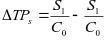
\includegraphics[width=0.8\textwidth]{assets/341}
	\caption*{}
\end{figure}- инвестицияның жиынтық табысқа
қатынасының өзгеру әсерінен экономикалық өсу қарқынының өзгеруі;

\begin{figure}[H]
	\centering
	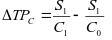
\includegraphics[width=0.8\textwidth]{assets/342}
	\caption*{}
\end{figure}- капитал сыйымдылығының өзгеру
әсерінен экономикалық өсу қарқынының өзгеруі;

\begin{figure}[H]
	\centering
	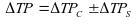
\includegraphics[width=0.8\textwidth]{assets/343}
	\caption*{}
\end{figure}- факторлардың өзгеру әсерінен
экономикалық өсу қарқынының жалпы өзгеруі.

{\bfseries Нәтижелер және талқылау.} 2018-2022 жылдар аралығында Ақмола
облысында жүзеге асырылған МЖӘ жобаларының саны туралы ақпараттар
1-суретте келтірілген:

{\bfseries 1-сурет. 2018-2022 жылдарғы Ақмола облысы бойынша жүзеге
асырылған МЖӘ жобаларының саны}

\emph{Ескерту - {[}4{]} әдебиеттен алынған мәліметтер негізінде
авторлармен құрастырылған}

1-суретке сәйкес Ақмола облысында 2018-2022 жылдар аралығында барлығы 66
МЖӘ жобасы жүзеге асырыла бастаған, ең көп жоба 2018 жылға тиесілі және
одан кейінгі жылдары күрт азайғандығын көруге болады. Сонымен жүзеге
асырылған жобалардың үлесі 2018 жылы -- 38,81\%, 2019 жылы -- 16,42\%,
2020 жылы -- 16,42\%, 2021 жылы -- 14,92\%, 2022 жылы - 11,94\% құраған.

МЖӘ жобалары әр түрлі салаларды қамтыған. Ең көбі білім беру саласында
-54 жоба, денсаулық сақтау -- 6 жоба, энергетика және тұрғын үй
коммунальдық шаруашылығы -- 1 жоба, көлік және инфрақұрылым -- 4 жоба,
ауылшаруашылығында -- 1 жоба нақты іске асырылып жатыр. Нақты іске
асырылып жатқан жобалардың экономика салалары бойынша үлесі де анықталды
және салалар бойынша үлесі келесі 2-суретте берілген:

{\bfseries 2-сурет. Ақмола облысы бойынша МЖӘ жобаларының құрылымы}

\emph{Ескерту - {[}4{]} әдебиеттен алынған мәліметтер негізінде
авторлармен құрастырылған}

2-суретке сәйкес МЖӘ жобаларының ішінде білім беру саласы бойынша
жасалған жобалардың үлесі - 82\%, денсаулық сақтау саласы - 9\%,
энергетика және тұрғын үй коммунальдық шаруашылығы саласы -- 2\%, көлік
және инфрақұрылым саласы - 6\% және ауыл, орман және балық шаруашылығы
саласы - 1\% құрап отыр. МЖӘ жобалары бойынша ең көп келісім-шарт
жасалған сала білім беру саласы, өйткені республика деңгейінде мектепке
дейінгі білім беру мәселесі өте өзекті болған еді. МЖӘ арқылы
балабақшалар жұмысын тиімді ұйымдастыруға жеке бизнес өкілдері белсенді
араласып, балабақша тапшылығын толықтай жойды.

Әрі қарай Ақмола облысының экономикалық өсу қарқынына талдау жасалды
және нәтижесі келесі 1-кесте берілген.

{\bfseries 1 - кесте. 2018-2022 жылдарғы Ақмола облысының экономикалық өсу
қарқыны}

\begin{longtable}[]{@{}
  >{\raggedright\arraybackslash}p{(\columnwidth - 12\tabcolsep) * \real{0.2991}}
  >{\raggedright\arraybackslash}p{(\columnwidth - 12\tabcolsep) * \real{0.1127}}
  >{\raggedright\arraybackslash}p{(\columnwidth - 12\tabcolsep) * \real{0.1030}}
  >{\raggedright\arraybackslash}p{(\columnwidth - 12\tabcolsep) * \real{0.1029}}
  >{\raggedright\arraybackslash}p{(\columnwidth - 12\tabcolsep) * \real{0.1029}}
  >{\raggedright\arraybackslash}p{(\columnwidth - 12\tabcolsep) * \real{0.1029}}
  >{\raggedright\arraybackslash}p{(\columnwidth - 12\tabcolsep) * \real{0.1765}}@{}}
\toprule\noalign{}
\begin{minipage}[b]{\linewidth}\raggedright
Көрсеткіштер
\end{minipage} & \begin{minipage}[b]{\linewidth}\raggedright
2018
\end{minipage} & \begin{minipage}[b]{\linewidth}\raggedright
2019
\end{minipage} & \begin{minipage}[b]{\linewidth}\raggedright
2020
\end{minipage} & \begin{minipage}[b]{\linewidth}\raggedright
2021
\end{minipage} & \begin{minipage}[b]{\linewidth}\raggedright
2022
\end{minipage} & \begin{minipage}[b]{\linewidth}\raggedright
Орташа өсу қарқыны, \%
\end{minipage} \\
\midrule\noalign{}
\endhead
\bottomrule\noalign{}
\endlastfoot
ЖӨӨ өсу қарқыны & 109,5 & 113,7 & 118,1 & 117,3 & 125,3 & 116,78 \\
ЖӨӨ өсім қарқыны & 9,5 & 13,7 & 18,1 & 17,3 & 25,3 & 16,78 \\
Өнеркәсіптік өндіріс көлемінің өсім қарқыны & 23,2 & 17,5 & 19,9 & 31,5
& 9,5 & 20,32 \\
\multicolumn{7}{@{}>{\raggedright\arraybackslash}p{(\columnwidth - 12\tabcolsep) * \real{1.0000} + 12\tabcolsep}@{}}{%
\emph{Ескерту - {[}4{]} әдебиеттен алынған мәліметтер негізінде
авторлармен құрастырылған}} \\
\end{longtable}

1-кестеге сәйкес 2018-2022 жылдары аралығында Ақмола облысының
экономикалық өсу қарқыны орташа есеппен 116,78\%, орташа өсім қарқыны
16,78\% және өнеркәсіптік өндіріс көлемі орташа өсім қарқыны 20,32\%
құраған. ЖӨӨ өсім қарқының құлашы 15,8\% құраған. Ең жоғарғы өсім
қарқыны 2022 жылы 25,3\% құраған және ең төменгі өсім қарқыны 2018 жылы
9,5\% құраған. Өнеркәсіптік өндіріс көлемінің ең жоғарғы өсім қарқыны
2021 жылы - 31,5\% өскен болса, ең төменгі өсім қарқыны 2022 жылы --
9,5\% өскенін көруге болады. Бұл көрсеткіштің 2018-2020 жылдар
аралығында кемігендігін байқауға болады.

Р. Харрод пен Е. Домар моделі бойынша экономиканың өсу қарқынына
талдауға қажетті мәліметтердің орташа абсолюттік өсімі есептелді және
талдау нәтижесі 2-кестеде берілген.

{\bfseries 2 - кесте. 2018-2022 жылдарғы Ақмола облысының экономикалық өсу
қарқынын сипаттайтын көрсеткіштердің орташа абсолютті өсімі}

\begin{longtable}[]{@{}
  >{\raggedright\arraybackslash}p{(\columnwidth - 12\tabcolsep) * \real{0.3508}}
  >{\raggedright\arraybackslash}p{(\columnwidth - 12\tabcolsep) * \real{0.0805}}
  >{\raggedright\arraybackslash}p{(\columnwidth - 12\tabcolsep) * \real{0.0933}}
  >{\raggedright\arraybackslash}p{(\columnwidth - 12\tabcolsep) * \real{0.0933}}
  >{\raggedright\arraybackslash}p{(\columnwidth - 12\tabcolsep) * \real{0.0933}}
  >{\raggedright\arraybackslash}p{(\columnwidth - 12\tabcolsep) * \real{0.1077}}
  >{\raggedright\arraybackslash}p{(\columnwidth - 12\tabcolsep) * \real{0.1812}}@{}}
\toprule\noalign{}
\begin{minipage}[b]{\linewidth}\raggedright
Көрсеткіштер
\end{minipage} & \begin{minipage}[b]{\linewidth}\raggedright
2018
\end{minipage} & \begin{minipage}[b]{\linewidth}\raggedright
2019
\end{minipage} & \begin{minipage}[b]{\linewidth}\raggedright
2020
\end{minipage} & \begin{minipage}[b]{\linewidth}\raggedright
2021
\end{minipage} & \begin{minipage}[b]{\linewidth}\raggedright
2022
\end{minipage} & \begin{minipage}[b]{\linewidth}\raggedright
Орташа абсолюттік өсім
\end{minipage} \\
\midrule\noalign{}
\endhead
\bottomrule\noalign{}
\endlastfoot
Негізгі капитал, млрд тг & 145,3 & 1619,3 & 1481,5 & 1683,8 & 2162,8 &
1418,54 \\
Өндірілген өнімнің көлемі, млрд тг & 536,4 & 553,3 & 686,4 & 827 &
1~542, 2 & 650,78 \\
Жиынтық табыс, млрд тг & 230,4 & 332 & 516,3 & 484,7 & 1~936,6 &
390,85 \\
Негізгі капиталға жасалған инвестициялар, млрд тг & 278,1 & 333,7 &
436,6 & 514, 6 & 566,5 & 403,73 \\
\multicolumn{7}{@{}>{\raggedright\arraybackslash}p{(\columnwidth - 12\tabcolsep) * \real{1.0000} + 12\tabcolsep}@{}}{%
\emph{Ескерту - {[}4{]} әдебиеттен алынған мәліметтер негізінде
авторлармен құрастырылған}} \\
\end{longtable}

2-кесте бойынша 2018-2022 жылдар аралығында Ақмола облысы бойынша
экономикалық өсу қарқынын сипаттайтын көрсеткіштердің орташа абсолюттік
өсімі мынаны көрсетті: негізгі капитал -- 1418,54 млрд тг, өндірілген
өнімнің көлемі -- 650,78 млрд тг, жиынтық табыс -- 390,85 млрд тг,
негізгі капиталға жасалған инвестициялар -- 403,73 млрд тг өскен.

Осы көрсеткіштер бойынша Р. Харрод пен Е. Домар моделі негізінде
2018-2022 жылдар аралығында Ақмола облысының экономикалық өсу қарқынына
талдау жасалды және талдау нәтижесі келесі 3-кестеде көрсетілген.

{\bfseries 3 - кесте. 2018-2022 жылдарғы Ақмола облысының экономиканың өсу
қарқынын Р. Харрод пен Е. Домар моделі бойынша талдау}

\begin{longtable}[]{@{}
  >{\raggedright\arraybackslash}p{(\columnwidth - 12\tabcolsep) * \real{0.3947}}
  >{\raggedright\arraybackslash}p{(\columnwidth - 12\tabcolsep) * \real{0.0937}}
  >{\raggedright\arraybackslash}p{(\columnwidth - 12\tabcolsep) * \real{0.0881}}
  >{\raggedright\arraybackslash}p{(\columnwidth - 12\tabcolsep) * \real{0.0882}}
  >{\raggedright\arraybackslash}p{(\columnwidth - 12\tabcolsep) * \real{0.0881}}
  >{\raggedright\arraybackslash}p{(\columnwidth - 12\tabcolsep) * \real{0.0882}}
  >{\raggedright\arraybackslash}p{(\columnwidth - 12\tabcolsep) * \real{0.1591}}@{}}
\toprule\noalign{}
\begin{minipage}[b]{\linewidth}\raggedright
Көрсеткіштер
\end{minipage} & \begin{minipage}[b]{\linewidth}\raggedright
2018
\end{minipage} & \begin{minipage}[b]{\linewidth}\raggedright
2019
\end{minipage} & \begin{minipage}[b]{\linewidth}\raggedright
2020
\end{minipage} & \begin{minipage}[b]{\linewidth}\raggedright
2021
\end{minipage} & \begin{minipage}[b]{\linewidth}\raggedright
2022
\end{minipage} & \begin{minipage}[b]{\linewidth}\raggedright
Орташа өсу қарқыны
\end{minipage} \\
\midrule\noalign{}
\endhead
\bottomrule\noalign{}
\endlastfoot
Инвестицияның жиынтық табысқа қатынасы, S & 1,21 & 1,01 & 0,85 & 1,06 &
0,29 & 0,88 \\
Капитал сыйымдылығы, C & 2,71 & 2,93 & 2,16 & 2,04 & 1,40 & 2,25 \\
Экономиканың өсу қарқыны, ТР & 0,45 & 0,34 & 0,39 & 0,52 & 0,21 &
0,38 \\
Экономиканың өсу қарқыны, ТР, \% & 44,6 & 34,4 & 39,2 & 52,2 & 20,9 &
38,26 \\
\multicolumn{7}{@{}>{\raggedright\arraybackslash}p{(\columnwidth - 12\tabcolsep) * \real{1.0000} + 12\tabcolsep}@{}}{%
\emph{Ескерту - {[}4{]} әдебиеттен алынған мәліметтер негізінде
авторлармен құрастырылған}} \\
\end{longtable}

3-кестеге сәйкес 2018-2022 жылдарғы Ақмола облысының экономиканың өсу
қарқынын Р. Харрод пен Е. Домар моделі бойынша мынаны көрсетті:
инвестицияның жиынтық табысқа қатынасы орташа есеппен 0,88 млн тг,
капитал сыйымдылығы 2,25 млн тг, экономиканың өсу қарқыны 0,38 немесе
38,26\% өскен.

Бұдан әрі экономикалық өсуді сипаттайтын көрсеткіштерге факторлық талдау
жасалды және нәтижесі келесі 4-кестеде берілген:

{\bfseries 4 - кесте. 2018-2022 жылдарғы Ақмола облысының экономиканың өсу
қарқынын Р. Харрод пен Е. Домар моделі бойынша факторлық талдау}

\begin{longtable}[]{@{}
  >{\raggedright\arraybackslash}p{(\columnwidth - 12\tabcolsep) * \real{0.2150}}
  >{\raggedright\arraybackslash}p{(\columnwidth - 12\tabcolsep) * \real{0.1208}}
  >{\raggedright\arraybackslash}p{(\columnwidth - 12\tabcolsep) * \real{0.1208}}
  >{\raggedright\arraybackslash}p{(\columnwidth - 12\tabcolsep) * \real{0.1359}}
  >{\raggedright\arraybackslash}p{(\columnwidth - 12\tabcolsep) * \real{0.1208}}
  >{\raggedright\arraybackslash}p{(\columnwidth - 12\tabcolsep) * \real{0.1208}}
  >{\raggedright\arraybackslash}p{(\columnwidth - 12\tabcolsep) * \real{0.1660}}@{}}
\toprule\noalign{}
\begin{minipage}[b]{\linewidth}\raggedright
Факторлар
\end{minipage} & \begin{minipage}[b]{\linewidth}\raggedright
2018
\end{minipage} & \begin{minipage}[b]{\linewidth}\raggedright
2019
\end{minipage} & \begin{minipage}[b]{\linewidth}\raggedright
2020
\end{minipage} & \begin{minipage}[b]{\linewidth}\raggedright
2021
\end{minipage} & \begin{minipage}[b]{\linewidth}\raggedright
2022
\end{minipage} & \begin{minipage}[b]{\linewidth}\raggedright
Орташа мәні
\end{minipage} \\
\midrule\noalign{}
\endhead
\bottomrule\noalign{}
\endlastfoot
1 фактор & -0,075 & -0,075 & -0,054 & 0,100 & -0,378 & -0,096 \\
2 фактор & 0,018 & -0,028 & 0,103 & 0,030 & 0,065 & 0,038 \\
Жалпы өзгерісі & 0,093 & -0,102 & 0,048 & 0,130 & -0,313 & -0,029 \\
\multicolumn{7}{@{}>{\raggedright\arraybackslash}p{(\columnwidth - 12\tabcolsep) * \real{1.0000} + 12\tabcolsep}@{}}{%
\emph{Ескерту - {[}4{]} әдебиеттен алынған мәліметтер негізінде
авторлармен құрастырылған}} \\
\end{longtable}

4-кесте бойынша 2018-2022 жылдар аралығында Ақмола облысының
экономикалық өсуі факторлардың өзгеру әсерінен орташа есеппен -0,096 млн
тг азайған, соның ішінде инвестицияның жиынтық табысқа қатынасының азаюы
әсерінен 0,038 млн тг және капитал сыйымдылығының азаюы әсерінен 0,029
млн тг азайған.

Өңірлік экономиканың негізгі және дәстүрлі әдістерінің бірі - өңірлердің
әлеуметтік-экономикалық дамуын талдау. Талдаудың мақсаты -
әлеуметтік-экономикалық даму стратегиясында қарастырылған экономикалық
өсуді негіздеу үшін сәйкессіздіктер мен пайдаланылмаған мүмкіндіктерді
анықтау болып табылады. Осы тұрғыда біздің зерттеу Ақмола облысының
экономикалық дамуына МЖӘ әсерін анықтау болып табылады. Экономикалық
дамуды сипаттау үшін экономикалық өсу коэффициенті қолданылды. 2018-2022
жылдар аралығында Ақмола облысының экономикалық өсуі келесі 4-суретте
көрсетілген:

{\bfseries 3 - сурет. 2018-2022 жылдары Ақмола облысының экономикалық өсуі}

\emph{Ескерту - {[}4{]} әдебиеттен алынған мәліметтер негізінде
авторлармен құрастырылған}

3-суретке сәйкес 2018-2022 жылдары Ақмола облысының экономикалық өсуі
0,45-0,21\% аралығын көрсетеді және жылдан жылға біртіндеп азайған.
Сондай-ақ инвестицияның жиынтық табысқа қатынасы 2,71-1,4 млн тг,
капитал сыйымдылығы 1,21-0,21 млн тг азайған.

2018-2022 жылдар аралығында Ақмола облысы бойынша жүзеге асырылған МЖӘ
жобаларынан тартылған инвестиция көлемі мен оның үлесі туралы келесі
3-суретте берілген:

{\bfseries 4 - сурет. 2018-2022 жылдарғы Ақмола облысы бойынша жүзеге
асырылған МЖӘ жобаларынан тартылған инвестиция көлемі мен үлесі}

\emph{Ескерту - {[}4{]} әдебиеттен алынған мәліметтер негізінде
авторлармен құрастырылған}

4-суретке сәйкес Ақмола облысында 2018-2022 жылдар аралығында барлығы
7783,26 мың теңге көлемінде инвестиция тартты және осы жылдар аралығында
тартылған инвестициялар орташа есеппен 15,36\% үлесті құрады. МЖӘ
жобаларынан тартылған инвестиция 2020 жылдан кейін күрт азайып
кеткендігін көреміз, себебі короновирустан кейінгі жағдай қаржылық
тапшылыққа алып келгені бір жағынан, 2020 жылға дейін қаржылық жабылуға
қол жеткізген жобалардың болуы екінші жағынан әсер етті. Сонымен
жобалардан тартылған инвестициялар көлемі мен үлесі 2018 жылы -- 1759,29
мың тг немесе 17,35\%, 2019 жылы -- 1477,35 мың теңге немесе 16,42\%,
2020 жылы -- 4471,65 мың теңге немесе 44,11\%, 2021 жылы -- 21 мың теңге
немесе 0,21\%, 2022 жылы -- 54 мың теңге немесе 0,54\% құраған.

Жалпы Ақмола облысының экономикалық даму деңгейі 2020 жылдан кейін күрт
төмендеген және сәйкесінше МЖӘ тартылған инвестиция да, жалпы
инвестицияда азайғанын көреміз. Оның негізгі себебі короновирус
кезеңінен кейінгі экономикалық құлдырау екендігімен түсіндіруге болады.

{\bfseries Қорытынды.} МЖӘ жобалары өңірдің экономикасын
диверсификациялауға және өсуіне ықпал етеді. Жаңа жобалар, әсіресе
инфрақұрылымдық жобалар, бизнесті дамытуға және экономикалық
белсенділікті арттыруға мүмкіндік береді. Өңірдің
әлеуметтік-экономикалық дамуын қамтамасыз ету үшін МЖӘ арқылы әлеуметтік
маңызы бар жобаларды іске асыруға болады. Ақмола облысында МЖӘ жобаларын
2018 жылдан бастап сәтті жүзеге асыруда. Соңғы жылдары іске асырылған
МЖӘ жобалары туралы сандық ақпаратты экономикалық-статистикалық
талдаумен бағалау, атап айтқанда, экономиканың қандай секторларында
жобалар іске асырылатынын, МЖӘ қандай түрін шаруашылық жүргізуші
субъектілер жиі пайдаланатынын, ұлттық деңгеймен салыстырғанда қанша
инвестиция тартылғанын бағалау және нәтижелерді талқылау орындалды.
Талдау нәтижесі бойынша мынандай қорытынды жасауға болады:

\begin{enumerate}
\def\labelenumi{\arabic{enumi}.}
\item
  Ақмола облысы бойынша барлығы 78 жоба ұсынылған, оның 66 нақты жүзеге
  асырыла бастаған, яғни әзірленген жобалардың 68,4\% жүзеге асырылды
  дегенді білдіреді. Бұл Ақмола өңірі бойынша МЖӘ жобаларын әзірлеу және
  жүзеге асыру белсенділігін көрсетеді.
\item
  Жобаларды жүзеге асырудың динамикасына жүргізілген талдау бойынша 2018
  жылы жүзеге асырылған жобалардың абсолюттік өсімі 21 жобаға немесе 3.5
  есеге өскенін байқауға болады. 2018 жылы жобалар саның өсуінің негізгі
  себебі балабақша мәселесінің өзекті болуына байланысты мектепке
  дейінгі білім беру орталықтарын құру бойынша жобалар жүзеге асырылды.
  Оған мемлекет қатты көңіл бөлді. Сөйтіп МЖӘ арқылы балабақша мәселесі
  шешілді. Ал 2020 жылы жобалар үлесі 27.3\% кеміген. Оның негізгі
  себебі жаппай короновирустың таралуына байланысты МЖӘ жобаларын
  конкурстан өткізу мәселелері туындады және жеке бастамашылдыққа
  басымдылық беру нәтижесінде жүзеге асырылатын жобалар саны күрт азайып
  кетті.
\item
  Ақмола облысы бойынша жүзеге асырылған жобалардың барлығы экономиканың
  мынандай бес саласын ғана қамтыған: транспорт және инфрақұрылым
  бойынша 6\%; білім беру -- 82\%; ауыл, орман және балық шаруашылығы --
  2\%; денсаулық сақтау -- 9\%; энергетика және тұрғын үй коммунальдық
  шаруашылығы -- 6\% құрап отыр. Жалпы Ақмола облысы аграрлықөңір
  болғандықтан ауыл, орман және балық шаруашылығы саласында жобаларды
  жүзеге асыруды көбейту керек.
\end{enumerate}

\begin{itemize}
\item
  Ақмола облысы бойынша МЖӘ сәтті жүзеге асыру үшін тұрақты
  инвестициялық климат құру қажет және оған әсер ететін мынандай
  факторларды ескеру қажет: үрдісті жүзеге асыру және алға жылжыту үшін
  мамандар қажет; үрдіске ықпал ететін заңнама; қаржылық қолдау.
\end{itemize}

4. 2018-2022 жылдары Ақмола облысының экономикалық өсуі 0,45-0,21\%
аралығын көрсетеді және жылдан жылға біртіндеп азайған. Сондай-ақ
инвестицияның жиынтық табысқа қатынасы 2,71-1,4 млн тг, капитал
сыйымдылығы 1,21-0,21 млн тг азайған.

Осы аталған ұсыныстарды ескерген жағдайда болашақта МЖӘ тиімді
пайдаланып өңірдің әлеуметтік-экономикалық мәселелерін шешуге мүмкіндік
береді.

{\bfseries Әдебиеттер}

\begin{enumerate}
\def\labelenumi{\arabic{enumi}.}
\item
  Regan M.,~Smith~J. Public infrastructure procurement: A review of
  adversarial and non-adversarial contracting methods // Journal of
  Public Procurement. -2015.~--Vol.15~(4). --P. 405-438.
  https://doi.org/10.1108/JOPP-15-04-2015-B001
\item
  Юрьева, Т. В. Государственно-частное партнерство в современной
  экономике: зарубежный опыт и российская практика // Статистика и
  экономика. -2013. -№ 6. --С. 127-130.
\item
  Қазақстан Республикасының Кәсіпкерлік Кодексі 2015 жылғы 29 қазандағы
  № 375-V (өзгерістер енгізілді-ҚР 03.07.2019 № 262-VI Заңымен).
  https://adilet.zan.kz/kaz/
\item
  База проектов. http://kzppp.kz/project\_base
\item
  Мемлекеттік-жекешелік әріптестік туралы Қазақстан Республикасының Заңы
  2015 жылғы 31 қазандағы № 379-V ҚРЗ.
  https://adilet.zan.kz/kaz/docs/Z1500000379
\item
  Герасименко О.А., Авилова Ж.Н., Осадчая С.М. Оценка эффективности
  региональных проектов государственно-частного партнерства // Вестник
  Белгородского университета кооперации, экономики и права. -2019.- № 1.
  - С. 102-109. https://doi.org/10.21295/2223-5639-2019-1-102-109
\item
  Mazharova L.A. Концептуальная модель оценки эффективности
  ГЧП-проектов. -2020.\\
  -Т.9. -№ 2. DOI:10.12731/2070-7568-2020-2-133-150
\item
  Berezin A, Bruno S, Gorodnova N. Efficiency Assessment of
  Public-Private Partnership (PPP) Projects: The Case of Russia.
  -Sustainability, 2018. --Vol. 10(10)
  https://doi.org/10.3390/su10103713
\item
  Peter E.D. Shared leadership, value and risks in large scale transport
  projects: Re-calibrating procurement policy for post COVID-19 //
  Research in Transportation Economics. -2020.
  https://doi.org/10.1016/j.retrec.2020.100999
\item
  Бакшеева, А. Д. Взаимодействия государства, бизнеса и образовательных
  организаций в рамках государственно-частного партнерства //
  Государственно-частное партнерство.\\
  -Т~3. -№ 1. -С 63-78. DOI:10.18334/ppp.3.1.35139
\item
  Verhoest, K., Petersen, O.H., Scherrer, W., Soecipto, R.M. How do
  governments support the development of public private partnerships?
  Measuring and comparing PPP governmental support in 20 European
  countries // Transport Reviews. -2015. --Vol. 35(2). --P. 118-139.
  DOI:10.1080/01441647.2014.993746
\item
  Wang, H., Liu, Y., Xiong, W., \& Zhu, D. (2019). Government support
  programs and private investments in PPP markets // International
  Public Management Journal. --Vol.~22(3). --P. 499-523.
  https://doi.org/10.1080/10967494.2018.1538025
\item
  Peer, N.O. Public Purpose Finance: The Government\textquotesingle s
  Role as Lender //Law \& Contemp. Probs. -2020. URL:
  https://scholarship.law.duke.edu/lcp/vol83/iss1/7
\item
  Wollmann, H. Verwaltungspolitische Strategie-und Politikwechsel im
  internationalen Vergleich: Zwischen Konvergenz und Divergenz //
  Gesellschaft mit beschränkter Hoffnung: Reformfähigkeit und die
  Möglichkeit rationaler Politik, Festschrift für Helmut Wiesenthal.
  -2004. -P. 116-144. https://doi.org/10.1007/978-3-322-80467-9\_6
\item
  Елисеев, А. В. Экономический рост в транзитивной экономике: дис. ...
  к.э.н.\\
  -Челябинск, 2003.--184 с.
\end{enumerate}

{\bfseries References}

1. Regan M., Smith J. Public infrastructure procurement: A review of
adversarial and non-adversarial contracting methods // Journal of Public
Procurement. -2015. --Vol.15 (4). --P. 405-438.
https://doi.org/10.1108/JOPP-15-04-2015-B001

2. Jur\textquotesingle eva, T. V. Gosudarstvenno-chastnoe partnerstvo v
sovremennoj jekonomike: zarubezhnyj opyt i rossijskaja praktika //
Statistika i jekonomika. -2013. -№ 6. --S. 127-130. {[}in Russian{]}

3. Qazaqstan Respýblıkasynyń Azamattyq Kodeksi 2015 jylǵy 29 qazandaǵy №
375-V (ózgerister týraly zań-QR 03.07.2019 № 262-VI Zańymen).
https://adilet.zan.kz/kaz/ {[}in Kazakh{]}

4. Baza proektov. http://kzppp.kz/project\_base {[}in Russian{]}

5. Memlekettik-jekeshelik áriptestik týraly qazaqstan Respýblıkasynyń
Zańy 2015 jylǵy 31 qazandaǵy № 379-V QRZ.
https://adilet.zan.kz/kaz/docs/Z1500000379 {[}in Kazakh{]}

6. Gerasimenko O.A., Avilova Zh.N., Osadchaja S.M. Ocenka jeffektivnosti
regional\textquotesingle nyh proektov gosudarstvenno-chastnogo
partnerstva // Vestnik Belgorodskogo universiteta kooperacii, jekonomiki
i prava. -2019.- № 1. - S. 102-109.
https://doi.org/10.21295/2223-5639-2019-1-102-109 {[}in Russian{]}

7. Mazharova L.A. Konceptual\textquotesingle naja
model\textquotesingle{} ocenki jeffektivnosti GChP-proektov. -2020. -T.
9. -№ 2. DOI:10.12731/2070-7568-2020-2-133-150 {[}in Russian{]}

8. Berezin A, Bruno S, Gorodnova N. Efficiency Assessment of
Public-Private Partnership (PPP) Projects: The Case of Russia.
-Sustainability, 2018. --Vol. 10(10) https://doi.org/10.3390/su10103713

9. Peter E.D. Shared leadership, value and risks in large scale
transport projects: Re-calibrating procurement policy for post COVID-19
// Research in Transportation Economics. -2020.
https://doi.org/10.1016/j.retrec.2020.100999

10. Baksheeva, A. D. Vzaimodejstvija gosudarstva, biznesa i
obrazovatel\textquotesingle nyh organizacij v ramkah
gosudarstvenno-chastnogo partnerstva // Gosudarstvenno-chastnoe
partnerstvo.

-T 3. -№ 1. -S 63-78. DOI:10.18334/ppp.3.1.35139 {[}in Russian{]}

11. Verhoest, K., Petersen, O.H., Scherrer, W., Soecipto, R.M. How do
governments support the development of public private partnerships?
Measuring and comparing PPP governmental support in 20 European
countries // Transport Reviews. -2015. --Vol. 35(2). --P. 118-139.
DOI:10.1080/01441647.2014.993746

12. Wang, H., Liu, Y., Xiong, W., \& Zhu, D. (2019). Government support
programs and private investments in PPP markets // International Public
Management Journal. --Vol. 22(3). --P. 499-523.
https://doi.org/10.1080/10967494.2018.1538025

13. Peer, N.O. Public Purpose Finance: The Government\textquotesingle s
Role as Lender //Law \& Contemp. Probs. -2020. URL:
https://scholarship.law.duke.edu/lcp/vol83/iss1/7

14. Wollmann, H. Verwaltungspolitische Strategie-und Politikwechsel im
internationalen Vergleich: Zwischen Konvergenz und Divergenz //
Gesellschaft mit beschränkter Hoffnung: Reformfähigkeit und die
Möglichkeit rationaler Politik, Festschrift für Helmut Wiesenthal.
-2004. -P. 116-144. https://doi.org/10.1007/978-3-322-80467-9\_6

15. Eliseev, A. V. Jekonomicheskij rost v tranzitivnoj jekonomike: dis.
... k.je.n. -Cheljabinsk, 2003.--184 s. {[}in Russian{]}

\emph{{\bfseries Авторлар туралы мәлімет}}

Рейдолда С. -«Экономика және қаржы» кафедрасының аға оқытушысы, магистр,
К.Кулажанов атындағы Казақ технология және бизнес университеті, Астана,
Казақстан, e-mail: Saulegul0408@gmail.com;

Бержанова А.М. -экономика ғылымдарының кандидаты, экономика және
кәсіпкерлік кафедрасының қауым. профессоры Л.Н. Гумилев атындағы Еуразия
Ұлттық Университеті, Астана, Қазақстан, e-mail:
aigul\_berjanova@list.ru;

Карпенко О.А. - Қаржы және несие кафедрасының доценті, РУДН, Мәскеу,
Ресей, e-mail: karpenko\_oa@rudn.university;

Садвоқасова К.Ж. - экономика ғылымдарының докторы, "Экономика және
қаржы" кафедрасының профессоры, Қ.Құлажанов атындағы қазақ Технология
және бизнес университеті, Астана, Қазақстан, e-mail: ksadvokas@mail.ru;

Жабытай Б.Н. - PhD, «Экономика және қаржы» кафедрасының қауымдастырылған
профессордың м.а, К.Кулажанов атындағы Казақ технология және бизнес
университет, Астана, Казақстан, e-mail: bayana\_7778@mail.ru;

Алпысбаева А.К.- экономика ғылыми кандидаты, «Экономика және қаржы»
кафедрасының қауымсыздырылған профессор (доцент) К.Кулажанов атындағы
Казақ технология және бизнес университет, Астана, Казақстан, e-mail:
alpysbayeva.ainur77@mail.ru

\emph{{\bfseries Information about the authors}}

Reidolda S. -Senior teacher of the Department of Economics and Finance,
K.Kulazhanov Kazakh University of Technology and Business, Astana,
Kazakhstan, e-mail: Saulegul0408@gmail.com;

Berzhanova A.M. -candidate of Economic Sciences, Аssociate professor of
the Department of Economics and entrepreneurship L.N. Gumilyov Eurasian
National University, Astana, Kazakhstan, e-mail:
aigul\_berjanova@list.ru; Karpenko O.A.- Аssociate professor of the
Department of Finance and Credit, RUDN, Moscow, Russian, e-mail:\\
karpenko\_oa@rudn.university;

Sadvokassova K. -doctor of economic sciences, professor of the
Department "Economics and finance", K.Kulazhanov Kazakh University of
Technology and Business, Astana, Kazakhstan, e-mail: ksadvokas@mail.ru;

Zhabytai B.N. -PhD, acting Associate Professor of the Department
Economics and Finance, K.Kulazhanov Kazakh University of Technology and
Business, Astana, Kazakhstan, e-mail: bayana\_7778@mail.ru;

Alpysbayeva A. -candidate of Economic Sciences, Аssociate professor of
the Department of Economics and Finance, K.Kulazhanov Kazakh University
of Technology and Business, Astana, Kazakhstan, e-mail:
alpysbayeva.ainur77@mail.ru\newpage
{\bfseries МРНТИ 06.75.03}

{\bfseries THE IMPACT OF FOREIGN AID ON THE ECONOMIC}

{\bfseries GROWTH OF CENTRAL ASIAN COUNTRIES}

(analytical review)

{\bfseries \textsuperscript{1}A.Serikkyzy, \textsuperscript{3}S.S.
Baktymbet\textsuperscript{🖂}, \textsuperscript{2}M. Ermirzoev,
\textsuperscript{1}A.B. Akhmetova}

\textsuperscript{1}ALMAU, Almaty, Kazakhstan,

\textsuperscript{2}University of Central Asia, Khorog, Republic of
Tajikistan,

\textsuperscript{3}Academy of Political Management, Astana, Kazakhstan

{\bfseries \textsuperscript{🖂}}Corresponding author: saule\_sbs@mail.ru

This study explores the relationship between foreign financial aid and
economic growth in Central Asian countries. Foreign aid is viewed as a
critical resource for promoting long-term growth by addressing key
challenges such as infrastructure, healthcare, and education. However,
the effectiveness of aid remains contentious, with critics arguing that
it may foster dependency, corruption, and inefficient use of resources.
Central Asia, comprising countries like Kazakhstan, Kyrgyzstan,
Uzbekistan, Tajikistan, and Turkmenistan, has received substantial
foreign financial aid since gaining independence following the
dissolution of the Soviet Union. While some scholars suggest that
foreign aid has positively impacted the economic growth of Central Asian
nations, others argue that it has had minimal or even negative effects.
This study emphasizes the importance of evaluating not only the amount
of aid but also its effectiveness, with a particular focus on the role
of institutional quality in determining the success of aid in promoting
sustainable economic development.

{\bfseries Key words:} foreign aid, economic growth, Central Asia,
dependence, corruption.

{\bfseries ВЛИЯНИЕ ИННОСТРАННЫХ ИНВЕСТИЦИЙ НА ЭКОНОМИЧЕСКИЙ РОСТ СТРАН
ЦЕНТРАЛЬНОЙ АЗИИ}

(аналитический обзор)

{\bfseries \textsuperscript{1}А.Серіккызы,
\textsuperscript{3}С.С.Бақтымбет\textsuperscript{🖂},
\textsuperscript{2}М.Eрмирзоев, \textsuperscript{1}А.Б.Ахметова}

{\bfseries \textsuperscript{1}}Университет ALMAU, Алматы, Казахстан,

{\bfseries \textsuperscript{2}}Университет Центральной Азии, г. Хорог,
Республика Таджикистан,

{\bfseries \textsuperscript{3}}Академия политического менеджмента, Астана,
Казахстан,

e-mail:saule\_sbs@mail.ru

В этом исследовании изучается взаимосвязь между иностранными
инвестициями и экономическим ростом стран Центральной Азии. Иностранные
инвестиций со стороны зарубежных государств рассматривается как
критически важный ресурс для содействия долгосрочному росту путем
решения таких ключевых задач, как инфраструктура, здравоохранение и
образование. Однако эффективность помощи остается спорной, поскольку
критики утверждают, что она может способствовать зависимости, коррупции
и неэффективному использованию средств. Центральная Азия, включающая в
себя такие страны, как Казахстан, Кыргызстан, Узбекистан, Таджикистан и
Туркменистан, получила значительную зарубежную финансовую помощь с
момента обретения независимости после распада Советского Союза. В этом
исследовании подчеркивается важность оценки не только количества помощи,
но и ее эффективности, с особым акцентом на роль институционального
качества в определении успеха помощи в содействии устойчивому
экономическому развитию.

{\bfseries Ключевые слова}: иностранные инвестиций, экономический рост,
Центральная Азия, зависимость, коррупция.

{\bfseries ШЕТЕЛДІК ИНВЕСТИЦИЯЛАРДЫҢ ОРТАЛЫҚ АЗИЯ ЕЛДЕРІНІҢ}

{\bfseries ЭКОНОМИКАЛЫҚ ӨСУІНЕ ӘСЕРІ}

(аналитикалық шолу)

{\bfseries \textsuperscript{1}А.Серікқызы, \textsuperscript{3}С.С.
Бақтымбет\textsuperscript{🖂}, \textsuperscript{2}М.Ермирзоев,}
{\bfseries \textsuperscript{1}А.Б. Ахметова}

\textsuperscript{1}Алматы менеджмент университеті ALMAU, Алматы,
Қазақстан,

\textsuperscript{2}Орталық Азия Университеті, Хорог, Тәжікстан
Республикасы,

\textsuperscript{3}Саяси менеджмент Академиясы, Астана, Қазақстан,

e-mail:saule\_sbs@mail.ru

Бұл зерттеу шетелдік қаржылық көмек пен Орталық Азия елдерінің
экономикалық өсуі арасындағы байланысты зерттейді. Шет мемлекеттердің
қаржылық көмегі инфрақұрылым, денсаулық сақтау және білім беру сияқты
негізгі міндеттерді шешу арқылы ұзақ мерзімді өсуге ықпал ететін маңызды
ресурс ретінде қарастырылады. Алайда, көмектің тиімділігі даулы болып
қала береді, өйткені сыншылар бұл тәуелділікке, сыбайлас жемқорлыққа
және қаражатты тиімсіз пайдалануға ықпал етуі мүмкін деп санайды.
Қазақстан, Қырғызстан, Өзбекстан, Тәжікстан және Түрікменстан сияқты
елдерді қамтитын Орталық Азия Кеңес Одағы ыдырағаннан кейін тәуелсіздік
алған сәттен бастап айтарлықтай шетелдік қаржылық көмек алды. Кейбір
ғалымдар шетелдік көмек Орталық Азия елдерінің экономикасының өсуіне оң
әсер етті деп болжаса, басқалары оның шамалы немесе тіпті теріс әсер
еткенін айтады. Бұл зерттеу көмектің мөлшерін ғана емес, оның
тиімділігін бағалаудың маңыздылығына баса назар аударады, бұл тұрақты
экономикалық дамуға көмектесудің сәттілігін анықтаудағы институционалдық
сапаның рөліне ерекше назар аударады.

{\bfseries Түйін сөздер}: шетелдік көмек, экономикалық өсу, Орталық Азия,
тәуелділік, жемқорлық.

{\bfseries Introduction.} The importance of understanding the relationship
between foreign investment and economic growth lies in shaping
appropriate development policies. Financial assistance is considered a
pivotal resource that adds to investment in the domestic country aimed
at long-term growth. It targets priority areas such as infrastructure,
healthcare, and education, which are essential for achieving sustainable
economic growth. At the same time, foreign aid can ensure stability and
act as a catalyst for implementing economic reforms during difficult
times. Despite this, the issue of the effectiveness of foreign aid in
promoting economic growth is widely debated; some authors who are
against foreign aid propose the statement that it can create dependence
and stimulate corruption. At the same time, it is possible that aid will
not be used for the intended purpose and will not directly support
economic policy due to the weak institutional quality. This study
examines foreign aid and economic growth in Central Asia.~

The Central Asian area is primarily comprised of five nations:
Kazakhstan, Kyrgyzstan, Uzbekistan, Tajikistan, and Turkmenistan. These
nations, which were republics of the Soviet Union, underwent significant
changes following the USSR's dissolution in 1991. Throughout this
period, they transitioned from a centrally planned economy to a
market-based economy. Although the transition process provided new
opportunities for growth and development, it caused these states to face
numerous obstacles and challenges.

Eventually, after gaining independence, the Central Asian states started
to receive a substantial amount of foreign aid. Most foreign assistance
came from donors, international organizations such as the World Bank,
International Monetary Fund, European Union, and developed nations,
including the United States, Japan, Germany, and other countries
contributing financially. The funds were intended to reduce the poverty
rate and achieve sustained growth.

Assessing the impact of international financial support on Central Asia
is important, yet this topic remains under debate. Some scholars believe
that foreign aid has a positive effect on growth, while other authors
claim that it does not have any effect or even negatively impacts the
economy. Proponents of aid state that it is essential for growth.
However, opponents of aid argue that it promotes reliance on foreign
funds and contributes to poor governance system or corruption when funds
are wasted. It is essential to analyze the impact of foreign monetary
assistance on economic expansion. Hence, it is important to analyze not
solely the amount of money received but also the efficiency of aid and
growth. Moreover, institutional quality is important because according
to the conventional wisdom higher institutional quality is associated
with the higher effectiveness of aid.

{\bfseries Definition of Aid.} It's worthwhile to mention that aid
encompasses different kinds of resources, such as tangible goods,
concessional loans, and nonrepayable financial grants. The Development
Assistance Committee (DAC) of the Organization for Economic Cooperation
and Development (OECD) represents the largest provider of aid,
consisting of 32 countries. The DAC defines aid as official development
assistance (ODA), which is primarily governmental aid designed for
developing countries\textquotesingle{} well-being and economic growth.
This organization has established specific criteria for identifying the
aid as ODA. First, it should come from the donor
country\textquotesingle s government agencies. The second criterion is
that it should achieve economic growth and contain a 25\% grant element
or more. Every three years, DAC updates its list of ODA receipts based
on the country\textquotesingle s per capita income. The DAC countries
expect recipient republics allocate development aid properly to mitigate
some of the economic challenges. Military aid and increased donor
security do not qualify as ODA. In some cases, aid for developing
countries can be in the form of humanitarian assistance, which includes
food and technical support such as projects or programs (OECD). For this
thesis, foreign aid specifically refers to the ODA.

{\bfseries Overview of Aid in Central Asia}{\bfseries .} As previously
mentioned, Central Asian countries began to receive foreign aid after
the collapse of the USSR. However, the countries did not receive the
same level of aid, and its distribution varied among them both in terms
of the amount received and the type of aid. For some developed
countries, providing foreign aid was a means of strengthening their
involvement in the region. Foreign aid from donor countries to Central
Asia mainly had a positive impact on the humanitarian, economic, and
social sectors of the economy. The DAC members directed most of the
foreign aid to the region. Notable China is not listed among these DAC
members, although it has been and continues to be one of the main
creditors for some Central Asian countries. Foreign aid, commonly
referred to as ODA (Official Development Assistance), primarily involves
the repayment of loans on concessional terms, such as the net repayment
of the principal and grant element, which includes at least 25\%,
estimated at a 10\% discount rate (OECD, 2024). From 2000 to 2020,
Central Asia received a total of \$11.57 billion in ODA from various
bilateral donors. Figure 1 below shows the distribution of ODA
throughout the region for the period 2000--2020.

{\bfseries Figure 1- Total ODA for Central Asia, 2000-2020 {[}1{]}.}

From figure 1, in 2011, Central Asia received the least amount of the
ODA, totalling \$412.38 million, and in 2019, the region received the
highest amount, \$931.28 million. Figure 2 displays the amount of ODA
receipts from 2000 to 2020.

{\bfseries Figure 2 - Net ODA classification by country {[}1{]}}

Uzbekistan leads in ODA receipts between 2000 and 2020, totaling \$4.3
billion. Following closely, Kyrgyzstan secures the second-highest amount
with \$2.82 billion. Notably, Kyrgyzstan was the first among Central
Asian countries to implement IMF policies. Tajikistan follows in third
place, having received \$2.52 billion. Uzbekistan takes the fourth spot,
with a net official ODA receipt of \$1.97 billion. Finally, Turkmenistan
concludes the list among Central Asian recipients, having received
\$227.8 million during the specified period.

{\bfseries Country Specific Trends}. Even though Central Asian countries
received different amounts of ODA from bilateral and multilateral
organizations throughout the period of 2000--2020, most of these states
had the same major donor. Next, the following subsection will describe
the ODA distribution for every Central Asian entity. It will mention the
prominent donors, the total amount of aid received, and the impact of
such aid on socioeconomic development.

{\bfseries Aid in Kazakhstan.}

{\bfseries Figure 3 - Main ODA providers for Kazakhstan, 2000-2020 {[}1{]}}

The USA is the largest ODA provider for Kazakhstan, offering \$1 billion
from 2000--2020. Like other donor countries, the USA targets specific
areas within Kazakhstan for its funds, including the social sector,
judiciary, and civil society. Additionally, it supports trade
opportunities and aids in the development of low-cost energy. Among
Central Asian countries, Kazakhstan allocates a sufficient budget to its
energy sector, with the US Agency for International Development (USAID)
actively supporting and promoting green energy policies {[}2{]}.

From 2000 to 2020, Kazakhstan received the highest amount of Official
Development Assistance (ODA) from Turkey. The Turkish Cooperation and
Coordination Agency's (TIKA) is an important aid provider focusing on
agricultural and livestock areas. In addition, TIKA supports the
improvement of social life standards through employment and vocational
training programs. Also, the agency supports the conservation of the
same historical and cultural identities {[}3{]}. This organization in
Kazakhstan also aims to improve the road infrastructure.

In 1997, Japan started to come up with Eurasian diplomacy, establishing
a political corporation with Kazakhstan and subsequently providing
investment in the energy sector. One of the highlighted projects between
Kazakhstan and Japan was the Silk Road Energy Mission. The "Central Asia
plus Japan" dialogue guided the project\textquotesingle s operation. The
aim of this project, accepted in 2006, was to enhance and promote atomic
energy safety and nuclear security. In essence, these two countries
share mutual benefits, particularly in the field of nuclear energy.
While Japan possesses advanced technology, it lacks some of its natural
resources, leading it to seek a high supply of uranium for its growing
nuclear energy sector. Kazakhstan, with the second-largest uranium
reserves, provides Japan with this resource. Cooperation agreements
between these countries primarily include investments in the nuclear
power industries, uranium mines, and technology exchange {[}4{]}.

Germany is the third country to strongly support Kazakhstan. During the
specified period, this country provided Kazakhstan with \$271.76
million. The GIZ organization directed the aid. Germany wants to
allocate its Official Development Assistance (ODA) to Kazakhstan for
education and sustainable economic development. This country, like the
United States, also allocates its ODA for training and employment
purposes. Additionally, Germany is concerned regarding environmental
challenges, public safety, and disaster prevention {[}5{]}.~

{\bfseries Aid in the Kyrgyz Republic.} Among Central Asian countries,
Kyrgyzstan was the first to adapt the IMF policies, which contributed to
receiving significant ODA since its independence. Countries like Japan,
Turkey, Germany, Switzerland, and international organizations like the
Asian Development Bank (Japan), the International Development
Assassination (IDA), and the United Nations (UN) are the main aid
providers for the Kyrgyz Republic. Figure 4 shows the main ODA providers
in Kyrgyzstan from 2000--2020.

{\bfseries Figure 4- Main providers of ODA for Kyrgyzstan, 2000-2020
{[}1{]}}

Although Russia is not included in the chart as the country was not
listed in the OECD database, it's noteworthy that the Russia began
providing financial assistance to Kyrgyzstan once they became part of
the Eurasian Economic Union (EEU). In 2015, Russia and the Kyrgyzstan
established a development fund containing \$1 billion. The main aim of
the Russia-Kyrgyz fund was to enhance the economic corporation between
these countries and modernize the Kyrgyz economy. According to the
Development aid report (2018) out of the \$1 billion, \$5000 million
were allocated from the Russian Federal Bank to the National Bank of
Kyrgyzstan. It should be mentioned that these ODA from the Russian fund
was not given for free; Kyrgyzstan will need to repay the loan later.
Top of Form.

Between 2000-2020, Turkey provided the Kyrgyzstan a total \$1169.52
million. The Turkish Cooperation and Coordination Agency (TIKA)
contributed significant amount of foreign aid to Kyrgyzstan, funding
over 760 distinct projects. TIKA wants its money in Kyrgyzstan to be
allocated for the education, infrastructure, and some portion for the
humanitarian purposes {[}6{]}.

USAID is considered one of the largest ODA providers for Kyrgyzstan.
During the mentioned period, the United States allocated \$1009.73
million to Kyrgyzstan. USAID primarily focuses on improving the
governance of the country. Additionally, the USA aims to develop and
promote the business environment and agriculture. Besides these
priorities, the USA also endeavours to positively contribute to various
sectors of the country, including education, healthcare, and human
rights {[}7{]}.

USAID is considered one of the largest ODA providers for Kyrgyzstan.
During the mentioned period, the United States allocated to the
Kyrgyzstan \$1.01 billion. USAID primarily focuses on improving the
governance of the country. Additionally, it promotes the business
environment and agriculture. In addition, the USA endeavors to make
positive contributions to various sectors, including human rights,
education, and healthcare {[}7{]}.

The Asian Development Bank (ADB) is a major multilateral organization
providing funds for Kyrgyzstan development. Between 2000 and 2020, it
allocated a total of \$444.14 million. Mainly ADB's support primarily
focuses on road's rehabilitation projects like Bishkek-Osh and the
Bishkek -Torugart routes, which connects the country's north and south
and link it with China {[}6{]}. Beside the road improvement in
Kyrgyzstan, ADB invests in various sectors such as education,
governmental structures, and the civil society. It also plays a
significant role in promoting water supply initiatives to facilitate
hydropower expansion. Notably, ADB undertook the rehabilitation of
Kyrgyzstan largest and most important power station of this country as
part of its project {[}7{]}.

Alongside with other international ODA providers, IDA stands out as a
major donor for Kyrgyzstan. From the period of 2000-2020 this
organization provided \$637.7 million in comprising both loans and
grants. IDA allocates its ODA towards the energy, agriculture, and
transportation initiatives {[}7{]}.

{\bfseries Aid in Tajikistan}. Like other Central Asian countries,
Tajikistan has also started to receive a significant amount of ODA since
its independence. Figure 5 illustrates the primary ODA allocation for
this country.

{\bfseries Figure 5- Main ODA providers Tajikistan 2000-2020 {[}1{]}}

From Figure 5, it's evident that ADB was Tajikistan\textquotesingle s
primary ODA provider between 2000 and 2020, contributing a total of
\$892.23 million. It began its collaboration with Tajikistan in 1998.
Initially, this country used ADB's funds for road construction. From
2005 to 2013, this organization facilitated the implementation of
Dushanbe-Kyrgyz Board Rehabilitation Project Phase 2. The ADB allocated
\$51.7 million for this project to improve and resurface the roads and
enhance the drainage systems, bridges, and walls {[}8{]}. This
organization had a significant and positive impact on the
country\textquotesingle s regional corporations and trade. Moreover, the
ADB projects led to the rehabilitation of three hydropower plants in
Tajikistan. In 2008, it allocated \$54.8 million for the ``Nurek 500
Kilovolt Switchyard Reconstruction Project {[}9{]}. Additionally, the
ADB directed its funds to enhance the country\textquotesingle s business
environment, social protection, tax policy, and finance system, while
also promoting employment through private partnerships, vocational
training, and food security promotion {[}10{]}.

From 2000 to 2020, USAID was Tajikistan\textquotesingle s second-highest
ODA provider. Primarily, USAID focuses on enhancing food security,
nutrition, and education while also aiming to improve institutional
quality. USAID strives to improve institutional quality by enhancing
government accountability, credibility, and oversight of basic services.
Moreover, it provides training and access to information for migrant
workers and civil society members. Additionally, this organization
places high value on human rights and tries to inform Tajikistan's
citizens about their rights {[}11{]}.

Tajikistan joined the International Development Association organization
in 1994, a year before joining the World Bank. The IDA directed its
funds towards mitigating climate risk and addressing natural disasters.
Additionally, this organization assists Tajikistan with electricity
exports and economic diversification {[}12{]}.

The European Union (EU) also aids Tajikistan. Primarily, the EU focuses
on three targets: rural development, education, and health. In
Tajikistan, the EU\textquotesingle s primary goal is to reduce poverty
in remote and rural areas by fostering inclusive economic activities in
agriculture and other sectors, thereby creating wealth and job
opportunities. Furthermore, like other international organizations, the
EU values sustainability and encourages the efficient use of natural
resources, as well as the enhancement of resilience to severe weather
conditions. Thanks to EU aid, Tajikistan greatly benefits, particularly
from projects promoting education, regional trade, and enhancing the
private sector and regional trade {[}13{]}.

{\bfseries Aid in Turkmenistan.} Among the central Asian countries,
Turkmenistan received the least amount of ODA. Figure 6 shows the
primary ODA providers in this country for the period 2000--2020.

{\bfseries Figure 6 - Main ODA providers for Turkmenistan, 2000-2020
{[}1{]}}

USAID is one of the largest ODA providers for Turkmenistan, with a total
of \$137.78 million. Like other Central Asian states, this organization
focuses on developing the health sector and youth initiatives in
Turkmenistan. Moreover, USAID assists local entrepreneurs by creating
different job opportunities and enhancing their competitiveness to
increase revenue. To foster citizens' trust in governmental
organizations, USAID promotes and encourages the use of e-governance
technologies, which positively impact information awareness and service
delivery {[}14{]}.

Another large donor for Turkmenistan is the United Arab Emirates (UAE),
which granted \$107.67 million. This country is one of Turkmenistan's
largest business partners, focusing on development corporations.
Infrastructure and road construction are areas of particular interest
for both states, including UAE and Turkmenistan. Additionally, they
prioritize areas such as science, education, culture, and heritage as
crucial components for developing and strengthening their relationship.

In total, the European Union provided \$74.66 million to Turkmenistan
from 2000 to 2020. This organization prioritizes its funds for
expenditure on public administrations and finances. Additionally, the EU
supports the country's private sector and agriculture, especially in
rural and remote areas. Moreover, this organization focuses on improving
the education system, addressing water and environmental problems, and
enhancing law enforcement. Finally, the EU endeavours to mitigate
political issues such as border management and assists in the training
of border guards {[}15{]}.

The United Nations Development Program (UNDP) operates prominently in
Turkmenistan, concentrating on achieving economic prosperity. Primarily,
this organization collaborates with partners to address social issues
such as human development, environmental sustainability, and energy
{[}16{]}.

{\bfseries Aid in Uzbekistan.}

{\bfseries Figure 7- Main ODA providers for Uzbekistan, 2000-2020 {[}1{]}}

Japan emerges as the largest aid provider for Uzbekistan for the period
of 2000-2020. Japan International Cooperation Agency (JICA) executes a
variety kind of initiatives including grants, concessional loans, and
the technical assistance. This organization allocates ODA towards
railroad projects, power generation, healthcare, agriculture, and other
sectors. A notable JICA program in Uzbekistan is the "Country Assistance
Policy to Uzbekistan ``established in 2012. It aims to stimulate
economic growth by addressing inequality and improving the economic
infrastructure {[}17{]}. Top of Form

In total Uzbekistan received \$1.74 billion from IDA, an agency under
the World Bank. The main aim of the provided ODA from the World Bank was
intended reducing poverty, achieving sustainable economic development,
improving the energy sector, and advancing market reforms. Overall, 28
projects of the World Bank are being implemented in Uzbekistan aiming to
rehabilitate irrigation and drainage system, improve the utility
infrastructure while fostering the economic growth of the country
{[}18{]}.

For the period of the 2000-2020 ADB provided to the Uzbekistan total
amount of the ODA \$7.6 million. Some part of this fund was directed
towards the development particularly for the electricity generation
projects. Under the Central Asian Regional Economic Cooperation (CAREC)
project, ADB in Uzbekistan supports road and railroad projects.
Additionally, ADB aided in providing access to clean water supply for
over 3 million people. Through the "Water Supply and Sanitation Services
Investment Program," more than 4,800 new households gained access to
clean water, and over 170,000 people were provided with improved sewage
services. ADB also assisted the agricultural sector, benefiting over 3.2
million individuals with water provision for agriculture and promoting
crop variety expansion and private sector engagement in horticultural
supply chains.Top of Form

Central Asian countries have benefited from the donor activities from
both DAC countries and international organizations. Major donors for
this region include Turkey, Japan, USA, and Germany while multilateral
organization such as ADB, USAID, IDA, and the EU also play a significant
role. The aim of DAC countries' assistance is mainly directed towards
the improvement of democracy and governance institutions. In Uzbekistan
and Kazakhstan, the focus of most aid is on improving the energy sector
while in Tajikistan and Turkmenistan a major portion of ODA is directed
towards transportation and the storage sector.

{\bfseries The Role of Specific ODA Providers to Central Asia}. Russia and
China are considered major~actors of the~``Eurasian''~and~``Shanghai
spirits''~for the economic development in Central Asia. These countries
are not part of the OECD, still these countries provide a significant
amount of ODA to the region.

{\bfseries Chinese Aid to Central Asia.} Even though China is not a part of
the DAC ODA providers, still it provides enough money to the Central
Asia through the programs like Belt and Road Initiative; It is worth
mentioning that China has a different definition and categorization of
the aid, which is broader than the one outlined by OECD. For example,
for China FDI, commercial loans are also considered as parts of the
foreign aid. Chinese aid is complex, and its statistics is released
through the governmental agencies. This country government set certain
rules based on which it provides it financial assistance to the rest of
the world. The following are eight principles based on which this
Chinese aid should be operated {[}19{]}.

\begin{enumerate}
\def\labelenumi{\arabic{enumi}.}
\item
  The aid provided by the Chinese government is based on the mutual
  benefits it has to the donor and the recipient. It is presented as a
  mutual exchange rather one-side charity.
\item
  The Chinese government does not place any conditions to the recipient
  country as they respect other country rules of law.
\item
  The aid is low-interest or free-interest loans that have the flexible
  repayment period.
\item
  The Chinese aid does not create the dependency but rather enables the
  recipient countries to achieve economic gains.
\item
  The Chinese assistance supports projects that require little spending
  but generate faster profits. This is because the success of such
  projects creates revenue for the recipient country and acquires
  capital.
\item
  The aid includes Chinese domestic machinery and if they fail to meet
  the agreed standard, China can replace them for free.
\item
  The Chinese government also enforces a high level of technical
  assistance to the recipient country and provides the recipient with
  its experts.
\item
  The Chinese experts sent for assistance to the recipient countries are
  expected to work under the same standards as local specialists.
\end{enumerate}

One of the papers devoted to the analysis of Chinese aid and its role in
Central Asia was written by Kashin and Korolev {[}20{]}. The authors of
this article underline the change in the vector of Chinese aid: from
being based on ideological driven agendas during the Cold war to more
economically focused objectives that mainly directed to the interests of
China as a whole.

Kashin and Korolev {[}20{]} also note that the in the past China
provided financial assistance to strengthen the position of Beijing role
in the world and overcome the international isolation. In addition, aid
from China has become one of the main tools to establish contacts with
the other countries.

Kashin and Korolev provide the critical assessment of the Chinese aid.
According to the authors despite the positive effect of Chinese aid to
the region, there might be some strategic motivation behind it. They
mention that even though Chinese aid in Central Asia promotes stability
and development, to some extend it is increasing its power to influence
the region. The authors state that the aid from China to Central Asia is
mostly aimed at infrastructure projects. One such example is the ``Silk
Road Economic Belt''. They argue that such projects not only support the
economic development of the region but also provides opportunity to
China to utilize its industrial capacity.

Authors mention that despite Chinese aid having its positive effects,
still some people believe that it raises concerns regarding becoming
dependent on it. For several years the inflow of Chinese capital to
Central Asia was directed toward infrastructure development which
further boosted the local economies and positively impacted the trade
relationships {[}20{]}.

The frame of China aid to Central Asia is based on the principles of the
mutual benefits of both parties. Mostly, a large amount of Chinese aid
in Central Asia is used for the economic infrastructure mainly the
construction of roads and extractive industries. Up to 2016, China has
granted Central Asia nearly \$30 billion dollars of concessional loans,
most of this amount was allocated to Kazakhstan and Turkmenistan
{[}20{]}.

Another paper about Chinese aid to the Central Asia was published by the
Nargiz Kassenova {[}21{]}. The study emphasizes the significance and
role of China's foreign aid to the region. According to her study
China's development assistance for the region also involves providing
buses, tractors, military supplies, and other kind of the equipment.
Additionally, China provides governmental scholarships to Central Asian
students and training programs for civil workers and military personnel.

Moreover, with both studies by Kassenova and Kashin and Korolev, China's
strategic use of its aid in Central Asia is questioned due to the
diverse objectives behind China's assistance. While Kashin and Korolev
argue that there has been a change to more economic variants from
ideologically driven agendas, they cannot deny the strategic motivation
on China's part. While the second article claims that the country's aid
is used to build strong social ties to the Central Asia. Both studies
explain mention about the goals of China's foreign aid within this
region, showcasing its economic aims in a broader sense.

{\bfseries Russian Aid to Central Asia.} Economically~Russia~has a dominant
influence in the energy sector, particularly~in countries like
Kazakhstan and Uzbekistan.~Additionally, Russia is interested in
some~sectors~like agriculture, construction, telecommunication,~and
mining.~Traditionally~Russian~aid to CA mainly focuses on region's
low-income countries~including~Tajikistan and Kyrgyzstan. In 2010,
Russian bilateral aid to Kyrgyzstan amounted \$25million.
Russia~provides its~aid~through the frameworks~such as the CIS and the
Economic Community.~According to the author~in~recent~years~Russia
forgave a significant amount of~aid~for Kyrgyzstan and Tajikistan for
securing the military cooperation~which~in total amounted~the~\$489
million {[}22{]}.

{\bfseries Conclusion.} Understanding the complex relationship between
foreign aid and economic growth is crucial for shaping effective
development policies, particularly in regions like Central Asia. While
foreign aid has the potential to drive long-term economic development by
addressing critical areas such as infrastructure, healthcare, and
education, its effectiveness remains a subject of debate. In Central
Asia, foreign assistance has played a significant role in the
post-Soviet transition period, with funds aimed at reducing poverty and
promoting sustained growth. However, concerns about aid dependency,
corruption, and inefficient use of funds persist. The impact of foreign
aid ultimately hinges on factors such as institutional quality, which
plays a pivotal role in determining the success of financial support in
fostering economic growth. Thus, a thorough evaluation of both the
quantity and the effectiveness of aid is essential to understanding its
true impact on the economic development of the region.

\emph{{\bfseries Financing}. This work was financially supported by the
Science Committee of the Ministry of Science and Higher Education of the
Republic of Kazakhstan (grant AP1968020, 2023--2025).}

{\bfseries References}

\begin{enumerate}
\def\labelenumi{\arabic{enumi}.}
\item
  OECD ODA trends and statistics. -2024. URL:
  https://www.oecd.org/en/topics/sub-issues/oda-trends-and-statistics.html
  (date of application - 12.09.2024)
\item
  Galante, A. How the U.S. benefits from foreign aid to Kazakhstan. The
  Borgen Project. -2018. URL:
  https://borgenproject.org/us-benefits-foreign-aid-kazakhstan/ (date of
  application - 12.09.2024)
\item
  Fidan, H., \& Nurdun, R. Turkey's role in the global development
  assistance community: the case of TIKA (Turkish International
  Cooperation and Development Agency) // Journal of Southern Europe and
  the Balkans. -2008. --Vol. 10(1). --P. 93--111.
  https://doi.org/10.1080/14613190801895888 (date of application
  12.09.2024)
\item
  Kassenova, T\& Toki, M. Japan and Kazakhstan: nuclear energy
  cooperation. The Nuclear Threat Initiative. -2010. URL:
  https://www.nti.org/analysis/articles/japan-kazakhstan-energy-cooperation/
  (date of application - 12.09.2022)
\item
  German Federal Foreign Office, Germany and Kazakhstan: Bilateral
  relations. -2024. URL:
  https://www.auswaertiges-amt.de/en/aussenpolitik/laenderinformationen/kasachstan-node/kazakhstan/218898
  (date of application - 12.09.2024)
\item
  Gunaydin, H. C. Turkey funded over 760 aid projects in Kyrgyzstan.
  Turkey (2018).
\item
  Development Aid. Donor activity in the Kyrgyz Republic: Special Report
  2018.
  https://events.developmentaid.org/attachment/ce1d8bd8-d82a-445a-a907-60db0b82f951/Kyrgyzstan\%20Report\%202018\%20-\%20Donor\%20Assistance\%20to\%20the\%20Kyrgyz\%20Republic.pdf
  Date of application - 12.09.2024
\item
  ADB Report Upgraded Tajikistan Road Improves Access to Markets. -2014.
  URL:
  https://www.adb.org/results/upgraded-tajikistan-road-improves-access-markets
  (date of application - 12.09.2024)
\item
  ADB Report Tajikistan Hydropower: Strengthening the Power Supply.
  -2014.
  https://www.adb.org/results/tajikistan-hydropower-strengthening-power-supply
  (date of application - 12.09.2024)
\item
  ADB Report Tajikistan Farmers Get Affordable Financing to Boost Food
  Supply. -2014. URL:
  https://www.adb.org/results/tajikistan-farmers-get-affordable-financing-boost-food-supply
  (date of application - 12.09.2024)
\item
  USAID (n.d). Agriculture and Food Security in Tajikistan. URL:
  https://www.usaid.gov/tajikistan/agriculture-and-food-security (date
  of application - 12.09.2024)
\item
  World Bank (n.d). Tajikistan - Energy Emergency Recovery Assistance
  Project (English). Washington, D.C: World Bank Group.
  http://documents.worldbank.org/curated/en/495351468133515937/Tajikistan-Energy-Emergency-Recovery-Assistance-Project
  (date of application - 12.09.2024)
\item
  European Commission (n.d). Tajikistan. URL:
  https://international-partnerships.ec.europa.eu/countries/tajikistan\_en
  (date of application - 12.09.2024)
\item
  USAID (n.d). USAID Turkmenistan. URL:
  https://www.usaid.gov/turkmenistan\#:\textasciitilde:text=In\%20Turkmenistan\%2C\%20USAID\%20advances\%20the,and\%20respect\%20for\%20human\%20rights\%3B
  (date of application - 12.09.2024)
\item
  European Union European Union and Turkmenistan. -2021.
  https://www.eeas.europa.eu/turkmenistan/european-union-and-turkmenistan\_en?s=231
  (date of application - 12.09.2024)
\item
  UNDP UNDP Turkmenistan. -2024. --URL:
  https://www.undp.org/turkmenistan (date of application - 12.09.2024)
\item
  JICA (n.d). Official Aid from Japan to Uzbekistan. URL:
  https://www.uz.emb-japan.go.jp/files/000224521.pdf (date of
  application - 12.09.2024)
\item
  Ibragimov M. The World Bank. The Government of Uzbekistan and the
  World Bank Affirm Their On-going Strategic Partnership. -2023. URL:
  https://www.worldbank.org/en/news/press-release/2023/03/11/the-government-of-uzbekistan-and-the-world-bank-affirm-their-on-going-strategic-partnership
  (date of application - 12.09.2024)
\item
  Information Office of the State Council. The People's Republic of
  China China's Foreign Aid. -2011. URL:
  http://en.cidca.gov.cn/2018-08/09/c\_261159.htm (date of application -
  12.09.2024)
\item
  Kashin V, Korolev A. Assistance of the PRC to the Central Asia
  countries. -2018. URL:
  https://publications.hse.ru/pubs/share/direct/218848124.pdf (date of
  application - 12.09.2024)
\item
  Kassenova N. How China's Foreign Aid Fosters Social Bonds With Central
  Asian Ruling Elites. -2022. URL:
  https://sites.tufts.edu/fletcherrussia/files/2023/01/Kassenova\_Chinese\_Aid\_Final.pdf
  (date of application - 12.09.2024)
\item
  Oliphant C. Russia's role and interest in Central Asia. -2013. URL:
  https://www.files.ethz.ch/isn/172941/russias-role-and-interests-in-central-asia.pdf.
\end{enumerate}

\emph{{\bfseries Information about authors}}

Serikkyzy A .- PhD, associate professor ALMAU, Almaty, Kazakhstan,
e-mail: a.serikkyzy@almau.edu.kz;

Baktymbet S. S.-candidate of Economic Sciences, Associate Professor,
Academy of Political Management, Astana, Kazakhstan, e-mail:
saule\_sbs@mail.ru;

Yermirzoev M. - candidate of Economic Sciences, Associate Professor of
the University of Central Asia, Khorog, Republic of Tajikistan, e-mail:
mirzobobo.yormirzoev@ucentralasia.org;

Akhmetova A.B. -- bachelor, ALMAU, Almaty, Kazakhstan, e-mail:
arsiapev@gmail.com

\emph{{\bfseries Сведения об авторах}}

Серіккызы А. - PhD, ассоциированный профессор ALMAU, Алматы, Казахстан,
e-mail: a.serikkyzy@almau.edu.kz;

Бақтымбет С.С. -- кандидат экономических наук, доцент, Академия
политического менеджмента, Астана, Казахстан, e-mail:
saule\_sbs@mail.ru;

Eрмирзоев М.- кандидат экономических наук, доцент Университета
Центральной Азии,Хорог, Республика Таджикистан, e-mail:
mirzobobo.yormirzoev@ucentralasia.org;

Ахметова А.Б. -- бакалавр, ALMAU, Алматы, Казахстан, arsiapev@gmail.com\newpage
{\bfseries МРНТИ 06.73.93}

{\bfseries СОВЕРШЕНСТВОВАНИЕ СИСТЕМЫ УЧЕТА И АНАЛИЗА ЗАТРАТ НА ОХРАНУ ТРУДА
В РЕСПУБЛИКЕ КАЗАХСТАН: ПРОБЛЕМЫ, ПЕРСПЕКТИВЫ И СТРАТЕГИИ УЛУЧШЕНИЯ}

{\bfseries \textsuperscript{1}А. М. Курманов, \textsuperscript{2}И.
Е.Сарыбаева\textsuperscript{🖂}, \textsuperscript{3}А. Н. Омаркожаева,
\textsuperscript{1}А.Б. Бекмагамбетов}

\textsuperscript{1} Республиканский научно-исследовательский институт по
охране труда Министерства труда и социальной защиты населения Республики
Казахстан, Астана, Казахстан,

\textsuperscript{2} Евразийский национальный университет имени Л.Н.
Гумилева, Астана, Казахстан,

\textsuperscript{3} Казахский университет технологии и бизнеса
им.К.Кулажанова, Астана, Казахстан

{\bfseries \textsuperscript{🖂}}Корреспондент-автор:
inarasaribaeva@gmail.com

В статье рассматриваются проблемы и перспективы совершенствования
системы социальных гарантий для работников, занятых на вредных и опасных
производствах в Республике Казахстан. На основе анализа текущего
законодательства и практики предоставления компенсаций выявлены
существенные недостатки, связанные с отсутствием единого подхода к
аттестации рабочих мест и недостаточной объективностью оценки условий
труда. Особое внимание уделяется необходимости разработки
унифицированных стандартов и критериев оценки, усилению контроля за
проведением аттестации, а также внедрению дифференцированного подхода к
предоставлению социальных гарантий. В статье предложены рекомендации по
совершенствованию системы, которые включают разработку новых
законодательных актов, повышение квалификации специалистов по охране
труда и создание механизмов обратной связи для работников. Эти меры
направлены на обеспечение более справедливых и равных условий труда, что
в конечном итоге способствует улучшению производственной среды и
снижению уровня профессиональных заболеваний.

{\bfseries Ключевые слова:} социальные гарантии, вредные и опасные условия
труда, компенсации, охрана труда, аттестация рабочих мест, условия труда

{\bfseries ҚАЗАҚСТАН РЕСПУБЛИКАСЫНДА ЕҢБЕКТІ ҚОРҒАУҒА АРНАЛҒАН ШЫҒЫНДАРДЫ
ЕСЕПКЕ АЛУ ЖӘНЕ ТАЛДАУ ЖҮЙЕСІН ЖЕТІЛДІРУ: ПРОБЛЕМАЛАР, ПЕРСПЕКТИВАЛАР
ЖӘНЕ ЖАҚСАРТУ СТРАТЕГИЯЛАРЫ}

{\bfseries \textsuperscript{1}А. М. Курманов, \textsuperscript{2}И. Е.
Сарыбаева\textsuperscript{🖂}, \textsuperscript{3}А. Н. Омарқожаева,
\textsuperscript{1}А.Б. Бекмағамбетов}

\textsuperscript{1} Қазақстан Республикасы Еңбек және халықты әлеуметтік
қорғау министрлігінің Еңбекті қорғау жөніндегі республикалық
ғылыми-зерттеу институты, Астана, Қазақстан,

\textsuperscript{2} Л. Н. Гумилев атындағы Еуразия Ұлттық Университеті,
Астана, Қазақстан,

\textsuperscript{3} Қазақ технология және бизнес университеті.Қ.
Құлажанова, Астана, Қазақстан,

e-mail: inarasaribaeva@gmail.com

Мақалада Қазақстан Республикасындағы зиянды және қауіпті өндірістерде
жұмыс істейтін қызметкерлер үшін әлеуметтік кепілдіктер жүйесін
жетілдіру мәселелері мен перспективалары қарастырылады. Ағымдағы
заңнаманы және өтемақы беру практикасын талдау негізінде жұмыс орындарын
аттестаттауға бірыңғай тәсілдің болмауына және еңбек жағдайларын
бағалаудың объективтілігінің жеткіліксіздігіне байланысты елеулі
кемшіліктер анықталды. Бірыңғай стандарттар мен бағалау критерийлерін
әзірлеу, аттестаттауды өткізуді бақылауды күшейту, сондай-ақ әлеуметтік
кепілдіктер беруге сараланған тәсілді енгізу қажеттілігіне ерекше назар
аударылады. Мақалада жаңа заңнамалық актілерді әзірлеуді, еңбекті қорғау
жөніндегі мамандардың біліктілігін арттыруды және қызметкерлер үшін кері
байланыс тетіктерін құруды қамтитын жүйені жетілдіру бойынша ұсыныстар
ұсынылған. Бұл шаралар неғұрлым әділ және тең еңбек жағдайларын
қамтамасыз етуге бағытталған, бұл сайып келгенде өндірістік ортаны
жақсартуға және кәсіптік аурулардың деңгейін төмендетуге ықпал етеді.

{\bfseries Негізгі сөздер:} әлеуметтік кепілдіктер, зиянды және қауіпті
еңбек жағдайлары, өтемақылар, еңбекті қорғау, жұмыс орындарын
аттестаттау, еңбек жағдайлары

{\bfseries IMPROVING THE SYSTEM OF ACCOUNTING AND ANALYSIS OF LABOR
PROTECTION COSTS IN THE REPUBLIC OF KAZAKHSTAN: PROBLEMS, PROSPECTS AND
IMPROVEMENT STRATEGIES}

{\bfseries \textsuperscript{1}A.M.Kurmanov, \textsuperscript{2}I.E.
Sarybayeva\textsuperscript{🖂} , \textsuperscript{3}A.N. Omarkozhayeva,
\textsuperscript{1}A.B.Bekmagambetov}

\textsuperscript{1} Republican Research Institute for labor protection
of the Ministry of Labor and social protection of the population of the
Republic of Kazakhstan, Astana, Kazakhstan,

\textsuperscript{2} L. N. Gumilyov Eurasian National University, Astana,
Kazakhstan,

\textsuperscript{3} K.Kulazhanov Kazakh University of Technology and
Business, Astana, Kazakhstan,

e-mail: inarasaribaeva@gmail.com

The article discusses the problems and prospects of improving the system
of social guarantees for workers employed in hazardous and hazardous
industries in the Republic of Kazakhstan. Based on the analysis of
current legislation and the practice of providing compensation,
significant shortcomings have been identified related to the lack of a
unified approach to workplace certification and insufficient objectivity
in assessing working conditions. Special attention is paid to the need
to develop unified standards and evaluation criteria, strengthen control
over certification, as well as introduce a differentiated approach to
the provision of social guarantees. The article offers recommendations
for improving the system, which include the development of new
legislative acts, professional development of occupational safety
specialists and the creation of feedback mechanisms for employees. These
measures are aimed at ensuring fairer and more equal working conditions,
which ultimately contributes to improving the working environment and
reducing occupational diseases.

{\bfseries Key words:} social guarantees, harmful and dangerous working
conditions, compensation, labor protection, certification of workplaces,
working conditions

{\bfseries Введение.} Вопросы исследования социальных гарантий для
работников, занятых на вредных производствах труда, являются крайне
важными и многоаспектными, что обусловлено в первую очередь обеспечением
благосостояния и защиты здоровья работников. На фоне развития
промышленности и внедрения новых производственных технологий, характер и
степень воздействия на здоровье работников также изменяются, что требует
пересмотра и обновления социальных гарантий. Кроме того, важным аспектом
является обеспечение справедливости и равенства в распределении таких
гарантий среди всех категорий работников, занятых на вредных
производствах. Это связано с необходимостью учета индивидуальных
факторов риска и особенностей различных отраслей.

В соответствии со статьей 181 Трудового кодекса РК {[}1{]} работник
имеет право на рабочее место, оборудованное в соответствии с
требованиями по безопасности и охране труда, обеспечение
санитарно-бытовыми помещениями, средствами индивидуальной и коллективной
защиты в соответствии с требованиями законодательства, а также трудовым,
коллективным договорами. А по статье 182 работодателю вменяется в
обязанность проведение постоянного мониторинга уровня профессиональных
рисков с целью его профилактики, а также замены применяемых опасных
технологий и производственного оборудования на более безопасные.

Несмотря на принятые новые законодательные акты {[}2,3{]} социальные
гарантии в Казахстане по-прежнему не соответствуют ожиданиям и
потребностям работников и не обеспечивают выполнение международных норм,
не учитывают современное состояние производства и производственной
среды, условия труда на рабочих местах.

Социальные гарантии играют важную роль в уменьшении неравенства,
вызванного различиями в условиях труда, и поддерживают социальное
равновесие. В условиях модернизации производственных процессов и
изменений в трудовом законодательстве возникает необходимость пересмотра
и адаптации социальных гарантий, чтобы они оставались эффективными и
актуальными в новых социально-экономических реалиях.

Таким образом, исследование социальных гарантий для работников, занятых
на вредных производствах труда, имеет ключевое значение для развития
социальной политики и охраны труда, а его результаты могут стать основой
для принятия более эффективных и справедливых решений в данной области.

{\bfseries Материалы и методы.} Темой исследования занимались и занимаются
до сих пор как отдельные ученые, так проектные организации,
научно-исследовательские институты. Большое число публикаций посвящены
вопросам охраны труда, но теме «совершенствование регулированию труда
работников вредного и опасного производства» посвящены единичные труды.
Более того, вся изученная литература является справочной, либо
теоретические работы посвящены, как правило, решению каких-либо
отдельных вопросов, так или иначе касающихся вопросов охраны и условий
труда.

Анализ действующего механизма регулирования труда лиц, занятых в
неблагоприятных условиях изучены как отечественными, так и зарубежными
специалистами. Среди российских работ можно отметить статьи А.М. Елина,
С.С. Сергеевой «Специальная оценка условий труда: практика и итоги»
{[}4{]}, Л.И. Хайруллина, В.С. Гасилова, Тучковой О.А. «Компенсации за
работу во вредных условиях труда: основные аспекты вопроса» {[}5{]},
С.М.Ильина, Н.А., Самарской и др. «Направления совершенствования системы
предоставления гарантий и компенсаций работникам за работу в опасных
(вредных) условиях труда» {[}6{]}. Подобные исследования проводятся
также учеными странами СНГ в частности, статья Стратулата В. И.
«Социальные компенсации за вредные условия труда в Молдове» {[}7{]},
Алиевой Л. М. «Компенсационные механизмы для работников во вредных
условиях труда в Азербайджане» {[}8{]}, Умарова Н. А. «Правовые аспекты
компенсации за вредные условия труда в Узбекистане» {[}9{]} и др. В
Казахстане можно отметить, следующие исследования С.Г. Бисакаева, Ш.К.
Абикеновой, Каминскаой Г. А. «Научное обоснование механизма
государственного регулирования труда работников, занятых во вредных
условиях труда» {[}10{]}, Г.А. Еселхановой, А.Е. Танабаевой
«Нормативно-правовое регулирование предоставления гарантий работникам,
занятым во вредных и опасных условиях труда в Республике Казахстан»
{[}11{]}, С.М. Базарбаевой, С.Т. Шорманова, С.Т. Толеугали «Анализ
действующего механизма регулирования труда лиц, занятых в
неблагоприятных условиях» {[}12{]}.

Можно отметить ряд работ ученых дальнего зарубежья Lee, H. S., Kim, J.
H. «Occupational hazards and safety management in the South Korean
manufacturing sector» (Южная Корея) {[}13{]}, Leigh, J. P., Du, J.
«Economic burden of occupational injuries and illnesses in the United
States» {[}14{]} (США), Pissarides, C. A., Weber, A. «Compensation for
workplace risks in the European Union: Evidence from the European
Working Conditions Survey» {[}15{]} (Европа) и др.

Таким образом, в данном исследовании использовались различные источники
и методы для анализа действующего механизма регулирования труда лиц,
занятых в неблагоприятных условиях. Характеристика исследовательского
материала включает в себя как качественные, так и количественные
аспекты, что является важным фактором для обеспечения достоверности
выводов и методов исследования.

Исследование проводилось в несколько этапов: анализ существующих
законодательных актов, сбор и анализ статистических данных по
численности работников, занятых во вредных условиях труда, и
сравнительный анализ компенсационных механизмов.

При написании статьи использовались следующие методы: документальный
анализ правовых актов, статистический анализ данных по численности
работников, занятых во вредных условиях труда, и их компенсации,
сравнительный анализ компенсаций по различным формам собственности
предприятий.

{\bfseries Результаты и обсуждение.} Социальная защита работников, занятых
на тяжелых работах, а также на работах с вредными и (или) опасными
условиями труда, является одной из важнейших задач государственной
политики в сфере трудовых отношений в Республике Казахстан.
Нормативно-правовое регулирование в этой области направлено на создание
условий, обеспечивающих здоровье и безопасность работников, а также на
предоставление им дополнительных социальных гарантий и компенсаций.

Нормативно-правовой анализ исследования регуляторных норм, действующих в
Республике Казахстан представлен в таблице 1.

{\bfseries Таблица 1 - Нормативно-правовой анализ регуляторных норм в сфере
охраны труда}

\begin{longtable}[]{@{}
  >{\raggedright\arraybackslash}p{(\columnwidth - 2\tabcolsep) * \real{0.3111}}
  >{\raggedright\arraybackslash}p{(\columnwidth - 2\tabcolsep) * \real{0.6889}}@{}}
\toprule\noalign{}
\begin{minipage}[b]{\linewidth}\raggedright
Нормативный акт
\end{minipage} & \begin{minipage}[b]{\linewidth}\raggedright
Основное содержание
\end{minipage} \\
\midrule\noalign{}
\endhead
\bottomrule\noalign{}
\endlastfoot
\multicolumn{2}{@{}>{\raggedright\arraybackslash}p{(\columnwidth - 2\tabcolsep) * \real{1.0000} + 2\tabcolsep}@{}}{%
Трудовой кодекс РК} \\
ст. 69 п. 2 & Устанавливается сокращенная продолжительность рабочего
времени не более 36 часов для работников, занятых на тяжелых и опасных
работах. \\
ст. 89 п. 1 & Предоставляются дополнительные оплачиваемые ежегодные
трудовые отпуска продолжительностью не менее шести календарных дней для
работников на тяжелых и опасных работах. \\
ст. 105 п. 1 & Оплата труда для работников на тяжелых и опасных работах
устанавливается в повышенном размере по сравнению с оплатой труда
работников с нормальными условиями труда. \\
ст. 182 п. 2 & Работодатель обязан создавать санитарно-гигиенические
условия, обеспечивать работников молоком или равноценными пищевыми
продуктами, специализированными продуктами для диетического питания. \\
\multicolumn{2}{@{}>{\raggedright\arraybackslash}p{(\columnwidth - 2\tabcolsep) * \real{1.0000} + 2\tabcolsep}@{}}{%
Социальный кодекс РК} \\
ст. 195-1 & Устанавливает право на социальную защиту для лиц, занятых на
работах с вредными условиями труда, при достижении 55-летнего возраста и
уплате обязательных профессиональных пенсионных взносов в совокупности
не менее 84 месяцев. \\
Постановление Правительства РК от 26.03.2014 г. № 255 & Об утверждении
Правил осуществления обязательных профессиональных пенсионных
взносов. \\
Закон Республики Казахстан "О внесении изменений и дополнений в
некоторые законодательные акты по вопросам общественных объединений и
социальной защиты лиц, занятых на работах с вредными условиями труда" &
Подписан Главой государства, включает новые выплаты и социальные
гарантии для работников на вредных работах\hspace{0pt}
(PRO1C)\hspace{0pt}\hspace{0pt} (PRO) \\
\multicolumn{2}{@{}>{\raggedright\arraybackslash}p{(\columnwidth - 2\tabcolsep) * \real{1.0000} + 2\tabcolsep}@{}}{%
Приказы Министерства здравоохранения и социального развития РК} \\
№ 1053 от 28.12.2015 г. & Об утверждении Списка производств, цехов,
профессий и должностей, перечня тяжелых и опасных работ, дающих право на
сокращенное рабочее время, дополнительный отпуск и повышенную оплату
труда. \\
№ 1054 от 28.12.2015 г. & Об утверждении Правил выдачи работникам молока
или равноценных пищевых продуктов, специализированных продуктов для
диетического питания, специальной одежды и других средств индивидуальной
защиты. \\
№ 1056 от 28.12.2015 г. & Об утверждении норм выдачи работникам молока
или равноценных пищевых продуктов, специализированных продуктов для
диетического питания. \\
Приказ Министерства труда и социальной защиты населения РК от 24.05.2023
г. № 170 & Об утверждении перечня производств, работ, профессий
работников, занятых на работах с вредными условиями труда, для которых
осуществляются обязательные профессиональные пенсионные взносы за счет
средств работодателя. \\
\multicolumn{2}{@{}>{\raggedright\arraybackslash}p{(\columnwidth - 2\tabcolsep) * \real{1.0000} + 2\tabcolsep}@{}}{%
Примечание -- составлено авторами на основании {[}1-3{]}} \\
\end{longtable}

Анализ данных, приведенных в таблице 1, показывает, что в Республике
Казахстан осуществляется комплексный подход к регулированию трудовых
отношений и предоставлению социальных гарантий для работников, занятых
на тяжелых и опасных работах. Принятие новых законодательных актов
направлено на улучшение условий труда и усиление социальной защиты
работников, что способствует созданию безопасных и здоровых условий
труда в стране.

В 2023 году численность работников, занятых во вредных и других
неблагоприятных условиях труда составляло 1 692~214 человек, что на
21065 человек больше в сравнении с 2022 годом и на 50621 человек больше
в сравнении с 2021 годом.

Вредные факторы труда оказывают значительное воздействие на здоровье и
работоспособность работников, что делает их изучение и регулирование
важной задачей для обеспечения безопасных и здоровых условий труда. В
условиях современной экономики, где значительное количество рабочих мест
связано с потенциально опасными производственными процессами, понимание
и минимизация вредных факторов является ключевым аспектом социальной
политики и трудового законодательства.

Воздействие вредных факторов проявляется на физическом, психологическом
и социальном уровнях. Физическое воздействие может привести к различным
заболеваниям и травмам, снижающим общую работоспособность работников.
Психологическое воздействие выражается в повышенном уровне стресса,
утомляемости и снижении когнитивных функций, что также негативно
сказывается на производительности труда. Социальное и экономическое
воздействие вредных факторов проявляется в снижении качества жизни
работников и экономических потерях, связанных с медицинскими расходами и
снижением эффективности труда (рисунок 1).

Наибольший удельный вес работающих во вредных условиях труда в 2023 году
зафиксировано в следующих секторах экономики:

\begin{itemize}
\item
  добыча угля - 75,6\%;
\item
  горнодобывающая промышленность и разработка карьеров - 53,0\%;
\item
  промышленность - 41,0\%;
\item
  снабжение электроэнергией, газом, паром, горячей водой и
  кондиционированным воздухом - 34,8\%.
\end{itemize}

Высокий удельный вес работающих во вредных условиях труда в этих
секторах обоснованы следующими факторами: усложненными технологическими
процессами, использованием тяжелого оборудования и взрывчатых веществ,
экстремальными температурами, воздействием токсичных веществ и др.
(рисунок 2)

Физическое воздействие

Заболевания и травмы. Вредные факторы, такие как шум, вибрация,
запыленность и загазованность воздуха, экстремальные температуры, могут
вызвать острые и хронические заболевания.

Снижение работоспособности. Воздействие вредных факторов может привести
к быстрой утомляемости, снижению физической выносливости и общей
работоспособности. Это, в свою очередь, повышает риск производственных
травм и аварий.

Психологическое воздействие

Стресс и утомляемость. Вредные факторы, такие как шум и вибрация, могут
вызывать повышенный стресс и утомляемость, что негативно сказывается на
психическом здоровье работников. Хронический стресс может привести к
развитию депрессии, тревожных расстройств и других психических
заболеваний.

Снижение концентрации и когнитивных функций. Шум и вибрация могут
снижать концентрацию внимания и когнитивные функции, что затрудняет
выполнение сложных и требующих внимания задач.

Социальное и экономическое воздействие

Снижение качества жизни. Хронические заболевания и психическое
напряжение, вызванные вредными факторами труда, могут снижать общее
качество жизни работников, ограничивая их физические и социальные
возможности.

Экономические потери. Заболевания и травмы работников приводят к потерям
рабочего времени, увеличению расходов на медицинское обслуживание и
снижению производительности труда. Это оказывает негативное влияние на
экономические показатели предприятий и национальной экономики в целом.

{\bfseries Рисунок 1 - Воздействие вредных факторов на работников}

\emph{Примечание -- составлено авторами}

{\bfseries Рис.2 - Удельный вес работников, занятых во вредных и других
неблагоприятных}

{\bfseries условиях труда}

\emph{Примечание -- составлено авторами на основании статистических
данных {[}16{]}}

Анализ данных по вредным условиям труда показывает, что наибольший
удельный вес в добыче угля составляет запыленность и загазованность
воздуха, достигая 52,6\%. Этот фактор является наиболее значимым и
негативно влияет на дыхательную систему работников, увеличивая риск
развития хронических заболеваний легких. В горнодобывающей
промышленности и разработке карьеров наиболее выражены факторы шума и
вибрации, с показателем 31,3\%, и запыленности воздуха - 23,4\%. Эти
условия связаны с использованием тяжелого оборудования и взрывчатых
веществ, что повышает риск профессиональных заболеваний и травм.

Факторы шума и вибрации, запыленности и загазованности воздуха, а также
неблагоприятные температурные условия являются наиболее значимыми
вредными факторами в данных секторах экономики. Эти условия требуют
особого внимания к улучшению условий труда и внедрению мер по охране
здоровья работников.

Социальные гарантии в Республике Казахстан представляют дополнительный
отпуск, сокращенный рабочий день, повышенный размер оплаты труда,
обязательные профессиональные взносы и пр.) предоставляются на основе
списочного подхода с подтверждением результатами аттестации
производственных объектов по условиям труда

Необходимо отметить, что в 2023 году из 1 692 214 человек, работающих во
вредных условиях труда, 680 160 работников, было установлена хотя бы
одна из компенсаций. На сегодняшний день в Казахстане существуют
следующие виды компенсаций:

\begin{itemize}
\item
  дополнительные отпуска;
\item
  сокращенный рабочий день;
\item
  лечебно-профилактическое питание;
\item
  молоко и равноценные пищевые продукты;
\item
  доплаты за вредные и другие неблагоприятные условия труда.
\end{itemize}

Общая сумма затрат на компенсации за работу во вредных и других
неблагоприятных условиях труда по всем видам экономической деятельности
составляет 207 631 773 тыс. тенге. Структура компенсаций за работу во
вредных и других неблагоприятных условиях труда представлена на рисунке
3.

{\bfseries Рис. 3 -- Структура компенсаций за работу во вредных и других}

{\bfseries неблагоприятных условиях труда}

\emph{Примечание -- составлено авторами на основании статистических
данных {[}16{]}}

Доплаты за вредные условия труда и дополнительные отпуска составляют
наибольшую долю в части компенсаций (38,65\% и 34,04\% соответственно).
Это свидетельствует о том, что развиваются циклические и дополнительные
отпуска, которые являются возможными мерами поддержки производителей.
Лечебно-профилактическое питание составляет 14,15\% от общей структуры
компенсаций, что обеспечивает измерение меры по сохранению здоровья
через специальное питание. Меньшая доля приходится на сокращенный
рабочий день и предоставление молока. Сокращенный рабочий день и
прибавка молока составляют меньшую долю в общей шкале компенсаций
(соответственно 8,17\% и 4,98\%). Это может быть связано с тем, что
применяются некоторые ограничения или особенности.

Для выявления диспропорций и несправедливостей был проведен
сравнительный анализ, позволяющий выявить возможные несоответсвия в
предоставлении компенсаций между мужчинами и женщинами, а также между
работниками различных форм собственности. Это важно для разработки
рекомендаций по устранению таких несправедливостей и обеспечения равных
условий труда для всех работников.

В государственной собственности общее количество работников, которым
установлены компенсации за работу во вредных условиях, составляет 196
935 человек, что составляет 28.95\% от общего числа работников, занятых
во вредных условиях труда в данном секторе. Из них 66 993 мужчины
(14.51\%) и 129 942 женщины (59.51\%).

В частной собственности общее количество работников, которым установлены
компенсации, составляет 383 716 человек, что составляет 56.42\% от
общего числа работников, занятых во вредных условиях труда в частном
секторе. Из них 311 888 мужчины (67.54\%) и 71 828 женщины (32.90\%).

В иностранной собственности общее количество работников, которым
установлены компенсации, составляет 99 509 человек, что составляет
14.63\% от общего числа работников, занятых во вредных условиях труда в
иностранных компаниях. Из них 82 928 мужчины (17.96\%) и 16 581 женщины
(7.59\%) (таблица 2).

{\bfseries Таблица 2 -- Анализ данных по численности работников и
компенсациям в Республике Казахстан}

\begin{longtable}[]{@{}
  >{\raggedright\arraybackslash}p{(\columnwidth - 14\tabcolsep) * \real{0.1789}}
  >{\raggedright\arraybackslash}p{(\columnwidth - 14\tabcolsep) * \real{0.1401}}
  >{\raggedright\arraybackslash}p{(\columnwidth - 14\tabcolsep) * \real{0.0914}}
  >{\raggedright\arraybackslash}p{(\columnwidth - 14\tabcolsep) * \real{0.1660}}
  >{\raggedright\arraybackslash}p{(\columnwidth - 14\tabcolsep) * \real{0.0914}}
  >{\raggedright\arraybackslash}p{(\columnwidth - 14\tabcolsep) * \real{0.1572}}
  >{\raggedright\arraybackslash}p{(\columnwidth - 14\tabcolsep) * \real{0.0914}}
  >{\raggedright\arraybackslash}p{(\columnwidth - 14\tabcolsep) * \real{0.0837}}@{}}
\toprule\noalign{}
\multirow{2}{=}{\begin{minipage}[b]{\linewidth}\raggedright
\end{minipage}} &
\multicolumn{2}{>{\raggedright\arraybackslash}p{(\columnwidth - 14\tabcolsep) * \real{0.2315} + 2\tabcolsep}}{%
\begin{minipage}[b]{\linewidth}\raggedright
государственная собственность
\end{minipage}} &
\multicolumn{2}{>{\raggedright\arraybackslash}p{(\columnwidth - 14\tabcolsep) * \real{0.2573} + 2\tabcolsep}}{%
\begin{minipage}[b]{\linewidth}\raggedright
частная собственность
\end{minipage}} &
\multicolumn{2}{>{\raggedright\arraybackslash}p{(\columnwidth - 14\tabcolsep) * \real{0.2486} + 2\tabcolsep}}{%
\begin{minipage}[b]{\linewidth}\raggedright
иностранная собственность
\end{minipage}} & \begin{minipage}[b]{\linewidth}\raggedright
всего
\end{minipage} \\
& \begin{minipage}[b]{\linewidth}\raggedright
чел.
\end{minipage} & \begin{minipage}[b]{\linewidth}\raggedright
\%
\end{minipage} & \begin{minipage}[b]{\linewidth}\raggedright
чел.
\end{minipage} & \begin{minipage}[b]{\linewidth}\raggedright
\%
\end{minipage} & \begin{minipage}[b]{\linewidth}\raggedright
чел.
\end{minipage} & \begin{minipage}[b]{\linewidth}\raggedright
\%
\end{minipage} & \begin{minipage}[b]{\linewidth}\raggedright
\end{minipage} \\
\midrule\noalign{}
\endhead
\bottomrule\noalign{}
\endlastfoot
Численность работников, занятых во вредных и других неблагоприятных
условиях труда по регионам & 457 874 & 27,399 & 1017417 & 60,881 &
195858 & 11,72 & 1 671 149 \\
мужчины & 150 887 & 15,122 & 701667 & 70,322 & 145235 & 14,556 & 997
789 \\
женщины & 306 987 & 45,59 & 315750 & 46,892 & 50623 & 7,518 & 673 360 \\
Численность работников, которым за работу во вредных и других
неблагоприятных условиях труда установлены компенсации & 196935 & 28,954
& 383716 & 56,416 & 99509 & 14,63 & 680 160 \\
мужчины & 66993 & 14,507 & 311888 & 67,536 & 82928 & 17,957 & 461 809 \\
женщины & 129942 & 59,511 & 71828 & 32,896 & 16581 & 7,5937 & 218 351 \\
Сумма затрат на компенсации за работу во вредных и других
неблагоприятных условиях труда по отдельным видам экономической
деятельности (тыс.тенге) & 39314722 & 18,935 & 128998360,70 & 62,128 &
39318690 & 18,937 & 207 631 773 \\
\multicolumn{8}{@{}>{\raggedright\arraybackslash}p{(\columnwidth - 14\tabcolsep) * \real{1.0000} + 14\tabcolsep}@{}}{%
Примечание -- составлено авторами на основании статистических данных
{[}16{]}} \\
\end{longtable}

Государственные предприятия в 2023 году предоставили компенсации 28,95\%
работников, занятых во вредных условиях труда. Женщины в государственном
секторе получили компенсации чаще, чем мужчины, что может
свидетельствовать о большей концентрации женщин в работах, подлежащих
компенсации. Частные организации обеспечили компенсациями 56,42\%
работников, занятых во вредных условиях труда. В частном секторе в 2023
году значительно больше мужчин получили компенсации, чем женщины, что
может указывать на преобладание мужчин в профессиях с вредными условиями
труда, либо на более высокие компенсационные ставки для мужчин. В
иностранных компаниях компенсации были установлены для 14,63\%
работников. Подобно частному сектору, в иностранных компаниях
компенсации больше получили мужчины, что также может быть связано с
типами работ и условиями труда в этих предприятиях.

В государственной собственности часто наблюдается меньший уровень
компенсаций по сравнению с частными и иностранными предприятиями. Это
может быть связано с более строгими бюджетными ограничениями, сложными
бюрократическими процедурами и недостаточной информированностью
работников о своих правах. В частных и иностранных компаниях, напротив,
компенсации предоставляются чаще и в большем объеме, что может
объясняться лучшими финансовыми возможностями и желанием этих
предприятий привлекать и удерживать квалифицированных сотрудников.

Несоответствие в выплатах компенсаций отображается на всей системе
социальных гарантий, что указывает на существующие проблемы механизме
предоставления социальных гарантий. Это требует пересмотра и улучшения
существующих механизмов предоставления компенсаций и социальных
гарантий, чтобы обеспечить равные и справедливые условия для всех
работников, независимо от формы собственности предприятия. Улучшение
системы социальных гарантий будет способствовать созданию более
безопасных и здоровых условий труда, что положительно скажется на общем
состоянии производственной среды и благосостоянии работников.

На сегодняшний момент, социальные гарантии в Казахстане предоставляются
на основе списочного подхода с подтверждением результатами аттестации
производственных объектов по условиям труда. Социальные гарантии для
работников, занятых на тяжелых и вредных производствах, предоставляются
на основе списочного подхода и подтверждаются результатами аттестации
производственных объектов по условиям труда.

Однако можно отметить, что процедура проведения аттестации
производственных объектов по условиям труда проводится не всегда
качественно и не отражает фактические условия труда, также не учитывает
риски и дифференциацию для каждого рабочего места.

Кроме того, отсутствие единого подхода к оценке условий труда и
критериев для проведения аттестации приводит к неоднородности в
применении социальных гарантий. Это, в свою очередь, создает предпосылки
для несправедливого распределения компенсаций и льгот, что может
вызывать социальную напряженность среди работников.

Для решения этих проблем необходимо пересмотреть текущую систему
аттестации рабочих мест с целью обеспечения её объективности и
прозрачности. Это может включать в себя следующие шаги:

\begin{itemize}
\item
  Разработка единых стандартов и критериев оценки условий труда.
  Введение унифицированных правил и процедур, которые будут применяться
  ко всем предприятиям независимо от их формы собственности, позволит
  создать более справедливую систему оценки.
\item
  Усиление контроля за проведением аттестации. Создание независимых
  органов или комиссий, которые будут проводить регулярные проверки
  качества аттестации производственных объектов, поможет минимизировать
  ошибки и злоупотребления.
\item
  Внедрение дифференцированного подхода к оценке рабочих мест. Учет
  специфики каждого рабочего места и индивидуальных рисков позволит
  более точно определить необходимый уровень компенсаций и социальных
  гарантий.
\item
  Обучение и повышение квалификации специалистов по охране труда.
  Повышение уровня подготовки кадров, занимающихся аттестацией,
  гарантирует, что результаты будут более достоверными и
  соответствующими реальным условиям труда.
\item
  Разработка системы обратной связи для работников. Введение механизмов,
  позволяющих работникам сообщать о несоответствиях в условиях труда и в
  оценке их рабочих мест, поможет оперативно выявлять и устранять
  проблемы.
\end{itemize}

Эти меры могут значительно повысить эффективность системы социальных
гарантий в Казахстане, сделав её более прозрачной, справедливой и
соответствующей реальным потребностям работников. В конечном итоге, это
приведет к улучшению условий труда, снижению уровня профессиональных
заболеваний и травматизма, а также к повышению общей удовлетворенности
трудящихся.

{\bfseries Выводы.} Проведенное исследование подтвердило наличие
значительных проблем в системе предоставления социальных гарантий для
работников, занятых на вредных и опасных производствах в Республике
Казахстан. Основные выводы можно сформулировать следующим образом:

\begin{itemize}
\item
  неоднородность предоставления социальных гарантий. Исследование
  показало, что существующая система оценки условий труда и последующая
  аттестация производственных объектов часто не отражают реальные
  условия труда. Это приводит к неравномерному распределению компенсаций
  и льгот среди работников различных форм собственности и секторов
  экономики.
\item
  недостатки в системе аттестации рабочих мест. Отсутствие единых
  стандартов и критериев для оценки условий труда ведет к возникновению
  значительных различий в результатах аттестации, что создает
  предпосылки для несправедливого распределения социальных гарантий.
\item
  необходимость пересмотра и совершенствования механизмов. Для
  обеспечения равных и справедливых условий труда необходимо
  пересмотреть текущие механизмы предоставления социальных гарантий.
  Внедрение дифференцированного подхода к оценке рабочих мест и усиление
  контроля за проведением аттестации может существенно улучшить
  ситуацию.
\item
  рекомендации по улучшению системы социальных гарантий. Важным шагом в
  этом направлении является разработка унифицированных правил и
  процедур, которые будут применяться ко всем предприятиям, а также
  создание независимых органов для контроля за качеством аттестации.
  Дополнительно, обучение и повышение квалификации специалистов по
  охране труда могут значительно повысить достоверность оценки условий
  труда.
\end{itemize}

\emph{{\bfseries Финансирование.} В статье изложены результаты
исследований, полученных в ходе реализации научно-технической программы
на тему «Трансформация государственного механизма социальных гарантий в
отношении лиц, занятых во вредных условиях труда в современном
контексте» (ИРН AP23490760).}

{\bfseries Литература}

1.Трудовой кодекс Республики Казахстан -
https://adilet.zan.kz/rus/docs/K1500000414

2.Об утверждении перечня производств, работ, профессий работников,
занятых на работах с вредными условиями труда, в пользу которых агентами
по уплате обязательных профессиональных пенсионных взносов за счет
собственных средств осуществляются обязательные профессиональные
пенсионные взносы - https://adilet.zan.kz/rus/docs/V2300032568

3.Закон Республики Казахстан О внесении изменений и дополнений в
некоторые законодательные акты Республики Казахстан по вопросам
общественных объединений и социальной защиты лиц, занятых на работах с
вредными условиями труда -
https://online.zakon.kz/Document/?doc\_id=35874764

4.А. М. Елин, С. С. Сергеева Специальная оценка условий труда: практика
и итоги//Нормативные акты и документы - № 2 (92) 2020, март-апрель -- с.
52-59 DOI 10.18635/2071-2219-2020-2-52-59

5.Хайруллина Л.И., Гасилов В.С. Компенсации за работу во вредных
условиях труда: основные аспекты вопроса // Фундаментальные
исследования. 2019. URL:
https://s.fundamental-research.ru/pdf/2019/7/42523.pdf (дата обращения:
22.08.2024).

6.Ильин С.М., Самарская Н.А., Симанович С.В., Сергеева С.С. Направления
совершенствования системы предоставления гарантий и компенсаций
работникам за работу в опасных (вредных) условиях труда // Экономика
труда. -- 2021. -- Том 8. -- № 9. -- С. 1055--1074. doi:
10.18334/et.8.9.113564

7.Божков А.Д. Аналитическая оценка эффективности затрат на улучшение
мероприятий по охране труда на ООО «Меганом» Аллея науки. 2018. Т. 1. №
5 (21). С. 462-466.

8.Рыбалченко К.Ю., Бухтояров В.Ф. Зависимости между затратами на охрану
труда и показателями производственного электротравматизма (на примере
южно-уральской железной дороги) // Фундаментальные исследования. 2013. №
8-1. С. 49-52.

9.Дождева А.А. Мировой опыт формирования затрат на охрану и условия
трудам - В сборнике: Современные проблемы экономического развития.
Материалы Всероссийской научной студенческой конференции. Отв. ред. Е.А.
Кипервар. 2019. С. 89-95.

10.Абикенова Ш.К., Айткенова Г.Т., Махатов Е.М., Кенжебаева К.М.
Разработка классификации затрат на охрану труда - В сборнике:
Приоритетные направления развития науки и образования. сборник статей XX
Международной научно-практической конференции. Пенза, 2021. С. 96-98.

11.Еселханова Г.А., Танабаева А.Е. Нормативно-правовое регулирование
предоставления гарантий работникам, занятым во вредных и опасных
условиях труда в Республике Казахстан// Научное обозрение • Технические
науки № 1, 2017 -- с. 71-74

12.С.М. Базарбаева, С.Т. Шорманов, С.Т. Толеугали «Анализ действующего
механизма регулирования труда лиц, занятых в неблагоприятных условиях»//

Наука и мир. 2017. № 11 (51). Vol. I. -- с.26-27

13.Muhammad Ajmal, Ahmad Shahrul Nizam Isha, Shahrina Md Nordin «Safety
Management Practices and Occupational Health and Safety Performance: An
Empirical Review»// Jinnah Business Review - July 2021, Vol. 9, No. 2,
pp. 15-33 DOI:10.53369/DTOC3606

14.Effect of Occupational Health and Safety Management System on
Work-Related Accident Rate and Differences of Occupational Health and
Safety Management System Awareness between Managers in South
Korea\textquotesingle s Construction Industry.

15.Liu, S., Nkrumah, E. N. K., Akoto, L. S., Gyabeng, ., and Nkrumah, E.
(2020). The state of occupational health and safety management
frameworks (ohsmf) and occupational injuries and accidents in the
ghanaian oil and gas industry: assessing the mediating role of safety
knowledge. BioMed research international, 2020.

16.https://stat.gov.kz/ru/industries/labor-and-income/stat-wags/

{\bfseries References}

1.Trudovoj kodeks Respubliki Kazahstan -
https://adilet.zan.kz/rus/docs/K1500000414

2.Ob utverzhdenii perechnja proizvodstv, rabot, professij rabotnikov,
zanjatyh na rabotah s vrednymi uslovijami truda, v
pol\textquotesingle zu kotoryh agentami po uplate
objazatel\textquotesingle nyh professional\textquotesingle nyh
pensionnyh vznosov za schet sobstvennyh sredstv osushhestvljajutsja
objazatel\textquotesingle nye professional\textquotesingle nye
pensionnye vznosy - https://adilet.zan.kz/rus/docs/V2300032568

3.Zakon Respubliki Kazahstan O vnesenii izmenenij i dopolnenij v
nekotorye zakonodatel\textquotesingle nye akty Respubliki Kazahstan po
voprosam obshhestvennyh ob\#edinenij i social\textquotesingle noj
zashhity lic, zanjatyh na rabotah s vrednymi uslovijami truda -
https://online.zakon.kz/Document/?doc\_id=35874764

4.A. M. Elin, S. S. Sergeeva Special\textquotesingle naja ocenka uslovij
truda: praktika i itogi//Normativnye akty i dokumenty - № 2 (92) 2020,
mart-aprel\textquotesingle{} -- s. 52-59 DOI
10.18635/2071-2219-2020-2-52-59

5.Hajrullina L.I., Gasilov V.S. Kompensacii za rabotu vo vrednyh
uslovijah truda: osnovnye aspekty voprosa //
Fundamental\textquotesingle nye issledovanija. 2019. URL:
https://s.fundamental-research.ru/pdf/2019/7/42523.pdf (data
obrashhenija: 22.08.2024).

6.Il\textquotesingle in S.M., Samarskaja N.A., Simanovich S.V., Sergeeva
S.S. Napravlenija sovershenstvovanija sistemy predostavlenija garantij i
kompensacij rabotnikam za rabotu v opasnyh (vrednyh) uslovijah truda //
Jekonomika truda. -- 2021. -- Tom 8. -- № 9. -- S. 1055--1074. doi:
10.18334/et.8.9.113564

7.Bozhkov A.D. Analiticheskaja ocenka jeffektivnosti zatrat na
uluchshenie meroprijatij po ohrane truda na OOO «Meganom» Alleja nauki.
2018. T. 1. № 5 (21). S. 462-466.

8.Rybalchenko K.Ju., Buhtojarov V.F. Zavisimosti mezhdu zatratami na
ohranu truda i pokazateljami proizvodstvennogo jelektrotravmatizma (na
primere juzhno-ural\textquotesingle skoj zheleznoj dorogi) //
Fundamental\textquotesingle nye issledovanija. 2013. № 8-1. S. 49-52.

9.Dozhdeva A.A. Mirovoj opyt formirovanija zatrat na ohranu i uslovija
trudam - V sbornike: Sovremennye problemy jekonomicheskogo razvitija.
Materialy Vserossijskoj nauchnoj studencheskoj konferencii. Otv. red.
E.A. Kipervar. 2019. S. 89-95.

10.Abikenova Sh.K., Ajtkenova G.T., Mahatov E.M., Kenzhebaeva K.M.
Razrabotka klassifikacii zatrat na ohranu truda - V sbornike:
Prioritetnye napravlenija razvitija nauki i obrazovanija. sbornik statej
XX Mezhdunarodnoj nauchno-prakticheskoj konferencii. Penza, 2021. S.
96-98.

11.Eselhanova G.A., Tanabaeva A.E. Normativno-pravovoe regulirovanie
predostavlenija garantij rabotnikam, zanjatym vo vrednyh i opasnyh
uslovijah truda v Respublike Kazahstan// Nauchnoe obozrenie •
Tehnicheskie nauki № 1, 2017 -- s. 71-74

12.S.M. Bazarbaeva, S.T. Shormanov, S.T. Toleugali «Analiz
dejstvujushhego mehanizma regulirovanija truda lic, zanjatyh v
neblagoprijatnyh uslovijah»//

13.Muhammad Ajmal, Ahmad Shahrul Nizam Isha, Shahrina Md Nordin «Safety
Management Practices and Occupational Health and Safety Performance: An
Empirical Review»// Jinnah Business Review - July 2021, Vol. 9, No. 2,
pp. 15-33 DOI:10.53369/DTOC3606

14.Effect of Occupational Health and Safety Management System on
Work-Related Accident Rate and Differences of Occupational Health and
Safety Management System Awareness between Managers in South
Korea\textquotesingle s Construction Industry.

15.Liu, S., Nkrumah, E. N. K., Akoto, L. S., Gyabeng, ., and Nkrumah, E.
(2020). The state of occupational health and safety management
frameworks (ohsmf) and occupational injuries and accidents in the
ghanaian oil and gas industry: assessing the mediating role of safety
knowledge. BioMed research international, 2020.

16.https://stat.gov.kz/ru/industries/labor-and-income/stat-wags/

\emph{{\bfseries Сведения об авторах}}

Курманов А.М.- к.э.н., генеральный директор Республиканского
научно-исследовательский институт по охране труда Министерства труда и
социальной защиты населения Республики Казахстан, Астана, e-mail:
rniiot@rniiot.kz;

Сарыбаева И.Е.-докторант Евразийского национального университета имени
Л.Н. Гумилева, Астана, Казахстан, e-mail: inarasaribaeva@gmail.com;

Омаркожаева А.Н.- к.э.н., доцент Казахский университет технологии и
бизнеса им.К.Кулажанова, Астана, Казахстан, e-mail: asya\_7510@mail.ru;

Бекмагамбетов А.Б. -- к.ю.н., ассоциированный профессор, зам.
генерального директора Республиканского научно-исследовательский
институт по охране труда Министерства труда и социальной защиты
населения Республики, e-mail: adilet1979@mail.ru

\emph{{\bfseries Information about the authors}}

A.M.Kurmanov - Candidate of Economic Sciences, CEO, General Director of
the Republican Research Institute for Labor Protection of the Ministry
of Labor and Social Protection of the Population of the Republic
Kazakhstan, e-mail: rniiot@rniiot.kz;

I.E. Sarybayeva -- PhD student of L.N. Gumilyov Eurasian National
University, Astana, e-mail: inarasaribaeva@gmail.com;

A.N. Omarkozhayeva - Candidate of Economic Sciences, Associate
Professor, K.Kulazhanov Kazakh University of Technology and Business,
Astana, Kazakhstan, e-mail: asya\_7510@mail.ru;

A.B.Bekmagambetov - Candidate of Legal Sciences, Associate Professor,
Deputy Director General of the Republican Scientific Research Institute
for Labor Protection of the Ministry of Labor and Social Protection of
the Population of the Republic Kazakhstan, e-mail: adilet1979@mail.ru